\RequirePackage{fix-cm}
\documentclass[12pt,a4paper]{report}
\usepackage{scrextend}
\changefontsizes{13pt}
\usepackage{iftex}
\ifPDFTeX
  \usepackage[utf8]{inputenc}
  \usepackage[T5]{fontenc}
  \usepackage[vietnamese]{babel}
  \usepackage{mathptmx}
\else
  \usepackage{fontspec}
  \setmainfont{Tinos}
  \setsansfont{Arimo}
  \setmonofont{Liberation Mono}[Scale=0.88]
  \usepackage[vietnamese,provide=*]{babel}
\fi
\usepackage{graphicx}
\usepackage{amsmath,amssymb}
\usepackage{booktabs}
\usepackage{multirow}
\PassOptionsToPackage{hyphens}{url}
\usepackage[colorlinks=true,linkcolor=black,citecolor=black,urlcolor=blue]{hyperref}
\usepackage{caption}
\usepackage{subcaption}
\usepackage{float}
\usepackage{listings}
\usepackage[ruled,vlined]{algorithm2e}
\usepackage[left=3cm,right=2cm,top=2cm,bottom=2cm]{geometry}
\usepackage{setspace}
\usepackage{titlesec}
\usepackage{tocbibind}
\usepackage{titletoc}
\newcommand{\tocchapname}{CHƯƠNG}
\titlecontents{chapter}[0pt]{\addvspace{8pt}\bfseries}{\tocchapname~\thecontentslabel.\enspace}{}{\titlerule*[0.6pc]{.}\contentspage}
\usepackage{fancyhdr}
\usepackage{tikz}
\usetikzlibrary{calc}
\usepackage{longtable}
\usepackage{tabularx}
\usepackage{xcolor}
\usepackage{indentfirst}

\makeatletter
\patchcmd{\LT@output}{\vss}{\vfil}{}{}
\patchcmd{\LT@output}{\vss}{\vfil}{}{}
\makeatother

\definecolor{codebg}{RGB}{246,248,250}
\lstset{
  basicstyle=\ttfamily\footnotesize,
  backgroundcolor=\color{codebg},
  breaklines=true,
  frame=single,
  rulecolor=\color{black!25},
  columns=fullflexible,
  keepspaces=true,
  showstringspaces=false,
  extendedchars=true,
  inputencoding=utf8
}

\setlength{\headheight}{16pt}
\pagestyle{fancy}
\fancyhf{}
\fancyhead[C]{\thepage}
\renewcommand{\headrulewidth}{0pt}
\fancyfoot{}

\fancypagestyle{plain}{
  \fancyhf{}
  \fancyhead[C]{\thepage}
  \renewcommand{\headrulewidth}{0pt}
  \fancyfoot{}
}

\addto\captionsvietnamese{
  \renewcommand{\figurename}{Hình}
  \renewcommand{\tablename}{Bảng}
  \renewcommand{\chaptername}{CHƯƠNG}
  \renewcommand{\contentsname}{MỤC LỤC}
  \renewcommand{\listfigurename}{DANH MỤC HÌNH VẼ}
  \renewcommand{\listtablename}{DANH MỤC BẢNG BIỂU}
  \renewcommand{\bibname}{TÀI LIỆU THAM KHẢO}
  \renewcommand{\appendixname}{PHỤ LỤC}
}

\setstretch{1.3}
\setlength{\parskip}{\medskipamount}
\setlength{\emergencystretch}{3em}
\apptocmd{\thebibliography}{\sloppy\hbadness=10000}{}{}
\raggedbottom
\setcounter{secnumdepth}{3}
\setcounter{tocdepth}{3}

\titleformat{\chapter}[block]
  {\normalfont\fontsize{13pt}{15.6pt}\selectfont\bfseries\centering}
  {\MakeUppercase{\chaptertitlename}\ \thechapter:}{0.5em}{\MakeUppercase}
\titlespacing*{\chapter}{0pt}{-20pt}{20pt}

\titleformat{name=\chapter,numberless}[block]
  {\normalfont\fontsize{13pt}{15.6pt}\selectfont\bfseries\centering}
  {}{0pt}{\MakeUppercase}

\newcommand{\specialchapter}[1]{
  \chapter*{#1}
  \addcontentsline{toc}{chapter}{#1}
  \markboth{#1}{#1}
}

\titleformat{\section}{\normalfont\fontsize{13pt}{15.6pt}\selectfont\bfseries}{\thesection.}{0.5em}{\MakeUppercase}
\titleformat{\subsection}{\normalfont\fontsize{13pt}{15.6pt}\selectfont\bfseries}{\thesubsection.}{0.5em}{}
\titleformat{\subsubsection}{\normalfont\fontsize{13pt}{15.6pt}\selectfont\itshape}{\thesubsubsection.}{0.5em}{}

\newcommand{\truong}{ĐẠI HỌC PHENIKAA}
\newcommand{\loaibaocao}{BÁO CÁO ĐỒ ÁN}
\newcommand{\tendaitai}{Xây dựng hệ thống truy vấn thông tin và hỏi đáp (RAG) trong lĩnh vực luật giao thông đường bộ}
\newcommand{\linhvuc}{Trí tuệ nhân tạo, Truy vấn thông tin}
\newcommand{\chuyennganh}{Khoa học máy tính}
\newcommand{\hocphan}{Đồ án liên ngành}
\newcommand{\gvhd}{ThS. Nguyễn Văn Sơn}
\newcommand{\thoigian}{Hà Nội, tháng 10 năm 2026}

\newcommand{\bia}[1]{
\begin{titlepage}
\begin{tikzpicture}[remember picture, overlay]
    \draw[line width = 2pt] ($(current page.north west) + (3cm,-2cm)$) rectangle ($(current page.south east) + (-2cm,2cm)$);
\end{tikzpicture}
\begin{center}
    {\fontsize{13pt}{15.6pt}\selectfont BỘ GIÁO DỤC VÀ ĐÀO TẠO} \\
    {\fontsize{13pt}{15.6pt}\selectfont \textbf{\truong}} \\
    \vspace{0.1cm}
    \rule{6cm}{1.2pt} \\
    #1
    \vspace{1.2cm}
    {\fontsize{22pt}{26pt}\selectfont \textbf{\loaibaocao}} \\
    \vspace{1.2cm}
    {\fontsize{16pt}{19.2pt}\selectfont \textbf{TÊN ĐỀ TÀI:}} \\
    \vspace{0.6cm}
    \parbox{0.86\textwidth}{\centering\fontsize{16pt}{21pt}\selectfont \textbf{\MakeUppercase{\tendaitai}}} \\
    \vspace{1.5cm}
\begin{flushleft}
    \hspace{2cm} \fontsize{13pt}{15.6pt}\selectfont Sinh viên thực hiện: \textbf{Lê Bảo Hưng - 23010090} \\
    \hspace{2cm} \fontsize{13pt}{15.6pt}\selectfont \phantom{Sinh viên thực hiện: } \textbf{Đinh Việt Hoàng - 23010051} \\
\end{flushleft}
\begin{center}
    \vspace{0.5cm}
    \fontsize{13pt}{15.6pt}\selectfont Học phần: \textbf{\hocphan}\\
    \vspace{0.5cm}
    \fontsize{13pt}{15.6pt}\selectfont Giảng viên hướng dẫn: \textbf{\gvhd}
\end{center}
    \vfill
    {\fontsize{13pt}{15.6pt}\selectfont \textbf{\thoigian}}
\end{center}
\end{titlepage}
}

\begin{document}

\hypersetup{pageanchor=false}
\bia{\vspace{1.2cm}
\includegraphics[width=6cm]{graphics/logo_phenikaa.png}\\}
\bia{\vspace{2cm}}
\hypersetup{pageanchor=true}

\pagenumbering{roman}
\tableofcontents
\newpage
\listoffigures
\newpage
\listoftables
\newpage
\chapter*{DANH MỤC CÁC TỪ VIẾT TẮT}
\addcontentsline{toc}{chapter}{DANH MỤC CÁC TỪ VIẾT TẮT}

\begingroup
\renewcommand{\arraystretch}{1.2}
\begin{longtable}{@{}p{2.6cm}p{5.6cm}p{6.4cm}@{}}
\toprule
\textbf{Viết tắt} & \textbf{Tiếng Anh} & \textbf{Ý nghĩa} \\
\midrule
\endfirsthead
\toprule
\textbf{Viết tắt} & \textbf{Tiếng Anh} & \textbf{Ý nghĩa} \\
\midrule
\endhead
\bottomrule
\endfoot
AST & Abstract Syntax Tree & Cây cú pháp trừu tượng \\
BM25 & Okapi Best Matching 25 & Hàm xếp hạng theo từ khoá có trọng số IDF và chuẩn hoá độ dài \\
CPHC & Context-Preserving Hierarchical Chunking & Phân đoạn phân cấp bảo toàn ngữ cảnh \\
HNSW & Hierarchical Navigable Small World & Đồ thị thế giới nhỏ phân cấp phục vụ tìm kiếm lân cận xấp xỉ \\
IDF & Inverse Document Frequency & Tần suất nghịch đảo văn bản \\
LLM & Large Language Model & Mô hình ngôn ngữ lớn \\
MCP & Model Context Protocol & Giao thức ngữ cảnh mô hình, chuẩn kết nối agent với công cụ \\
MRR & Mean Reciprocal Rank & Trung bình nghịch đảo thứ hạng \\
RAG & Retrieval-Augmented Generation & Sinh câu trả lời có tăng cường truy hồi \\
RRF & Reciprocal Rank Fusion & Hợp nhất thứ hạng theo nghịch đảo thứ hạng \\
\end{longtable}
\endgroup

\newpage
\pagenumbering{arabic}
\chapter*{TÓM TẮT}
\addcontentsline{toc}{chapter}{TÓM TẮT}

Người dân thường hỏi về luật giao thông bằng lời nói thường ngày, có khi gõ không dấu hoặc viết tắt, trong khi câu trả lời đúng nằm rải rác trong nhiều văn bản quy phạm pháp luật có hàng nghìn Điều, Khoản, Điểm và nhiều lần sửa đổi với ngày hiệu lực khác nhau. Một hệ thống RAG thông thường cắt văn bản thành đoạn cố định và tìm theo vector thường làm mất cấu trúc pháp lý, tìm lệch chủ đề với câu khẩu ngữ, và không biết điều khoản nào đã bị sửa đổi.

Đồ án xây dựng một hệ thống truy hồi thông tin và hỏi đáp cho lĩnh vực luật giao thông đường bộ Việt Nam trên 14 văn bản còn hiệu lực. Luồng nạp chuyển văn bản nguồn thành cây Điều--Khoản--Điểm dựa trên quy ước soạn thảo, giải các liên kết trích dẫn trên cây phân tích và gắn ghi chú sửa đổi đọc từ chính các câu lệnh sửa đổi. Tầng tìm kiếm kết hợp vector Qwen3-Embedding với BM25 trên âm tiết không dấu bằng Reciprocal Rank Fusion, cộng thêm tìm theo cụm từ nguyên văn và lọc theo ngày vi phạm. Một agent dựa trên mô hình ngôn ngữ lớn gọi các công cụ tra cứu qua giao thức MCP để trả lời nhiều bước, có kiểm tra số liệu bám nguồn.

Hệ thống được đánh giá hai tầng, tách tập \texttt{dev} và tập \texttt{holdout}. Trên bộ 715 câu, truy hồi kết hợp tìm thấy đáp án ở 93,4\% câu \texttt{dev} và 97,6\% câu \texttt{holdout}; riêng việc thay \texttt{ts\_rank} bằng BM25 nâng Hit@1 của nhánh từ khoá từ 13,7\% lên 57,8\%. Trên bộ 81 câu theo lời hỏi thật, agent trả lời đúng toàn phần 97,2\% câu trong phạm vi, không từ chối nhầm và không bịa mức tiền, đồng thời từ chối đúng 8/10 câu ngoài phạm vi.

\textbf{Từ khoá:} truy hồi thông tin, RAG, văn bản quy phạm pháp luật, luật giao thông đường bộ, truy hồi kết hợp, BM25, agent, MCP.

\section*{ABSTRACT}

\begin{sloppypar}
People ask about traffic law in everyday language, often without Vietnamese diacritics, while the answer is spread across statutes with thousands of articles, clauses and points, amended at different dates. Fixed-size chunking with vector search loses the legal structure, drifts off topic on colloquial questions and ignores amendments.

This project builds a retrieval and question-answering system over 14 Vietnamese road traffic statutes. Ingestion turns source documents into an article--clause--point tree based on legislative drafting conventions, resolves cross-references on the parse tree and attaches amendment notes read from the amending instructions themselves. Search fuses Qwen3-Embedding vectors with BM25 over unaccented syllables using Reciprocal Rank Fusion, adds verbatim phrase matching and filters by the date of the violation. An LLM agent calls the lookup tools through the Model Context Protocol and checks that every figure it states appears in its sources.

On 715 retrieval cases, hybrid search finds the expected provision for 93.4\% of development and 97.6\% of held-out cases; replacing \texttt{ts\_rank} with BM25 alone raises keyword Hit@1 from 13.7\% to 57.8\%. On 81 user-style questions, the agent answers 97.2\% of in-scope questions fully correctly, with no wrong refusals and no invented fines, and refuses 8 of 10 out-of-scope questions.

\textbf{Keywords:} information retrieval, retrieval-augmented generation, legal documents, road traffic law, hybrid search, BM25, LLM agent, MCP.
\end{sloppypar}


\chapter{Tổng quan}
\label{chap:tong_quan}

\section{Bối cảnh và tính cấp thiết của đề tài}
\label{sec:c1_boi_canh}

Giao thông đường bộ là lĩnh vực pháp luật mà hầu hết người dân đều chạm tới hằng ngày. Khi gặp một tình huống cụ thể, người dân thường hỏi bằng lời nói thường ngày, chẳng hạn ``xe máy vượt đèn đỏ phạt bao nhiêu'' hoặc gõ nhanh ``uong 1 lon bia roi chay xe may co bi phat ko'': dùng từ khẩu ngữ (``vượt đèn đỏ'' thay cho ``không chấp hành hiệu lệnh của đèn tín hiệu giao thông''), gõ không dấu hoặc viết tắt, và ngầm giả định thời điểm áp dụng là ``hiện nay''. Trong khi đó, câu trả lời đúng nằm rải rác trong nhiều văn bản: luật quy định nguyên tắc; nghị định xử phạt quy định hành vi và mức tiền; thông tư và quy chuẩn kỹ thuật quy định chi tiết như tốc độ tối đa, ý nghĩa biển báo hay thủ tục phục hồi điểm giấy phép lái xe. Một nghị định xử phạt có hàng nghìn điểm, khoản, và các văn bản sửa đổi có hiệu lực từ những ngày khác nhau, nên cùng một hành vi có thể bị xử phạt theo hai mức tuỳ vào ngày vi phạm. Tự tra cứu vì vậy là gánh nặng lớn với người không có chuyên môn pháp lý.

Mô hình ngôn ngữ lớn trả lời trôi chảy nhưng khi trả lời từ trí nhớ thì dễ nêu một mức phạt nghe hợp lý mà sai, hoặc trích một điều luật không tồn tại; ngay cả các công cụ nghiên cứu pháp luật thương mại có dùng trí tuệ nhân tạo tại Mỹ vẫn tạo ra thông tin sai trong khoảng 17\% đến 33\% số câu hỏi \cite{magesh2025hallucination}. Hướng tiếp cận phổ biến để giảm lỗi này là sinh câu trả lời có tăng cường truy xuất (Retrieval-Augmented Generation, RAG) \cite{lewis2020rag,gao2023ragsurvey}. Tuy vậy, một hệ thống RAG thông thường (cắt văn bản thành đoạn có độ dài cố định, tìm theo vector rồi sinh câu trả lời) sai ở ba chỗ khi áp dụng cho văn bản pháp luật giao thông.

\begin{itemize}
    \item \textbf{Cắt mất cấu trúc pháp lý.} Trong nghị định xử phạt, câu dẫn mức phạt (``Phạt tiền từ \ldots{} đồng đến \ldots{} đồng đối với \ldots{} thực hiện một trong các hành vi vi phạm sau đây:'') nằm ở Khoản cha, còn hành vi nằm ở Điểm con. Cắt cố định dễ tách rời hai phần này, khiến đoạn tìm được mô tả đúng hành vi nhưng không chứa mức tiền. Đo trên kho văn bản của đề tài, chỉ 2,0\% số đoạn tự chứa một số tiền.
    \item \textbf{Tìm kiếm lệch chủ đề.} Với câu ``xe máy vượt đèn đỏ phạt bao nhiêu'', cụm ``vượt'' kéo bộ tìm kiếm về các điều khoản về \emph{vượt xe}, trong khi điều khoản cần tìm ở Điều 7 Nghị định 168/2024/NĐ-CP diễn đạt là ``không chấp hành hiệu lệnh của đèn tín hiệu giao thông''. Câu không dấu và từ lóng còn làm tìm theo vector kém hẳn, vì kho được mã hoá từ chữ có dấu.
    \item \textbf{Không biết hiệu lực và văn bản sửa đổi.} Ví dụ, Nghị định 168/2024/NĐ-CP được Nghị định 238/2026/NĐ-CP sửa đổi từ ngày 15/8/2026; nếu không biết điều này, hệ thống sẽ trả lời một mức phạt đã bị thay thế như thể vẫn đang áp dụng.
\end{itemize}

Các bộ dữ liệu và cuộc thi về truy hồi văn bản pháp luật tiếng Việt như Zalo AI Challenge 2021 \cite{zalo2021legal} hay ALQAC \cite{nguyen2021alqac,nguyen2022alqac,nguyen2023alqac} đều coi kho văn bản là tĩnh và lấy đơn vị tìm kiếm là cả một điều luật; VLegal-Bench \cite{dong2025vlegalbench} cũng nhận xét rằng văn bản pháp luật Việt Nam được sửa đổi thường xuyên, gây khó cho việc đánh giá mô hình ngôn ngữ lớn. Do đó, một hệ thống hỏi đáp luật giao thông vừa hiểu câu hỏi đời thường, vừa trích đúng đến Điểm, vừa xét hiệu lực theo thời gian là cần thiết cả về học thuật lẫn thực tiễn.

\section{Mục tiêu của đề tài}
\label{sec:c1_muc_tieu}

Mục tiêu tổng quát là xây dựng một hệ thống truy hồi thông tin và hỏi đáp (RAG) cho lĩnh vực trật tự, an toàn giao thông đường bộ Việt Nam, nhận câu hỏi bằng ngôn ngữ đời thường, tìm đúng điều khoản đang có hiệu lực đến cấp Điểm, và trả lời ngắn gọn kèm trích dẫn kiểm tra được. Các mục tiêu cụ thể gồm:

\begin{enumerate}
    \item Xây dựng luồng nạp văn bản chuyển file Word gốc thành cây Điều--Khoản--Điểm dựa trên quy ước soạn thảo văn bản quy phạm pháp luật, không dùng quy tắc riêng cho từng văn bản, và đảm bảo mọi dòng của văn bản gốc thuộc đúng một đoạn.
    \item Xây dựng bộ tìm kiếm lai kết hợp tìm theo vector (Qwen3-Embedding-0.6B) với BM25 trên âm tiết không dấu, gộp bằng Reciprocal Rank Fusion, cộng nhánh tìm theo cụm từ nguyên văn; có lọc theo ngày vi phạm và gắn ghi chú văn bản sửa đổi.
    \item Đưa các công cụ tra cứu ra ngoài qua giao thức Model Context Protocol (MCP) để một agent dựa trên mô hình ngôn ngữ lớn tự gọi nhiều bước khi trả lời.
    \item Xây dựng hai bộ đánh giá: bộ tìm kiếm 715 câu tách thành tập phát triển (dev) và tập kiểm tra cuối (holdout), và bộ câu trả lời 81 câu soạn theo lời hỏi thật của người dùng.
    \item Xây dựng API web và giao diện người dùng để hỏi đáp và tra cứu điều luật.
\end{enumerate}

\section{Đối tượng và phạm vi nghiên cứu}
\label{sec:c1_pham_vi}

Đối tượng nghiên cứu là các phương pháp biểu diễn, truy hồi và sinh câu trả lời trên văn bản quy phạm pháp luật tiếng Việt: phân tích cấu trúc văn bản theo quy ước soạn thảo, các hàm xếp hạng từ khoá và vector, phương pháp gộp kết quả tìm kiếm, và agent dựa trên mô hình ngôn ngữ lớn có gọi công cụ.

Về dữ liệu, kho gồm 14 văn bản về trật tự, an toàn giao thông đường bộ còn hiệu lực tính đến tháng 10/2026 (Bảng~\ref{tab:c1_kho_van_ban}): ba luật ở dạng văn bản hợp nhất, năm nghị định, năm thông tư và một quy chuẩn kỹ thuật quốc gia; sau khi nạp, kho có 6.775 đoạn.

\begin{table}[htbp]
\centering
\caption{Danh sách 14 văn bản trong kho dữ liệu}
\label{tab:c1_kho_van_ban}
\footnotesize
\renewcommand{\arraystretch}{1.05}
\begin{tabularx}{\textwidth}{@{}c l X c@{}}
\toprule
\textbf{STT} & \textbf{Số hiệu} & \textbf{Tên văn bản} & \textbf{Hiệu lực} \\
\midrule
1 & 55/VBHN-VPQH & Luật Trật tự, an toàn giao thông đường bộ (văn bản hợp nhất) & 01/07/2026 \\
2 & 144/2026/VBHN-LQ-VPQH & Luật Đường bộ (văn bản hợp nhất) & 23/09/2026 \\
3 & 171/2026/VBHN-LQ-VPQH & Luật Xử lý vi phạm hành chính (văn bản hợp nhất) & 30/09/2026 \\
4 & 151/2024/NĐ-CP & Nghị định quy định chi tiết một số điều và biện pháp thi hành Luật Trật tự, an toàn giao thông đường bộ & 01/01/2025 \\
5 & 168/2024/NĐ-CP & Nghị định quy định xử phạt vi phạm hành chính về trật tự, an toàn giao thông trong lĩnh vực giao thông đường bộ; trừ điểm, phục hồi điểm giấy phép lái xe & 01/01/2025 \\
6 & 184/2025/NĐ-CP & Nghị định quy định phân định thẩm quyền khi tổ chức chính quyền địa phương 02 cấp và sửa đổi, bổ sung một số điều của các Nghị định của Chính phủ trong lĩnh vực an ninh, trật tự & 01/07/2025 \\
7 & 236/2026/NĐ-CP & Nghị định sửa đổi, bổ sung một số điều của các Nghị định quy định chi tiết Luật Trật tự, an toàn giao thông đường bộ & 15/08/2026 \\
8 & 238/2026/NĐ-CP & Nghị định sửa đổi, bổ sung một số điều của Nghị định số 168/2024/NĐ-CP & 15/08/2026 \\
9 & 38/2024/TT-BGTVT & Thông tư quy định về tốc độ và khoảng cách an toàn của xe cơ giới, xe máy chuyên dùng tham gia giao thông trên đường bộ & 01/01/2025 \\
10 & 65/2024/TT-BCA & Thông tư quy định kiểm tra kiến thức pháp luật về trật tự, an toàn giao thông đường bộ để được phục hồi điểm giấy phép lái xe & 01/01/2025 \\
11 & 13/2025/TT-BCA & Thông tư sửa đổi, bổ sung một số điều của các thông tư quy định về trật tự, an toàn giao thông đường bộ, đường sắt và đường thủy nội địa & 01/03/2025 \\
12 & 105/2026/TT-BCA & Thông tư sửa đổi, bổ sung một số điều của Thông tư số 65/2024/TT-BCA & 01/07/2026 \\
13 & 108/2026/TT-BCA & Thông tư quy định về sát hạch, cấp giấy phép lái xe; cấp, sử dụng giấy phép lái xe quốc tế & 01/07/2026 \\
14 & QCVN 41:2024/BGTVT & Quy chuẩn kỹ thuật quốc gia về báo hiệu đường bộ (ban hành kèm theo Thông tư 51/2024/TT-BGTVT) & 01/01/2025 \\
\bottomrule
\end{tabularx}
\par\smallskip
\parbox{\textwidth}{\footnotesize\textit{Ghi chú:} ngày hiệu lực lấy theo siêu dữ liệu \texttt{meta.json} của kho; với văn bản hợp nhất là ngày của bản hợp nhất được nạp.}
\end{table}

Các văn bản được chọn để cùng nhau trả lời được những câu hỏi thường gặp. Nghị định 168/2024/NĐ-CP là nguồn chính về mức phạt và trừ điểm, nhưng không nêu tốc độ tối đa (nằm ở Thông tư 38/2024/TT-BGTVT), không quy định cách phục hồi điểm (Thông tư 65/2024/TT-BCA) và giả định người đọc biết ý nghĩa biển báo, vạch kẻ đường (QCVN 41:2024/BGTVT). Các văn bản sửa đổi (184/2025, 236/2026, 238/2026, 13/2025, 105/2026) được đưa vào để hệ thống không trả lời bằng quy định đã bị thay thế. Về chức năng, hệ thống chỉ tra cứu và trả lời dựa trên văn bản; không tư vấn pháp lý, không xử lý câu hỏi về trách nhiệm hình sự, bồi thường dân sự hay bảo hiểm, và với những câu hỏi đó được kỳ vọng từ chối hoặc nói rõ là không có căn cứ trong kho.

\section{Phương pháp và câu hỏi nghiên cứu}
\label{sec:c1_phuong_phap}

Đề tài kết hợp nghiên cứu tài liệu (chỉ trích dẫn công trình đã kiểm tra được thông tin xuất bản, Chương~\ref{chap:co_so_ly_thuyet}) với phân tích quy ước soạn thảo văn bản quy phạm pháp luật (cách đánh số Phần, Chương, Mục, Điều, Khoản, Điểm; câu lệnh sửa đổi; trích dẫn nội bộ) để thiết kế bộ phân tích cấu trúc tất định thay vì đoán bằng mô hình. Mỗi thành phần của bộ tìm kiếm được đánh giá bằng nghiên cứu loại bỏ (ablation) trên cùng một bộ câu hỏi và so sánh ghép cặp bằng kiểm định McNemar chính xác \cite{mcnemar1947}. Bộ tìm kiếm 715 câu được tách thành tập dev 592 câu dùng khi phát triển và tập holdout 123 câu chỉ dùng để kiểm tra cuối; quy trình phát triển không vá theo từng câu hỏi để tránh ``học tủ'' bộ đề. Việc đánh giá chia hai tầng: tầng công cụ tìm kiếm, và tầng câu trả lời cuối của agent trên 81 câu hỏi theo lời người dùng thật, chấm bằng quy tắc dựa trên đáp án tra tay (đúng Điều, đúng Khoản/Điểm, đủ mức tiền và dữ kiện, số liệu bám nguồn, từ chối đúng). Đề tài đặt ra ba câu hỏi nghiên cứu.

\begin{description}
    \item[CH1.] Biểu diễn văn bản quy phạm pháp luật tiếng Việt thành cây Điều--Khoản--Điểm, dựa trên quy ước soạn thảo thay vì quy tắc riêng cho từng văn bản, có giữ được đủ nội dung và quan hệ trích dẫn để phục vụ tra cứu không?
    \item[CH2.] Trên biểu diễn đó, cách tìm kiếm nào (theo vector, theo từ khoá BM25, kết hợp hai cách, thêm tìm theo cụm từ nguyên văn) tìm đúng điều khoản tốt nhất, kể cả với câu không dấu và câu khẩu ngữ?
    \item[CH3.] Để agent tự gọi công cụ tra cứu nhiều bước, thay vì tìm một lần rồi trả lời, có làm câu trả lời cuối đúng hơn không (đúng điều khoản, đúng mức phạt, từ chối đúng khi ngoài phạm vi)? Phải trả bao nhiêu thời gian và chi phí?
\end{description}

\section{Đóng góp và ý nghĩa}
\label{sec:c1_dong_gop}

\begin{enumerate}
    \item \textbf{Luồng nạp văn bản luật theo quy ước soạn thảo.} Mọi dòng thuộc đúng một đoạn và điều này được kiểm tra tự động; chữ trong ngoặc kép (lời văn mới do văn bản sửa đổi chép lại) không bao giờ bị coi là cấu trúc; câu dẫn mức phạt của Khoản cha đi kèm từng Điểm; liên kết trích dẫn như ``điểm a khoản 9 Điều này'' được giải trên cây đã phân tích. Không có quy tắc nào gọi tên một văn bản cụ thể.
    \item \textbf{Tìm kiếm lai có xét hiệu lực và văn bản sửa đổi.} Vector Qwen3-Embedding và BM25 trên âm tiết, cặp âm tiết không dấu được gộp bằng RRF, cộng nhánh tìm nguyên văn; kết quả được lọc theo ngày vi phạm, và điều khoản đã bị sửa được gắn ghi chú (văn bản nào, câu lệnh nào, từ ngày nào) đọc từ chính câu lệnh sửa đổi ở cấp Khoản và Điểm.
    \item \textbf{Agent tra cứu nhiều bước và cách đánh giá hai tầng.} Agent gọi bốn công cụ chỉ đọc qua MCP. Hai bộ đánh giá (715 câu tìm kiếm, 81 câu trả lời) có tách dev và holdout, có quy trình chống học tủ và kiểm chứng độc lập.
\end{enumerate}

Về kết quả, hệ thống đầy đủ tìm thấy điều khoản đáp án ở 93,4\% câu dev và 97,6\% câu holdout; riêng việc thay \texttt{ts\_rank} của PostgreSQL bằng BM25 đưa Hit@1 của nhánh từ khoá trên dev từ 13,7\% lên 57,8\%. Trên 71 câu hỏi theo lời người dùng trong phạm vi, câu hỏi chỉ đi vào agent, agent tự viết lời gọi tìm kiếm và trả lời đúng toàn phần 97,2\%, với thời gian trung vị 36 giây và chi phí trung bình 0,159 USD mỗi câu (Chương~\ref{chap:kiem-thu-danh-gia}).

Về khoa học, đề tài cho thấy văn bản quy phạm pháp luật tiếng Việt có thể được phân tích cấu trúc tất định theo quy ước soạn thảo chung, với kiểm tra phủ dòng biến lỗi phân tích thành lỗi nạp có số dòng cụ thể; cung cấp bằng chứng có kiểm định ghép cặp rằng lựa chọn hàm xếp hạng từ khoá ảnh hưởng rất lớn đến cả hệ thống tìm lai, phù hợp với nhận định của BEIR \cite{thakur2021beir} rằng BM25 là mốc so sánh vững; và đề xuất một thiết kế công cụ tra cứu dành riêng cho miền pháp luật (đường dẫn phân cấp, nhãn nguồn gốc kết quả, đi theo trích dẫn, ghi chú sửa đổi) cùng cách đánh giá tách bạch tầng tìm kiếm với tầng câu trả lời. Về thực tiễn, người dân có thể hỏi bằng lời thường, kể cả không dấu, và nhận câu trả lời ngắn kèm trích dẫn đến Điểm để tự đối chiếu; việc xét ngày vi phạm giảm nguy cơ trả lời bằng mức phạt đã hết hiệu lực; văn bản mới được nạp bằng một thư mục nguồn kèm file siêu dữ liệu, không phải sửa mã.

\section{Bố cục của báo cáo}
\label{sec:c1_bo_cuc}

Ngoài kết luận, tài liệu tham khảo và phụ lục, báo cáo gồm năm chương. Chương~\ref{chap:tong_quan} trình bày bối cảnh, mục tiêu, phạm vi, phương pháp và đóng góp. Chương~\ref{chap:co_so_ly_thuyet} khảo sát công trình liên quan, nền tảng lý thuyết và công nghệ sử dụng. Chương~\ref{chap:phantich} phân tích yêu cầu và thiết kế hệ thống. Chương~\ref{chap:caidat} trình bày cài đặt các thành phần, API và giao diện. Chương~\ref{chap:kiem-thu-danh-gia} trình bày kiểm thử, kết quả đánh giá, phân tích lỗi và trả lời ba câu hỏi nghiên cứu.

\chapter{Cơ sở lý thuyết và công nghệ}
\label{chap:co_so_ly_thuyet}

Chương này khảo sát các công trình liên quan (Mục~\ref{sec:c2_lien_quan}), trình bày nền tảng lý thuyết mà hệ thống dựa vào (Mục~\ref{sec:c2_ly_thuyet}) và các công nghệ sử dụng (Mục~\ref{sec:c2_cong_nghe}).

\section{Khảo sát các công trình liên quan}
\label{sec:c2_lien_quan}

\subsection{Truy hồi và hỏi đáp văn bản pháp luật tiếng Việt}

\textbf{Các cuộc thi và bộ dữ liệu.} Zalo AI Challenge 2021 có nhánh Legal Text Retrieval \cite{zalo2021legal}: cho một câu hỏi pháp luật tiếng Việt, hệ thống phải tìm các điều luật liên quan trong một kho văn bản. Ban tổ chức không công bố bài báo mô tả dữ liệu; bản được dùng nhiều là bản đưa lên Hugging Face và vào MTEB với tên ``ZacLegalTextRetrieval'' \cite{greennode_zalolegal} (kho khoảng 61 nghìn đoạn, phần câu hỏi 818 dòng). Cuộc thi ALQAC tổ chức cùng hội nghị KSE: ALQAC 2021 \cite{nguyen2021alqac} có ba nhiệm vụ là tìm điều luật, suy diễn pháp lý và hỏi đáp trên luật Việt Nam và Thái Lan; ALQAC 2022 \cite{nguyen2022alqac} và ALQAC 2023 \cite{nguyen2023alqac} giữ hai nhiệm vụ tìm văn bản và hỏi đáp trên luật Việt Nam.

Các bộ dữ liệu mới hơn mở rộng sang hỏi đáp và suy luận. VLQA \cite{nguyen2025vlqa} là bộ dữ liệu hỏi đáp pháp luật tiếng Việt dùng để đánh giá cả tìm kiếm và hỏi đáp. VLegal-Bench \cite{dong2025vlegalbench} có 10.450 mẫu tổ chức theo các mức nhận thức, gồm hỏi đáp, RAG, suy luận nhiều bước và giải tình huống. ViBidLQA \cite{nguyen2024vibidlqa} là bộ hỏi đáp luật đấu thầu do mô hình ngôn ngữ sinh rồi chuyên gia sửa lại, dùng để so sánh hướng trích đoạn (MRC) với hướng sinh câu trả lời. Gần lĩnh vực của đề tài nhất là VLSP 2025 MLQA-TSR \cite{luu2025vlsp}, hỏi đáp đa phương thức về quy định biển báo giao thông đường bộ Việt Nam, với kết quả tốt nhất F2 = 64,55\% cho nhiệm vụ tìm điều luật và độ chính xác 86,30\% cho nhiệm vụ trả lời.

\textbf{Các phương pháp.} Pham và cộng sự \cite{pham2022multistage} dùng sentence-transformers trên nền PhoBERT \cite{nguyen2020phobert} và so sánh nhiều cách kết hợp điểm BM25 với điểm cosine; trên một kho khoảng 114 nghìn điều luật, cấu hình tốt nhất đạt F2 = 0,741. Nguyen và cộng sự \cite{nguyen2024attentive} đề xuất các mạng chú ý phân cấp (Attentive CNN, Paraformer) cho tìm văn bản pháp luật đa ngôn ngữ. Nhóm BKAI \cite{duc2024bkai} huấn luyện một bi-encoder trên nền PhoBERT-base-v2, đạt Acc@1 = 73,28 và MRR@10 = 80,73 trên phần kiểm tra của Zalo 2021 theo trang mô tả mô hình. Pham Tien và cộng sự \cite{pham2024synthetic} tiền huấn luyện bi-encoder và ColBERT trên câu hỏi do mô hình ngôn ngữ lớn sinh ra. Nguyen Ba và cộng sự \cite{nguyenba2024legalir} mô tả một hệ thống hỏi đáp gộp tìm theo từ khoá và theo vector bằng một biến thể của RRF rồi xếp hạng lại bằng mô hình ngôn ngữ lớn; về cách làm, đây là công trình gần thiết kế tìm lai của đề tài nhất. Phần lớn các công trình trên tách từ trước khi mã hoá bằng VnCoreNLP \cite{vu2018vncorenlp} hoặc pyvi \cite{tran_pyvi}.

\subsection{Sinh câu trả lời có tăng cường truy xuất và agent}

Lewis và cộng sự \cite{lewis2020rag} đặt tên cho mô hình RAG: một mô hình sinh được ghép với bộ tìm kiếm vector DPR \cite{karpukhin2020dpr} trên Wikipedia, sao cho tri thức nằm một phần trong tham số mô hình và một phần trong chỉ mục ngoài có thể thay thế. Gao và cộng sự \cite{gao2023ragsurvey} phân loại các hướng RAG thành ba dạng: \emph{Naive RAG} tìm một lần rồi sinh; \emph{Advanced RAG} thêm xử lý trước và sau khi tìm như viết lại câu hỏi và xếp hạng lại; \emph{Modular RAG} ghép các thành phần linh hoạt và có thể lặp. Về đơn vị tìm kiếm, Jimeno Yepes và cộng sự \cite{jimeno2024chunking} cắt văn bản theo loại phần tử thay vì theo độ dài cố định; Chen và cộng sự \cite{chen2023densex} cho thấy đơn vị mịn hơn (mệnh đề) tốt hơn đơn vị đoạn văn; Anthropic \cite{anthropic2024contextual} đề xuất ghép ngữ cảnh vào trước mỗi đoạn trước khi lập chỉ mục, và báo cáo tỉ lệ trượt giảm từ 5,7\% xuống 2,9\% khi thêm ngữ cảnh cho cả vector và BM25. Trong miền pháp lý tiếng Anh, LegalBench-RAG \cite{pipitone2024legalbenchrag} là bộ đánh giá riêng cho bước tìm kiếm của RAG với 6.858 cặp câu hỏi--đáp án.

ReAct \cite{yao2023react} cho mô hình ngôn ngữ xen kẽ bước suy luận với bước hành động như gọi API tìm kiếm, rồi đọc kết quả để quyết định bước sau. Toolformer \cite{schick2023toolformer} huấn luyện mô hình tự quyết định khi nào gọi API. IRCoT \cite{trivedi2023ircot} dùng từng bước của chuỗi suy luận làm truy vấn cho lần tìm tiếp theo và tăng tới 21 điểm về tìm kiếm trên các bộ câu hỏi nhiều bước. Self-RAG \cite{asai2024selfrag} huấn luyện mô hình tự quyết định khi nào cần tìm và tự chấm câu trả lời. Singh và cộng sự \cite{singh2025agentic} tổng hợp các hệ thống RAG dạng agent theo số agent, cấu trúc điều khiển và mức tự chủ. Model Context Protocol \cite{anthropic2024mcp} là giao thức mở chuẩn hoá cách ứng dụng mô hình ngôn ngữ kết nối với nguồn dữ liệu và công cụ.

\subsection{So sánh với hệ thống của đề tài}

Bảng~\ref{tab:c2_so_sanh} so sánh các công trình tiêu biểu với hệ thống của đề tài theo miền dữ liệu, đơn vị truy hồi, việc xét hiệu lực theo thời gian và cách tìm kiếm, sinh câu trả lời.

\begin{table}[htbp]
\centering
\caption{So sánh các công trình liên quan với hệ thống của đề tài}
\label{tab:c2_so_sanh}
\footnotesize
\renewcommand{\arraystretch}{1.05}
\begin{tabularx}{\textwidth}{@{}>{\raggedright\arraybackslash}p{2.6cm} >{\raggedright\arraybackslash}X >{\raggedright\arraybackslash}p{1.7cm} >{\raggedright\arraybackslash}p{1.5cm} >{\raggedright\arraybackslash}X@{}}
\toprule
\textbf{Công trình} & \textbf{Miền và nhiệm vụ} & \textbf{Đơn vị} & \textbf{Xét hiệu lực} & \textbf{Tìm kiếm / sinh} \\
\midrule
Zalo 2021 \cite{zalo2021legal} & Luật Việt Nam; tìm điều luật & Điều & Không & Bộ dữ liệu chuẩn \\
ALQAC \cite{nguyen2021alqac,nguyen2023alqac} & Luật Việt Nam; tìm điều luật, hỏi đáp & Điều & Không & Bộ dữ liệu chuẩn \\
ViBidLQA \cite{nguyen2024vibidlqa} & Luật đấu thầu; hỏi đáp & -- & Không & So sánh MRC và sinh \\
VLSP 2025 \cite{luu2025vlsp} & Biển báo giao thông; đa phương thức & Điều & Không & Chữ và ảnh \\
Pham và cs. \cite{pham2022multistage} & Luật Việt Nam; tìm điều luật & Điều & Không & PhoBERT kết hợp BM25 \\
Nguyen Ba và cs. \cite{nguyenba2024legalir} & Luật Việt Nam; hỏi đáp & -- & Không & Biến thể RRF, xếp hạng lại bằng LLM \\
RAG \cite{lewis2020rag} & Wikipedia; hỏi đáp miền mở & Đoạn Wikipedia & Không & DPR, sinh một lần \\
ReAct \cite{yao2023react} & Hỏi đáp, ra quyết định & Kết quả tìm Wikipedia & Không & Agent gọi API tìm kiếm \\
\midrule
\textbf{Đề tài} & Luật giao thông đường bộ Việt Nam; tra cứu và hỏi đáp & Điểm & Có, theo ngày vi phạm và ghi chú sửa đổi & Vector + BM25 (RRF) + nguyên văn; agent nhiều bước qua MCP \\
\bottomrule
\end{tabularx}
\end{table}

So với các công trình trên, đề tài khác ở bốn điểm. Thứ nhất, đơn vị tìm kiếm là Điểm thay vì cả Điều, vì mức phạt và hành vi nằm ở hai cấp khác nhau của nghị định xử phạt. Thứ hai, kho văn bản không tĩnh: kết quả được lọc theo ngày vi phạm và gắn ghi chú văn bản sửa đổi. Thứ ba, bộ đánh giá câu trả lời được soạn theo lời hỏi thật, có câu không dấu và viết tắt, và nhánh BM25 dùng âm tiết, cặp âm tiết không dấu thay cho bước tách từ. Thứ tư, cần nêu rõ một hạn chế: hệ thống chưa được chạy trên Zalo 2021 hay ALQAC và chưa so với bi-encoder BKAI \cite{duc2024bkai}, nên các con số của đề tài không so trực tiếp được với các con số của những công trình này.

\section{Nền tảng lý thuyết}
\label{sec:c2_ly_thuyet}

\subsection{Văn bản quy phạm pháp luật và cấu trúc phân cấp}
\label{subsec:c2_vbqppl}

Văn bản quy phạm pháp luật Việt Nam được sắp theo thứ bậc của cơ quan ban hành: luật của Quốc hội quy định nguyên tắc chung; nghị định của Chính phủ quy định chi tiết và xử phạt; thông tư của Bộ trưởng hướng dẫn nội dung kỹ thuật và thủ tục; quy chuẩn kỹ thuật quốc gia ban hành kèm theo thông tư. Luật được sửa đổi nhiều lần có văn bản hợp nhất ghép nội dung gốc với nội dung sửa đổi; ba luật trong kho được nạp ở dạng này (Bảng~\ref{tab:c1_kho_van_ban}). Theo quy ước soạn thảo, nội dung một văn bản được chia thành các cấp lồng nhau: Phần, Chương, Mục, Tiểu mục, Điều, Khoản, Điểm. Mỗi cấp có cách đánh số riêng: Chương đánh số La Mã (``Chương II''), Điều đánh số Ả Rập kèm tiêu đề (``Điều 6.''), Khoản đánh số Ả Rập có dấu chấm (``1.''), Điểm đánh chữ cái tiếng Việt có ngoặc đơn (``a)'', ``đ)''). Khi văn bản được sửa đổi, các cấp chèn thêm mang hậu tố như \texttt{12a}, \texttt{IIa}, \texttt{a1}. Hình~\ref{fig:c2_cay_van_ban} minh hoạ cây phân cấp với một đường đi cụ thể trong Nghị định 168/2024/NĐ-CP.

\begin{figure}[htbp]
\centering
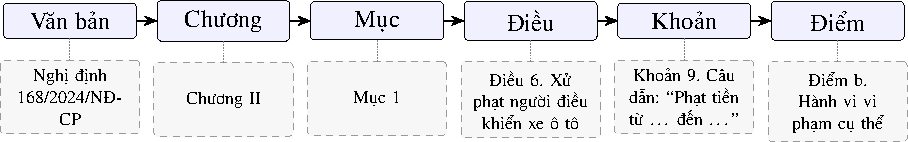
\includegraphics{graphics/fig_ch2_1.pdf}
\caption{Cấu trúc phân cấp của văn bản quy phạm pháp luật và một ví dụ trong nghị định xử phạt}
\label{fig:c2_cay_van_ban}
\end{figure}

Hai quy ước có ý nghĩa đặc biệt với việc truy hồi. Thứ nhất, trong nghị định xử phạt, mức tiền nằm ở câu dẫn của Khoản, còn hành vi nằm ở các Điểm bên dưới, nên một Điểm đứng riêng không trả lời được câu hỏi ``phạt bao nhiêu''. Thứ hai, văn bản sửa đổi chép lời văn mới trong ngoặc kép (``a) Sửa đổi, bổ sung điểm đ như sau:'' rồi tới dòng ``đ)'' trong ngoặc kép); nếu không xử lý ngoặc kép, dòng này bị hiểu nhầm thành một Điểm của chính văn bản sửa đổi. Văn bản cũng tự trích dẫn nội bộ theo khuôn mẫu ổn định như ``điểm a khoản 9 Điều này'' hay ``Điều 5 Thông tư này'', cho phép giải liên kết trích dẫn tất định trên cây đã phân tích.

\subsection{Mô hình BM25}
\label{subsec:c2_bm25}

BM25 là hàm xếp hạng thuộc khung xác suất về mức liên quan \cite{robertson2009bm25}, kết hợp trọng số nghịch đảo tần suất văn bản (IDF), theo đó từ hiếm quan trọng hơn từ phổ biến, tần suất từ có bão hoà (tham số $k_1$) và chuẩn hoá theo độ dài (tham số $b$). Với kho gồm $N$ đoạn, $n_t$ là số đoạn chứa từ $t$, IDF và điểm BM25 của đoạn $d$ đối với truy vấn $q$ là:
\begin{equation}
\label{eq:c2_idf}
\mathrm{IDF}(t) = \ln\left(1 + \frac{N - n_t + 0{,}5}{n_t + 0{,}5}\right).
\end{equation}
\begin{equation}
\label{eq:c2_bm25}
\mathrm{BM25}(q, d) = \sum_{t \in q} \mathrm{IDF}(t) \cdot \frac{\mathrm{tf}(t, d)\,(k_1 + 1)}{\mathrm{tf}(t, d) + k_1 \left(1 - b + b\,\dfrac{|d|}{\mathrm{avgdl}}\right)},
\end{equation}
trong đó $\mathrm{tf}(t, d)$ là số lần từ $t$ xuất hiện trong $d$, $|d|$ là độ dài của $d$ và $\mathrm{avgdl}$ là độ dài trung bình của các đoạn. Hệ thống dùng các giá trị thông dụng $k_1 = 1{,}2$ và $b = 0{,}75$, không chỉnh theo bộ đề. Khi $\mathrm{tf}(t,d)$ tăng, phân số trong~\eqref{eq:c2_bm25} tiến dần về $k_1 + 1$ thay vì tăng tuyến tính, nên một từ lặp nhiều lần không lấn át các từ khác; khi $|d| > \mathrm{avgdl}$, điểm giảm, nên đoạn dài không được lợi chỉ vì chứa nhiều chữ. Hàm \texttt{ts\_rank} có sẵn của PostgreSQL không có hai tính chất này: nó không có IDF, nên các từ có mặt ở hầu hết các đoạn như ``xe'' hay ``giao thông'' nặng ngang từ hiếm, và nó không chuẩn hoá độ dài.

Đề tài áp dụng BM25 cho tiếng Việt mà không tách từ: văn bản được bỏ dấu, chuyển chữ thường và tách thành âm tiết; mỗi đoạn sinh ra âm tiết đơn và cặp hai âm tiết liền nhau (``đèn tín hiệu'' sinh \texttt{den\_tin} và \texttt{tin\_hieu}, đủ để phân biệt với ``tín hiệu'' đứng riêng mà không cần từ điển). Vì cả kho và câu hỏi đều bỏ dấu trước khi tách, câu gõ không dấu vẫn khớp được với văn bản có dấu.

\subsection{Tìm kiếm theo vector và độ tương tự cosine}
\label{subsec:c2_dense}

Tìm kiếm theo vector (dense retrieval) mã hoá câu hỏi và đoạn văn thành vector trong cùng một không gian, sao cho các cặp liên quan nằm gần nhau. DPR \cite{karpukhin2020dpr} dùng hai bộ mã hoá BERT huấn luyện bằng học tương phản và vượt BM25 từ 9 đến 19 điểm phần trăm về độ chính xác top-20 trên các bộ hỏi đáp miền mở. Tuy vậy, đánh giá BEIR \cite{thakur2021beir} trên 18 bộ dữ liệu cho thấy BM25 là một mốc so sánh vững và nhiều mô hình vector tụt điểm khi chuyển sang miền mới.

Mức gần nhau giữa vector câu hỏi $\mathbf{q}$ và vector đoạn $\mathbf{d}$ được đo bằng độ tương tự cosine:
\begin{equation}
\label{eq:c2_cosine}
\cos(\mathbf{q}, \mathbf{d}) = \frac{\mathbf{q} \cdot \mathbf{d}}{\lVert \mathbf{q} \rVert \, \lVert \mathbf{d} \rVert}.
\end{equation}
Khi mọi vector đã được chuẩn hoá L2, cosine bằng tích vô hướng và khoảng cách cosine bằng $1 - \cos(\mathbf{q}, \mathbf{d})$. Để không phải so câu hỏi với mọi đoạn, cơ sở dữ liệu dùng chỉ mục HNSW, một đồ thị lân cận nhiều tầng cho phép tìm lân cận gần đúng nhanh.

Theo Matryoshka Representation Learning \cite{kusupati2022mrl}, mô hình được huấn luyện sao cho các tiền tố của vector embedding cũng là biểu diễn dùng được, nên có thể cắt bớt chiều mà mất ít chất lượng. Với vector gốc $\mathbf{v} \in \mathbb{R}^{1024}$, hệ thống giữ 512 chiều đầu và chuẩn hoá lại:
\begin{equation}
\label{eq:c2_mrl}
\tilde{\mathbf{v}} = \frac{(v_1, v_2, \ldots, v_{512})}{\lVert (v_1, v_2, \ldots, v_{512}) \rVert_2}.
\end{equation}
Cắt còn một nửa số chiều giúp giảm một nửa dung lượng lưu trữ và chi phí tính khoảng cách.

\subsection{Reciprocal Rank Fusion}
\label{subsec:c2_rrf}

Tìm kiếm lai kết hợp danh sách xếp hạng của nhánh vector và nhánh BM25; hai nhánh có thang điểm khác nhau nên không cộng điểm trực tiếp được. Reciprocal Rank Fusion \cite{cormack2009rrf} chỉ dùng thứ hạng:
\begin{equation}
\label{eq:c2_rrf}
\mathrm{RRF}(d) = \sum_{r \in R} \frac{1}{k + r(d)},
\end{equation}
trong đó $R$ là tập các danh sách xếp hạng, $r(d)$ là hạng của $d$ trong danh sách $r$ (bắt đầu từ 1), và $d$ không có trong một danh sách thì không nhận số hạng tương ứng. Bài báo gốc dùng $k = 60$, giá trị được cố định trong một khảo sát thử nghiệm ban đầu chứ không suy ra từ lý thuyết; Bruch và cộng sự \cite{bruch2023fusion} cho thấy RRF nhạy với tham số này và tổ hợp lồi của các điểm đã chuẩn hoá có thể tốt hơn. Hằng số $k$ điều khiển mức chênh lệch giữa các hạng đầu. Với $k = 60$, hạng 1 nhận $1/61 \approx 0{,}0164$ còn hạng 10 nhận $1/70 \approx 0{,}0143$, nên một kết quả đứng đầu ở một nhánh nhưng vắng ở nhánh kia có thể bị một kết quả đứng thứ mười ở cả hai nhánh vượt qua. Đề tài dùng $k = 20$: hạng 1 nhận $1/21 \approx 0{,}0476$, gấp khoảng 1,6 lần hạng 10 ($1/30 \approx 0{,}0333$), giúp giữ lại các kết quả rất tốt của từng nhánh. Giá trị này được chọn bằng cách quan sát tập dev, và khác biệt so với $k = 60$ trên tập dev chỉ là 4 câu.

\subsection{Mô hình embedding Qwen3-Embedding}
\label{subsec:c2_qwen3}

Qwen3 Embedding \cite{zhang2025qwen3} là họ mô hình embedding và xếp hạng lại dựng trên mô hình nền Qwen3, hỗ trợ chọn số chiều đầu ra theo kiểu Matryoshka và nhận chỉ dẫn cho câu hỏi. Theo báo cáo kỹ thuật, cả ba cỡ đều nhận tối đa 32K token; bản 0.6B có 1024 chiều và đạt 64,33 điểm MMTEB \cite{enevoldsen2025mmteb} (trung bình theo nhiệm vụ), bản 4B có 2560 chiều và đạt 69,45, bản 8B có 4096 chiều và đạt 70,58; trong cùng bảng so sánh, multilingual-e5-large-instruct \cite{wang2024me5} đạt 63,22 và BGE-M3 \cite{chen2024m3} đạt 59,56.

Hệ thống dùng Qwen3-Embedding-0.6B, cắt từ 1024 xuống 512 chiều theo công thức~\eqref{eq:c2_mrl}. Câu hỏi được mã hoá kèm prompt truy vấn của mô hình, một dòng chỉ dẫn đứng trước câu hỏi (\texttt{Instruct: \ldots{} Query: \ldots}); các đoạn văn bản được mã hoá không kèm prompt. Bản 0.6B được chọn vì lý do thực dụng: đa ngôn ngữ, nhận chuỗi dài và chạy được trên GPU 4 GB của máy phát triển. Bản 4B cần khoảng 8 GB trọng số ở fp16 nên chưa được đo trên kho hiện tại. Các bộ đánh giá MTEB \cite{muennighoff2023mteb} và MMTEB \cite{enevoldsen2025mmteb} đều cho thấy không có mô hình nào thắng ở mọi nhiệm vụ, nên việc đo trực tiếp trên dữ liệu của bài toán là cần thiết.

\subsection{Agent dựa trên mô hình ngôn ngữ lớn và giao thức MCP}
\label{subsec:c2_agent_mcp}

Trong Naive RAG \cite{gao2023ragsurvey}, câu hỏi được dùng trực tiếp làm truy vấn và mô hình sinh câu trả lời trong một lượt. Cách này nhanh nhưng phụ thuộc hoàn toàn vào lần tìm duy nhất: nếu câu khẩu ngữ khiến bộ tìm kiếm lệch chủ đề, mô hình không có cách nào sửa. Agent theo kiểu ReAct \cite{yao2023react} dùng một vòng lặp: suy luận về bước cần làm, gọi công cụ, đọc kết quả, rồi quyết định tìm lại, đọc rộng ra hay trả lời (Hình~\ref{fig:c2_rag_agent}).

\begin{figure}[htbp]
\centering
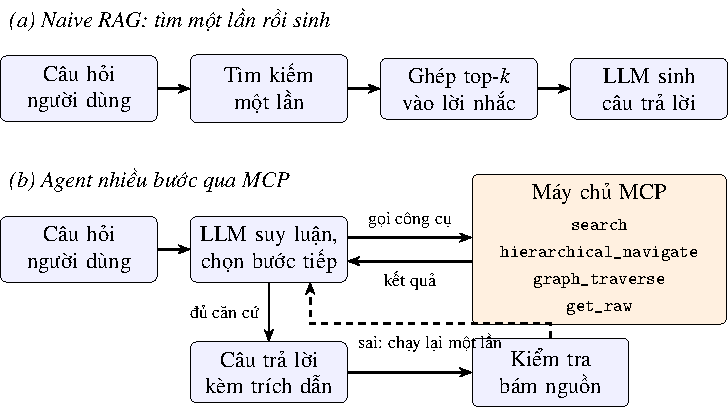
\includegraphics{graphics/fig_ch2_2.pdf}
\caption{So sánh luồng RAG tìm một lần với vòng lặp agent gọi công cụ qua MCP}
\label{fig:c2_rag_agent}
\end{figure}

Một agent cần một mô hình ngôn ngữ có khả năng gọi hàm, một tập công cụ được mô tả bằng tên, tham số và chú thích, và một vòng điều khiển giới hạn số lượt và thời gian. Khác với Toolformer \cite{schick2023toolformer} hay Self-RAG \cite{asai2024selfrag}, đề tài không huấn luyện thêm mô hình nào; hành vi của agent được điều khiển bằng lời nhắc và mô tả công cụ, nên đóng góp nằm ở thiết kế công cụ cho miền pháp luật chứ không ở cơ chế agent.

MCP \cite{anthropic2024mcp} là giao thức mở do Anthropic công bố tháng 11/2024, chuẩn hoá cách một ứng dụng dùng mô hình ngôn ngữ (client) kết nối với nguồn dữ liệu và công cụ (server): máy chủ khai báo công cụ với tên, mô tả và lược đồ tham số; client đưa mô tả cho mô hình và chuyển lời gọi do mô hình sinh ra tới máy chủ, nên cùng một máy chủ phục vụ được nhiều client mà không phải viết lại phần tích hợp. Trong đề tài, máy chủ MCP cung cấp bốn công cụ chỉ đọc \texttt{search}, \texttt{hierarchical\_navigate}, \texttt{graph\_traverse} và \texttt{get\_raw}; client là Claude Code chạy ở chế độ không tương tác, chỉ được gọi bốn công cụ này, tối đa 10 lượt và 300 giây cho mỗi câu hỏi; công cụ có khả năng ghi vào đồ thị trích dẫn nằm ngoài danh sách được phép.

\subsection{Các độ đo đánh giá}
\label{subsec:c2_do_do}

\textbf{Hit@k và MRR.} Gọi $Q$ là tập câu hỏi và $\mathrm{rank}_q$ là hạng của điều khoản đáp án đầu tiên trong kết quả cho câu hỏi $q$ (bằng $\infty$ nếu không tìm thấy, quy ước $1/\infty = 0$); một kết quả được coi là trúng khi nó là điều khoản đáp án hoặc nằm dưới điều khoản đáp án trong cây. Hit@k là tỉ lệ câu có đáp án trong $k$ kết quả đầu, còn Mean Reciprocal Rank là trung bình nghịch đảo hạng của đáp án:
\begin{equation}
\label{eq:c2_mrr}
\mathrm{Hit@}k = \frac{1}{|Q|} \sum_{q \in Q} \mathbf{1}\left[\mathrm{rank}_q \le k\right], \qquad
\mathrm{MRR} = \frac{1}{|Q|} \sum_{q \in Q} \frac{1}{\mathrm{rank}_q}.
\end{equation}
Hit@1 đo khả năng đưa đáp án lên đầu, Hit@k với $k$ lớn đo độ phủ, còn MRR thưởng cho việc đưa đáp án lên càng cao càng tốt.

\textbf{Kiểm định McNemar.} Khi so hai cấu hình A và B trên cùng một tập câu hỏi, các câu mà cả hai cùng đúng hoặc cùng sai không mang thông tin về khác biệt. Gọi $b$ là số câu A đúng mà B sai, $c$ là số câu A sai mà B đúng. Kiểm định McNemar \cite{mcnemar1947} kiểm tra giả thuyết không rằng hai loại bất đồng có cùng xác suất. Dạng chính xác dùng phân phối nhị thức với $n = b + c$:
\begin{equation}
\label{eq:c2_mcnemar}
p = \min\left(1,\; 2 \sum_{i=0}^{\min(b, c)} \binom{n}{i} \left(\frac{1}{2}\right)^{n}\right).
\end{equation}
Dạng chính xác phù hợp khi $b + c$ nhỏ, như khi hai cấu hình chỉ khác nhau ở vài câu (ví dụ đổi $k$ của RRF ở Mục~\ref{sec:ch5-tim-kiem}).

\textbf{Khoảng tin cậy Wilson.} Với tỉ lệ quan sát $\hat{p}$ trên $n$ mẫu, khoảng tin cậy Wilson ứng với giá trị tới hạn $z$ ($z = 1{,}96$ cho mức tin cậy 95\%) là:
\begin{equation}
\label{eq:c2_wilson}
\frac{\hat{p} + \dfrac{z^2}{2n} \pm z\sqrt{\dfrac{\hat{p}(1 - \hat{p})}{n} + \dfrac{z^2}{4n^2}}}{1 + \dfrac{z^2}{n}}.
\end{equation}
Khác với khoảng Wald $\hat{p} \pm z\sqrt{\hat{p}(1-\hat{p})/n}$, khoảng Wilson không vượt quá $[0, 1]$ và vẫn đáng tin khi $\hat{p}$ gần 0 hoặc 1 với mẫu nhỏ, đúng là tình huống của bộ đánh giá câu trả lời (Mục~\ref{sec:ch5-cau-tra-loi}).

\textbf{Đánh giá câu trả lời.} RAGAS \cite{es2024ragas} và ARES \cite{saadfalcon2024ares} dùng mô hình ngôn ngữ để chấm độ trung thành và độ liên quan; ALCE \cite{gao2023alce} đánh giá chất lượng trích dẫn. Đề tài chấm bằng quy tắc dựa trên đáp án tra tay (Mục~\ref{sec:ch5-cau-tra-loi}); tiêu chí ``mọi số Điều, số tiền trong câu trả lời đều có trong nguồn được trích'' là một dạng hẹp của độ trung thành và chất lượng trích dẫn, nhắm vào hai loại lỗi nguy hiểm nhất trong miền pháp luật mà \cite{magesh2025hallucination} đã chỉ ra: trích dẫn hoặc con số nghe hợp lý nhưng sai.

\section{Công nghệ sử dụng}
\label{sec:c2_cong_nghe}

Bảng~\ref{tab:c2_cong_nghe} liệt kê các công nghệ chính và vai trò của từng công nghệ trong hệ thống.

\begin{table}[htbp]
\centering
\caption{Các công nghệ sử dụng và vai trò trong hệ thống}
\label{tab:c2_cong_nghe}
\footnotesize
\renewcommand{\arraystretch}{1.05}
\begin{tabularx}{\textwidth}{@{}>{\raggedright\arraybackslash}p{4.6cm} >{\raggedright\arraybackslash}X@{}}
\toprule
\textbf{Công nghệ} & \textbf{Vai trò} \\
\midrule
Python $\geq$ 3.13, \texttt{uv} & Ngôn ngữ chính cho luồng nạp, bộ tìm kiếm, máy chủ MCP, API web và công cụ đánh giá, chạy bất đồng bộ trên \texttt{asyncio}; \texttt{uv} quản lý phụ thuộc (\texttt{uv.lock}) và chạy CLI \texttt{rag-eval} \\
PostgreSQL 16, \texttt{asyncpg} & Lưu văn bản, đoạn, chỉ mục ngược cho BM25, cạnh trích dẫn và bộ đệm vector; cài BM25 và tìm nguyên văn bằng hàm SQL; kết nối bất đồng bộ \\
\texttt{pgvector}, \texttt{ltree}, \texttt{unaccent} & Vector 512 chiều, tìm lân cận theo cosine với chỉ mục HNSW; đường dẫn phân cấp Chương--Điều--Khoản--Điểm, truy vấn theo nhánh cây; bỏ dấu \\
Docker Compose & Khởi chạy PostgreSQL kèm pgvector (container \texttt{pgvector/pgvector:pg16} trong \texttt{compose.yaml}) \\
\texttt{sentence-transformers}, \texttt{torch} & Chạy Qwen3-Embedding-0.6B để mã hoá câu hỏi và đoạn văn bản \\
\texttt{pdfplumber} & Nhánh trích xuất PDF (thử nghiệm) \\
FastAPI, \texttt{uvicorn}, Pydantic & API web cho hỏi đáp, tra cứu, danh mục văn bản và bộ đánh giá; kiểm tra dữ liệu vào ra \\
React 18, Vite, TypeScript, Tailwind CSS & Giao diện trang đơn gồm thẻ hỏi đáp, tra cứu điều luật và đánh giá tìm kiếm; song ngữ, ba chế độ màu \\
Claude Code CLI (\texttt{claude -p}) & Mô hình ngôn ngữ đóng vai trò agent, chạy không tương tác và gọi công cụ tra cứu qua MCP \\
Model Context Protocol (\texttt{mcp}) & Máy chủ MCP qua stdio, đưa bốn công cụ tra cứu chỉ đọc ra cho agent và các script đánh giá \\
\texttt{ruff}, \texttt{ty}, Playwright & Kiểm tra phong cách và kiểu tĩnh (\texttt{make check}); tự động hoá trình duyệt để kiểm thử giao diện \\
Git, GitHub & Quản lý mã nguồn, phát triển theo nhánh và pull request, lưu vết các thay đổi \\
\bottomrule
\end{tabularx}
\end{table}

Các công nghệ được chọn theo ba tiêu chí: mọi dữ liệu phục vụ tìm kiếm (văn bản, vector, chỉ mục từ khoá, đồ thị trích dẫn) nằm trong một cơ sở dữ liệu duy nhất, nên cả ba nhánh tìm kiếm cùng lọc theo ngày vi phạm và phạm vi văn bản trong một truy vấn SQL; mô hình embedding chạy cục bộ trên phần cứng phổ thông, không phụ thuộc dịch vụ ngoài khi tìm kiếm; và bộ công cụ tra cứu được tách khỏi mô hình sinh qua một giao thức chuẩn, nên có thể thay agent mà không phải sửa phần tra cứu.

\chapter{Phân tích và thiết kế hệ thống}
\label{chap:phantich}

\sloppy

Chương này trình bày yêu cầu, mô hình ca sử dụng, kiến trúc cùng các quyết định thiết kế chính, và thiết kế luồng xử lý, lớp, cơ sở dữ liệu, giao diện.

\section{Phân tích yêu cầu}
\label{sec:yeucau}

\subsection{Các tác nhân}

Hệ thống có ba tác nhân. \textbf{Người dùng} là người dân hoặc người làm công tác pháp lý cần biết một hành vi bị xử phạt thế nào; câu hỏi thường dùng ngôn ngữ đời thường, có thể không dấu hoặc viết tắt. \textbf{Người phát triển} nạp văn bản mới, chạy các bộ đánh giá và theo dõi chất lượng tìm kiếm. \textbf{Agent} là mô hình ngôn ngữ lớn chạy không tương tác, chỉ được gọi bốn công cụ tra cứu chỉ đọc qua MCP để tìm điều khoản và soạn câu trả lời.

\subsection{Yêu cầu chức năng}

Các yêu cầu chức năng của hệ thống được tổng hợp trong Bảng~\ref{tab:yc-chucnang}.

\begin{table}[H]
\centering
\caption{Yêu cầu chức năng của hệ thống}
\label{tab:yc-chucnang}
\footnotesize
\begin{tabularx}{\textwidth}{@{}l X l@{}}
\toprule
\textbf{Mã} & \textbf{Yêu cầu} & \textbf{Tác nhân} \\
\midrule
FR01 & Trả lời câu hỏi viết bằng tiếng Việt tự nhiên, kể cả không dấu hoặc viết tắt; câu trả lời ngắn gọn, mỗi khẳng định có trích dẫn trỏ tới điều khoản nguồn & Người dùng \\
FR02 & Hiển thị nguyên văn điều khoản được trích, kèm số hiệu văn bản, địa chỉ Điều--Khoản--Điểm và ngày hiệu lực & Người dùng \\
FR03 & Tra cứu điều khoản theo một tình huống và trả về nguyên văn, không qua tóm tắt & Người dùng \\
FR04 & Lọc kết quả theo ngày xảy ra vi phạm, chỉ giữ quy định còn hiệu lực vào ngày đó, và theo danh sách văn bản & Người dùng \\
FR05 & Chế độ ``Tra cứu kỹ hơn'': agent tự diễn đạt lại truy vấn, tra cứu qua nhiều bước rồi lựa chọn điều khoản & Người dùng, Agent \\
FR06 & Gắn ghi chú khi một điều khoản đã bị văn bản khác sửa đổi, bổ sung hoặc bãi bỏ và quy định sửa đổi đã có hiệu lực & Người dùng \\
FR07 & Kiểm tra câu trả lời bám nguồn: số hiệu Điều và số tiền trong câu trả lời phải xuất hiện trong các điều khoản được trích; nếu không, yêu cầu agent trả lời lại một lần & Hệ thống \\
FR08 & Chuyển ngôn ngữ giao diện Việt/Anh và chế độ màu sáng, tối hoặc tự động & Người dùng \\
FR09 & Nạp văn bản Word: chuyển thành văn bản chuẩn, phân tích cấu trúc, tạo đoạn, liên kết trích dẫn và tính vector & Người phát triển \\
FR10 & Cung cấp bốn công cụ tra cứu chỉ đọc qua máy chủ MCP & Agent \\
FR11 & Xem, chỉnh sửa và chạy bộ đánh giá tìm kiếm trên giao diện; chạy bộ đánh giá câu trả lời bằng dòng lệnh & Người phát triển \\
FR12 & Xuất và nhập toàn bộ cơ sở dữ liệu dưới dạng bản chụp (snapshot) để tái lập kết quả đo & Người phát triển \\
\bottomrule
\end{tabularx}
\end{table}

\subsection{Yêu cầu phi chức năng}

Để có thể kiểm chứng, mỗi yêu cầu phi chức năng được gắn với một chỉ tiêu định lượng. Bảng~\ref{tab:yc-phichucnang} nêu chỉ tiêu do nhóm đặt ra và kết quả đo thực tế trên kho 14 văn bản gồm 6.775 đoạn; kết quả tìm kiếm được đo trên bộ 715 câu (592 câu dev, 123 câu holdout), còn kết quả câu trả lời được đo trên bộ 81 câu, trong đó 71 câu thuộc phạm vi kho văn bản.

\begin{table}[H]
\centering
\caption{Yêu cầu phi chức năng, chỉ tiêu và kết quả đo}
\label{tab:yc-phichucnang}
\footnotesize
\begin{tabularx}{\textwidth}{@{}l X l l@{}}
\toprule
\textbf{Mã} & \textbf{Yêu cầu} & \textbf{Chỉ tiêu} & \textbf{Kết quả đo} \\
\midrule
NFR01 & Độ phủ tìm kiếm: điều khoản đáp án nằm trong kết quả của lời gọi tìm kiếm đầu tiên & $\geq 90\%$ & 93,4\% dev; 97,6\% holdout \\
NFR02 & Độ chính xác câu trả lời: đúng Điều, đủ mức tiền, đủ dữ kiện và bám nguồn & $\geq 90\%$ & 97,2\% (69/71) \\
NFR03 & Số liệu trong câu trả lời bám nguồn & $\geq 95\%$ & 98,8\% \\
NFR04 & Không từ chối nhầm câu hỏi trong phạm vi & 0\% & 0\% \\
NFR05 & Độ trễ tra cứu một lần, gồm mã hoá câu hỏi trên CPU và truy vấn cơ sở dữ liệu & p95 $\leq 1$ s & p50 501 ms; p95 690 ms \\
NFR06 & Độ trễ trả lời ở chế độ agent & trung vị $\leq 60$ s & 36 s; chậm nhất 105 s \\
NFR07 & Chi phí gọi mô hình cho mỗi câu hỏi ở chế độ agent & $\leq 0{,}20$ USD & 0,159 USD \\
NFR08 & Mô hình embedding chạy được trên GPU 4 GB & 4 GB & Qwen3-Embedding-0.6B, 512 chiều \\
NFR09 & An toàn: agent chỉ được gọi công cụ chỉ đọc & 4 công cụ & 4 công cụ, tối đa 10 lượt, 300 s \\
NFR10 & Tổng quát hoá: nạp văn bản mới không cần sửa mã nguồn & 0 dòng mã & 14 văn bản dùng chung một bộ phân tích \\
NFR11 & Tái lập: cùng một bản chụp dữ liệu cho cùng kết quả đo & tất định & Lược đồ theo phiên bản, bản chụp JSONL \\
NFR12 & Khả dụng: song ngữ, ba chế độ màu, dùng được trên điện thoại & có & có \\
\bottomrule
\end{tabularx}
\end{table}

Hai chỉ tiêu độ trễ chênh nhau một bậc độ lớn là có chủ đích: tra cứu một lần phải đủ nhanh để tương tác trực tiếp, còn chế độ agent đổi thời gian và chi phí lấy độ chính xác.

\section{Mô hình ca sử dụng}
\label{sec:usecase}

Biểu đồ ca sử dụng tổng quát được trình bày ở Hình~\ref{fig:usecase}. Ca ``Lọc theo ngày vi phạm và văn bản'' mở rộng ca tra cứu điều luật; ca ``Tra cứu kỹ hơn bằng agent'' mở rộng cả ca hỏi đáp lẫn ca tra cứu, đồng thời bao hàm ca ``Gọi công cụ tra cứu MCP'' của tác nhân Agent.

\begin{figure}[H]
\centering
\resizebox{0.82\textwidth}{!}{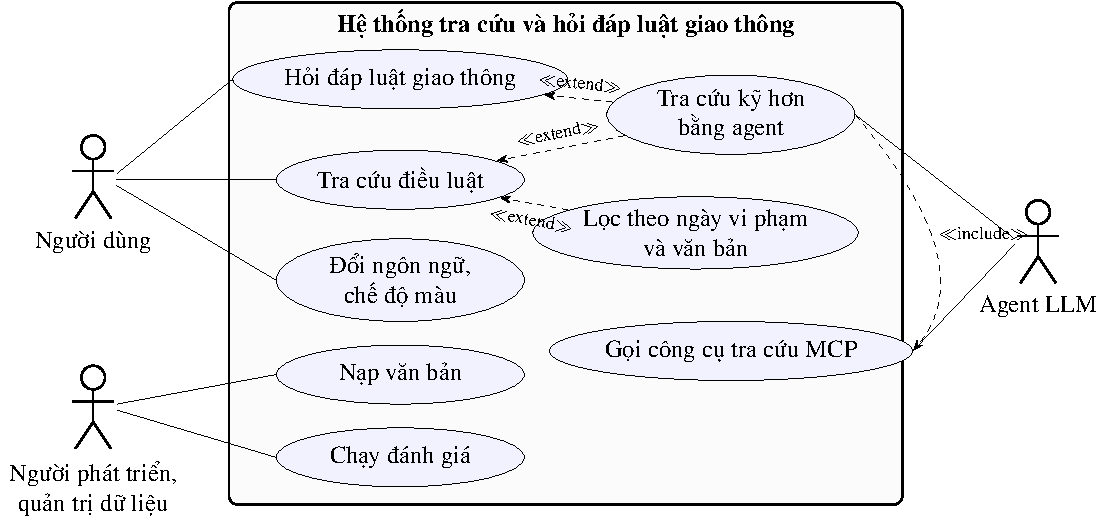
\includegraphics{graphics/fig_ch3_1.pdf}}
\caption{Biểu đồ ca sử dụng tổng quát}
\label{fig:usecase}
\end{figure}

Bảng~\ref{tab:uc-hoidap} và Bảng~\ref{tab:uc-tracuu} đặc tả hai ca sử dụng chính của người dùng; ca nạp văn bản được mô tả bằng biểu đồ hoạt động ở Mục~\ref{sec:luongxuly}.

\begin{table}[H]
\centering
\caption{Đặc tả ca sử dụng UC01: Hỏi đáp luật giao thông}
\label{tab:uc-hoidap}
\footnotesize
\begin{tabularx}{\textwidth}{@{}p{2.8cm} X@{}}
\toprule
\textbf{Tên ca sử dụng} & Hỏi đáp luật giao thông \\
\textbf{Tác nhân} & Người dùng (chính), Agent (phụ) \\
\textbf{Tiền điều kiện} & Cơ sở dữ liệu đã nạp kho văn bản; API web đang hoạt động; với chế độ agent, chương trình dòng lệnh gọi mô hình đã được cài đặt trên máy chủ \\
\textbf{Luồng chính} & 1. Người dùng nhập câu hỏi ở thẻ ``Hỏi đáp'' và giữ lựa chọn ``Tra cứu kỹ hơn''. \newline
2. Giao diện gửi yêu cầu trả lời ở chế độ agent tới API. \newline
3. Hệ thống khởi chạy agent; agent gọi các công cụ tra cứu, chọn nguồn và soạn câu trả lời có đánh số trích dẫn. \newline
4. Hệ thống đọc lại các điều khoản nguồn từ cơ sở dữ liệu, gắn ghi chú sửa đổi, đánh số lại trích dẫn và kiểm tra tính bám nguồn. \newline
5. Giao diện hiển thị câu trả lời, danh sách điều khoản nguồn và ghi chú sửa đổi. \\
\textbf{Luồng rẽ nhánh} & 3a. Người dùng bỏ chọn ``Tra cứu kỹ hơn'': hệ thống tìm kiếm một lần rồi gửi mặc định năm điều khoản cho mô hình soạn câu trả lời. \newline
4a. Kiểm tra bám nguồn không đạt: agent được chạy lại một lần kèm phản hồi; hệ thống giữ phương án có ít số liệu thiếu căn cứ hơn. \newline
4b. Ở chế độ tìm kiếm một lần, nếu không kết quả nào chứa cụm từ của câu hỏi, hệ thống thông báo không tìm thấy căn cứ mà không gọi mô hình. \\
\textbf{Ngoại lệ} & Không kết nối được máy chủ MCP, agent vượt quá 300 giây hoặc nhà cung cấp mô hình báo lỗi: API trả mã lỗi kèm lý do và không hiển thị câu trả lời. \\
\textbf{Hậu điều kiện} & Mọi điều khoản hiển thị đều được đọc từ cơ sở dữ liệu, không phải nội dung do agent tự chép lại. \\
\bottomrule
\end{tabularx}
\end{table}

\begin{table}[H]
\centering
\caption{Đặc tả ca sử dụng UC02: Tra cứu điều luật có bộ lọc}
\label{tab:uc-tracuu}
\footnotesize
\begin{tabularx}{\textwidth}{@{}p{2.8cm} X@{}}
\toprule
\textbf{Tên ca sử dụng} & Tra cứu điều luật (mở rộng: lọc theo ngày vi phạm và văn bản) \\
\textbf{Tác nhân} & Người dùng \\
\textbf{Tiền điều kiện} & Cơ sở dữ liệu đã nạp kho văn bản \\
\textbf{Luồng chính} & 1. Người dùng mô tả tình huống ở thẻ ``Tra cứu điều luật''. \newline
2. Người dùng mở bộ lọc, chọn ngày xảy ra vi phạm và một hoặc nhiều văn bản. \newline
3. Giao diện gửi yêu cầu tìm kiếm kèm ngày vi phạm và danh sách văn bản tới API. \newline
4. Hệ thống tìm kiếm lai theo vector và BM25, chỉ giữ các đoạn còn hiệu lực vào ngày vi phạm và thuộc các văn bản đã chọn, đồng thời gắn ghi chú sửa đổi. \newline
5. Giao diện hiển thị nguyên văn từng điều khoản, ngày hiệu lực và nút xem ngữ cảnh. \\
\textbf{Luồng rẽ nhánh} & 2a. Người dùng không chọn ngày: ngày vi phạm mặc định là ngày hiện tại theo giờ Việt Nam. \newline
3a. Người dùng chọn ``Tra cứu kỹ hơn'': agent lựa chọn tối đa năm điều khoản thay cho kết quả tìm kiếm thô. \newline
5a. Độ tin cậy thấp: giao diện hiển thị cảnh báo phía trên kết quả. \\
\textbf{Hậu điều kiện} & Kết quả là nguyên văn điều luật, không qua tóm tắt. \\
\bottomrule
\end{tabularx}
\end{table}

\section{Kiến trúc tổng thể}
\label{sec:kientruc}

\subsection{Kiến trúc phân tầng}

Hệ thống gồm bốn tầng (Hình~\ref{fig:kientruc}). Tầng nạp văn bản chuyển tài liệu gốc thành cây phân cấp, các đoạn và các cạnh trích dẫn. Tầng lưu trữ dùng PostgreSQL với \texttt{pgvector}, \texttt{ltree} và \texttt{unaccent}, để văn bản, vector, chỉ mục từ khoá và đồ thị trích dẫn cùng nằm trong một cơ sở dữ liệu. Tầng tra cứu và agent đóng gói các thao tác tìm kiếm, duyệt cây, duyệt đồ thị và ghi chú sửa đổi thành công cụ MCP cho agent. Tầng trên cùng gồm API web, giao diện và công cụ đánh giá.

\begin{figure}[H]
\centering
\resizebox{0.82\textwidth}{!}{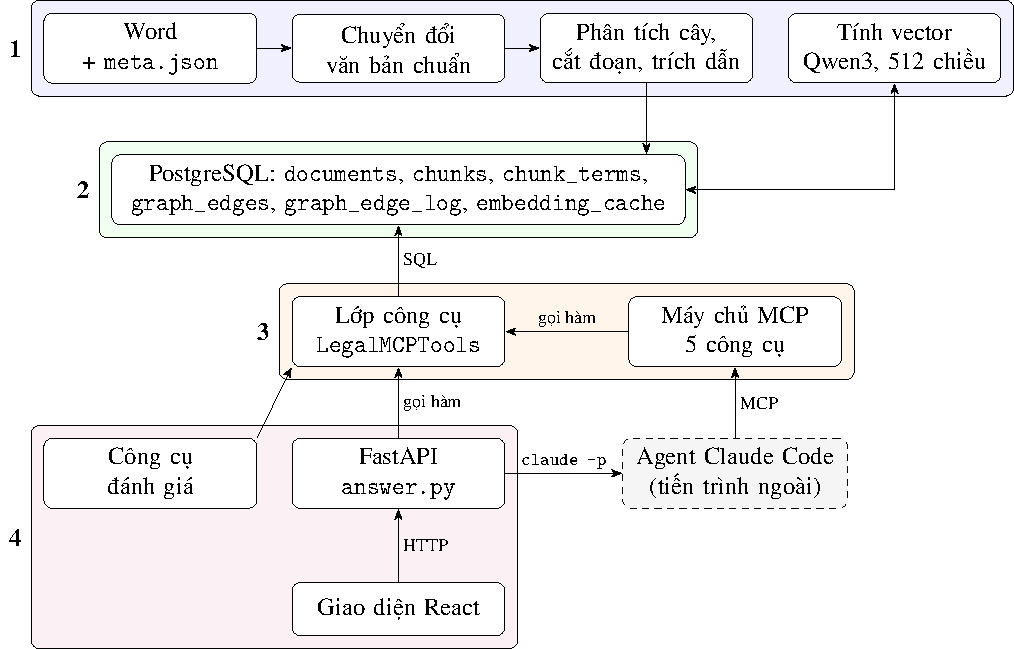
\includegraphics{graphics/fig_ch3_2.pdf}}
\caption{Kiến trúc bốn tầng: (1) nạp văn bản, (2) lưu trữ, (3) tra cứu và agent, (4) API, giao diện và đánh giá}
\label{fig:kientruc}
\end{figure}

\subsection{Các quyết định thiết kế chính}

Kiến trúc dựa trên năm quyết định thiết kế, mỗi quyết định giải quyết một đặc thù của văn bản quy phạm pháp luật tiếng Việt.

\begin{enumerate}
    \item \textbf{Phân tích cấu trúc tất định.} Văn bản được dựng thành cây Điều--Khoản--Điểm theo quy ước đánh số thay vì cắt theo độ dài cố định; hệ thống kiểm tra mỗi dòng có nội dung thuộc đúng một đoạn để lỗi phân tích không làm mất nội dung âm thầm.
    \item \textbf{Lưu nguyên văn và văn bản kèm ngữ cảnh.} Vì mức phạt nằm ở câu dẫn của Khoản còn hành vi nằm ở Điểm, mỗi đoạn được lưu thêm một phiên bản ghép tên văn bản và các câu dẫn cấp trên để tính vector và lập chỉ mục.
    \item \textbf{Tìm kiếm lai.} Nhánh vector nắm bắt ngữ nghĩa; nhánh BM25 trên âm tiết không dấu xử lý tốt câu không dấu và số hiệu; hai nhánh được hợp nhất bằng RRF, kèm tìm kiếm theo cụm từ ở tầng công cụ.
    \item \textbf{Đồ thị trích dẫn và ghi chú sửa đổi đọc từ văn bản.} Mỗi cạnh trích dẫn phải kèm cụm từ có nguyên văn trong điều khoản nguồn; ghi chú sửa đổi được suy ra từ chính các câu lệnh sửa đổi.
    \item \textbf{Kiểm tra bám nguồn.} Agent chỉ trả về câu trả lời và danh sách đường dẫn; hệ thống tự đọc nguyên văn từ cơ sở dữ liệu để hiển thị và đối chiếu số Điều, số tiền trong câu trả lời với nguồn.
\end{enumerate}

\section{Thiết kế luồng xử lý}
\label{sec:luongxuly}

\subsection{Luồng nạp văn bản}

Luồng nạp văn bản (Hình~\ref{fig:activity-ingest}) gồm ba bước độc lập. Bước chuyển đổi đọc tệp Word đúng như cách Word hiển thị rồi làm sạch thành văn bản chuẩn theo dòng; số dòng là hệ toạ độ chung của toàn hệ thống. Bước nạp phân tích cây, tạo đoạn, kiểm tra độ phủ theo dòng, liên kết trích dẫn và ghi toàn bộ kết quả trong một giao dịch. Bước tính vector chạy ngoài giao dịch để quá trình tính trên GPU không giữ khoá cơ sở dữ liệu.

\begin{figure}[H]
\centering
\resizebox{0.85\textwidth}{!}{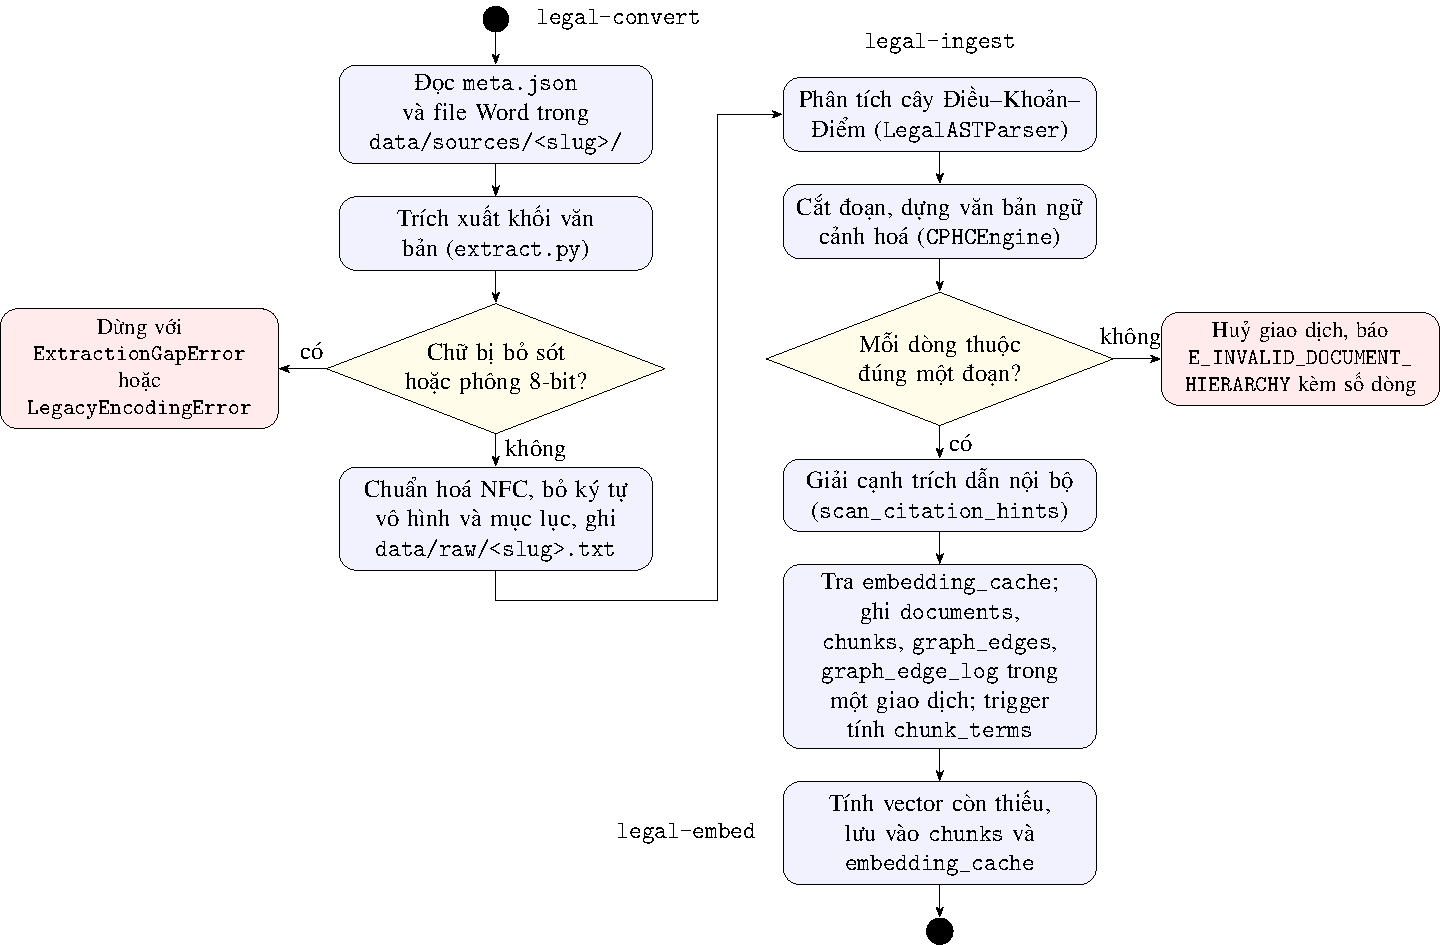
\includegraphics{graphics/fig_ch3_3.pdf}}
\caption{Biểu đồ hoạt động của luồng nạp văn bản}
\label{fig:activity-ingest}
\end{figure}

\subsection{Luồng trả lời ở chế độ agent}

Hình~\ref{fig:sequence-agent} mô tả trình tự xử lý một câu hỏi ở chế độ agent. API khởi chạy agent trong một thư mục tạm, chỉ với máy chủ MCP của hệ thống và bốn công cụ chỉ đọc. Agent tra cứu qua nhiều lượt rồi trả về câu trả lời cùng danh sách nguồn. Hệ thống đọc lại nguyên văn các nguồn từ cơ sở dữ liệu, gắn ghi chú sửa đổi, đánh số lại trích dẫn và kiểm tra bám nguồn; nếu không đạt, agent được chạy lại một lần kèm danh sách số liệu thiếu căn cứ.

\begin{figure}[H]
\centering
\resizebox{0.86\textwidth}{!}{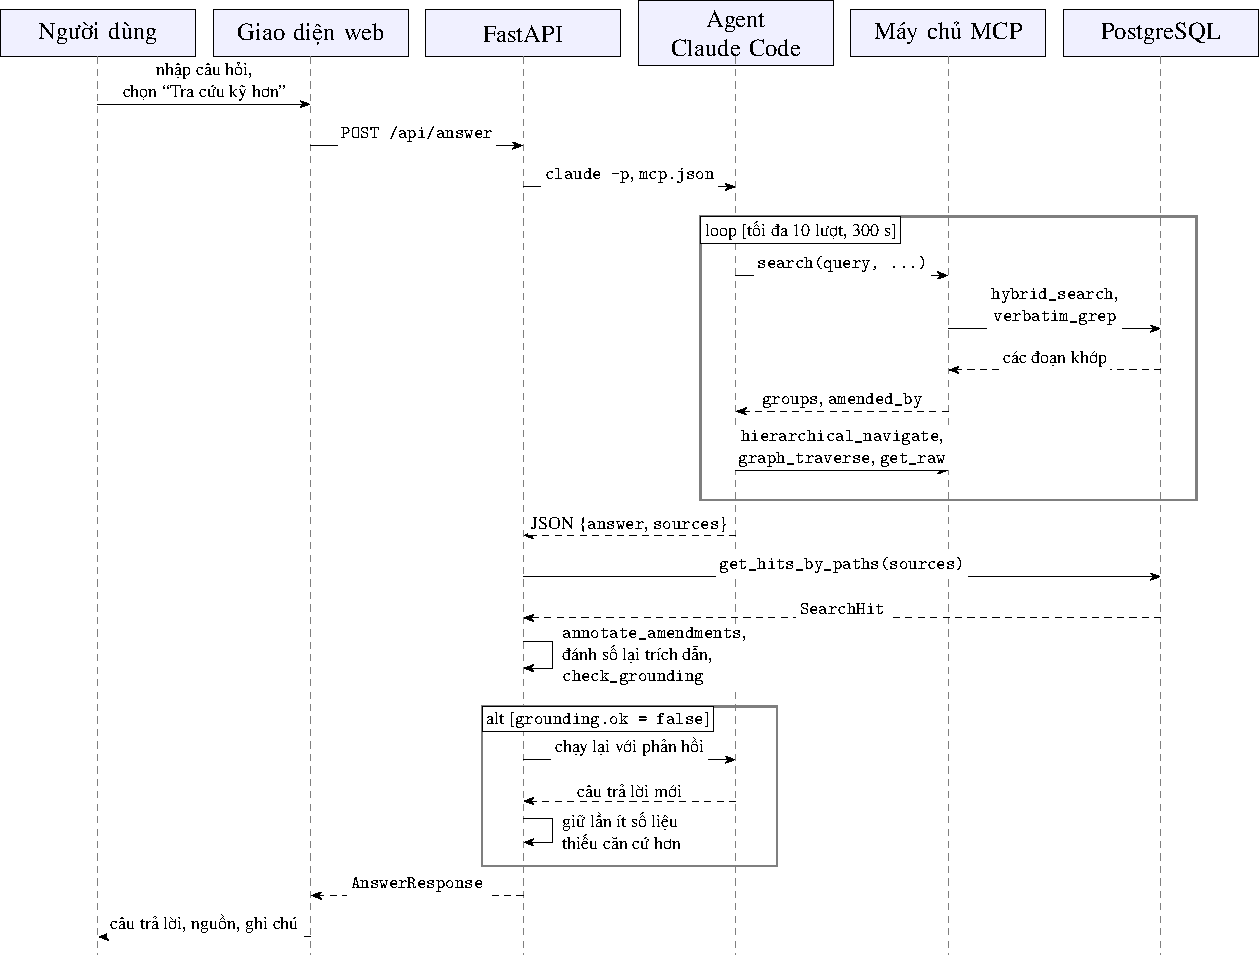
\includegraphics{graphics/fig_ch3_4.pdf}}
\caption{Biểu đồ tuần tự trả lời một câu hỏi ở chế độ agent}
\label{fig:sequence-agent}
\end{figure}

Ở chế độ tìm kiếm một lần, hệ thống bỏ qua vòng lặp gọi công cụ, tìm kiếm trực tiếp rồi gửi các điều khoản tìm được cho mô hình soạn câu trả lời trong một lượt; nếu không có kết quả nào khớp từ khoá của câu hỏi, hệ thống từ chối mà không gọi mô hình.

\section{Thiết kế lớp}
\label{sec:thietkelop}

Hình~\ref{fig:class} trình bày biểu đồ lớp của các module chính. Lớp \texttt{LegalMCPTools} là mặt tiền (facade) gom nhóm công cụ tra cứu chỉ đọc và nhóm công cụ bảo trì đồ thị, được cả máy chủ MCP lẫn API web dùng chung. Mọi kết quả tìm kiếm, duyệt cây và duyệt đồ thị đều được biểu diễn bằng cùng một kiểu \texttt{SearchHit}, có thể kèm nhiều ghi chú sửa đổi.

\begin{figure}[H]
\centering
\resizebox{0.85\textwidth}{!}{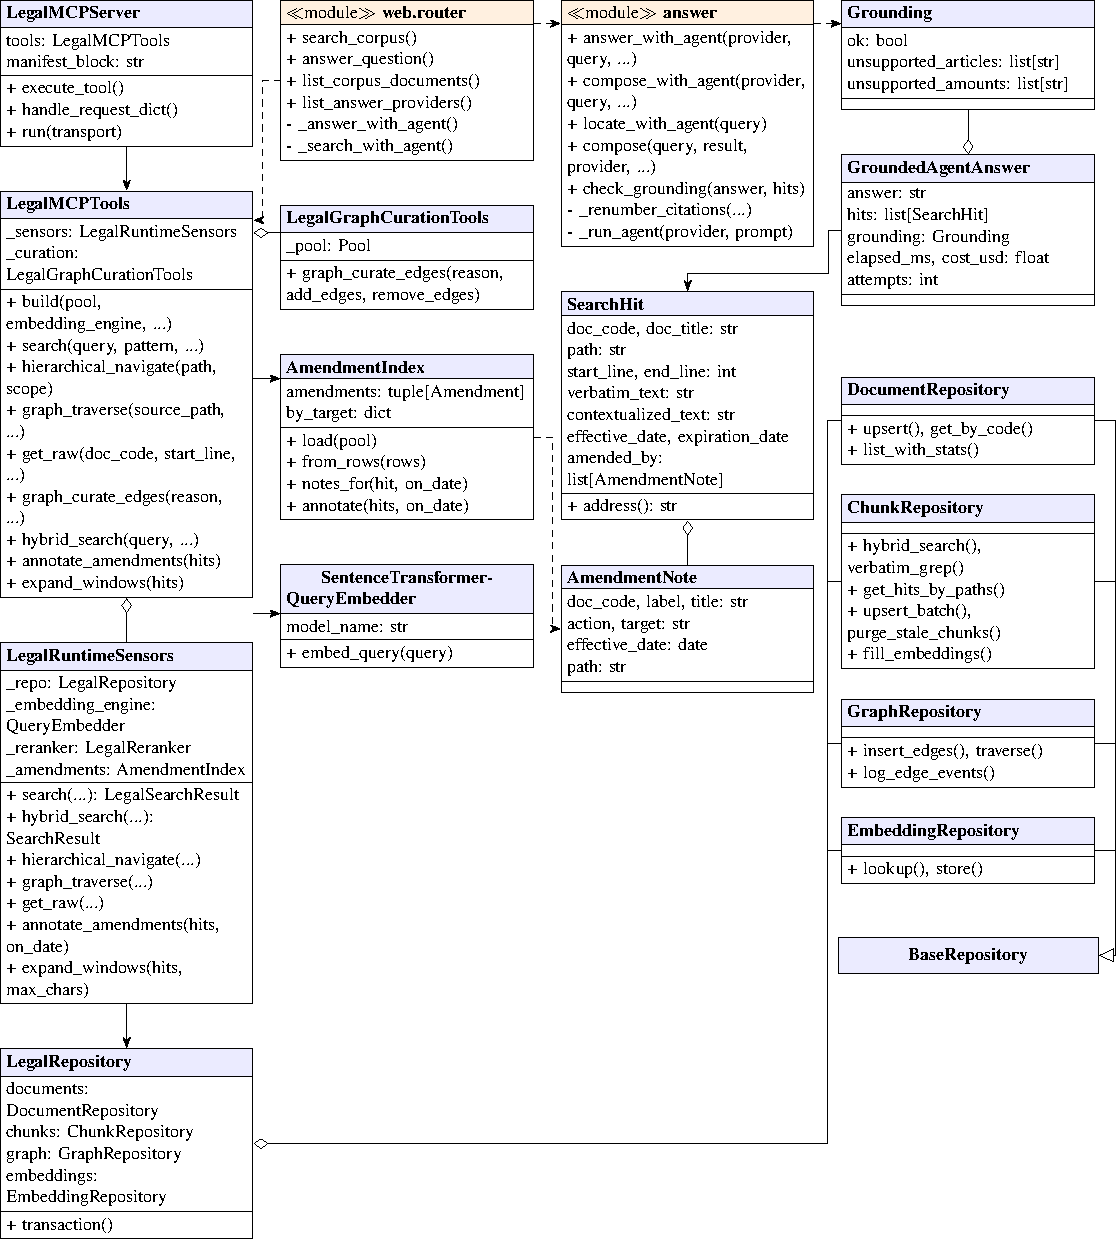
\includegraphics{graphics/fig_ch3_5.pdf}}
\caption{Biểu đồ lớp của các module chính}
\label{fig:class}
\end{figure}

\section{Thiết kế cơ sở dữ liệu}
\label{sec:csdl}

\subsection{Mô hình thực thể liên kết}

Lược đồ được xây dựng qua một chuỗi migration áp dụng theo thứ tự; Hình~\ref{fig:erd} mô tả trạng thái cuối cùng.

\begin{figure}[H]
\centering
\resizebox{\textwidth}{!}{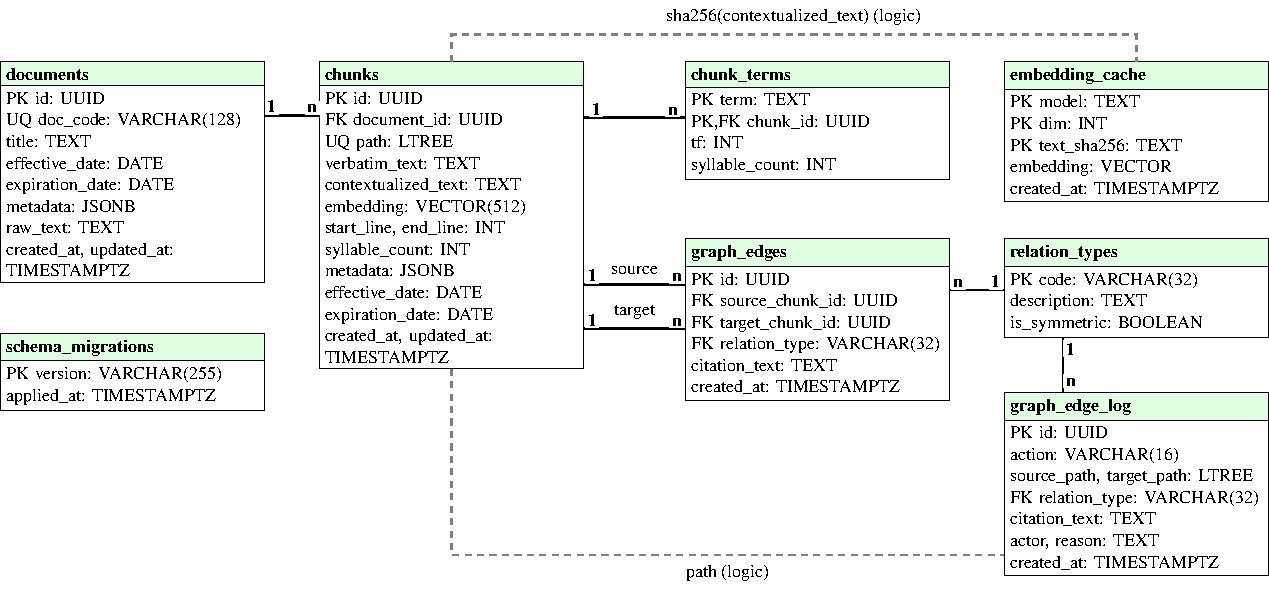
\includegraphics{graphics/fig_ch3_6.pdf}}
\caption{Mô hình thực thể liên kết của cơ sở dữ liệu (nét liền: khoá ngoại; nét đứt: liên kết logic)}
\label{fig:erd}
\end{figure}

Thiết kế có hai điểm đáng chú ý. Thứ nhất, mỗi đoạn được định danh bằng một đường dẫn phân cấp kiểu \texttt{ltree}; chẳng hạn, đường dẫn kết thúc bằng \texttt{a\_6.c\_9.p\_b} ứng với Điểm b Khoản 9 Điều 6, nhờ đó có thể lọc cả một nhánh cây cùng điều kiện hiệu lực ngay trong một câu truy vấn SQL. Thứ hai, bộ đệm vector được khoá theo mô hình, số chiều và mã băm của văn bản, nên vector được dùng lại khi nạp lại văn bản mà nội dung không đổi.

\subsection{Đặc tả các bảng}

Bảng~\ref{tab:db-chunks} đặc tả bảng chính \texttt{chunks}, còn Bảng~\ref{tab:db-khac} tóm tắt các bảng còn lại. Cột ``Ràng buộc'' sử dụng các ký hiệu PK (khoá chính), FK (khoá ngoại), UQ (duy nhất) và NN (không rỗng).

\begin{table}[H]
\centering
\caption{Bảng \texttt{chunks}: đơn vị lưu trữ và tìm kiếm}
\label{tab:db-chunks}
\footnotesize
\setlength{\tabcolsep}{3pt}
\begin{tabularx}{\textwidth}{@{}l l l X@{}}
\toprule
\textbf{Cột} & \textbf{Kiểu} & \textbf{Ràng buộc} & \textbf{Ý nghĩa} \\
\midrule
\texttt{id} & UUID & PK & Định danh đoạn \\
\texttt{document\_id} & UUID & FK, NN & Văn bản chứa đoạn (xoá theo văn bản) \\
\texttt{path} & LTREE & UQ, NN & Đường dẫn phân cấp Chương--Điều--Khoản--Điểm \\
\texttt{verbatim\_text} & TEXT & NN & Nguyên văn các dòng thuộc đoạn \\
\texttt{contextualized\_text} & TEXT & NN & Văn bản đã ghép tên văn bản, các cấp cha và câu dẫn; dùng để tính vector và lập chỉ mục BM25 \\
\texttt{embedding} & VECTOR(512) & & Vector Qwen3-Embedding-0.6B, chỉ mục HNSW theo cosine \\
\texttt{start\_line}, \texttt{end\_line} & INT & NN, CHECK & Phạm vi dòng trong văn bản chuẩn \\
\texttt{syllable\_count} & INT & NN & Số âm tiết, tức độ dài $|d|$ trong BM25; được trigger cập nhật \\
\texttt{metadata} & JSONB & NN & Loại nút, nhãn và tên Chương, Mục, Điều \\
\texttt{effective\_date} & DATE & NN & Ngày có hiệu lực \\
\texttt{expiration\_date} & DATE & CHECK & Ngày hết hiệu lực (rỗng nếu còn hiệu lực) \\
\bottomrule
\end{tabularx}
\end{table}

\begin{table}[H]
\centering
\caption{Các bảng khác của cơ sở dữ liệu}
\label{tab:db-khac}
\footnotesize
\begin{tabularx}{\textwidth}{@{}>{\raggedright\arraybackslash}p{3.4cm} >{\raggedright\arraybackslash}p{2.8cm} X@{}}
\toprule
\textbf{Bảng} & \textbf{Khoá} & \textbf{Nội dung chính} \\
\midrule
\texttt{documents} & PK \texttt{id}, UQ \texttt{doc\_code} & Số hiệu, tên văn bản, ngày hiệu lực và hết hiệu lực, siêu dữ liệu về quan hệ sửa đổi, toàn văn văn bản chuẩn \\
\texttt{chunk\_terms} & PK (\texttt{term}, \texttt{chunk\_id}) & Chỉ mục ngược cho BM25 do trigger duy trì: âm tiết hoặc cặp âm tiết không dấu, tần suất xuất hiện và độ dài đoạn \\
\texttt{graph\_edges} & PK \texttt{id}, UQ (nguồn, đích, quan hệ) & Cạnh trích dẫn giữa hai đoạn, loại quan hệ và cụm từ trích dẫn nguyên văn \\
\texttt{graph\_edge\_log} & PK \texttt{id} & Nhật ký thêm, gỡ và thu hồi cạnh, kèm tác nhân (nạp văn bản hoặc công cụ bảo trì) và lý do \\
\texttt{embedding\_cache} & PK (mô hình, số chiều, mã băm) & Vector đã tính, dùng lại khi nội dung không đổi \\
\texttt{relation\_types} & PK \texttt{code} & Danh mục loại quan hệ trích dẫn \\
\texttt{schema\_migrations} & PK \texttt{version} & Các migration đã áp dụng \\
\bottomrule
\end{tabularx}
\end{table}

Ngoài các bảng, cơ sở dữ liệu còn chứa các hàm lưu trữ đảm nhận tách âm tiết, tìm kiếm lai bằng RRF, tìm kiếm nguyên văn và duyệt đồ thị trích dẫn; cách cài đặt các hàm này được trình bày ở Chương~\ref{chap:caidat}.

\section{Thiết kế giao diện}
\label{sec:thietkegiaodien}

Giao diện là một ứng dụng trang đơn. Thanh đầu trang gồm hai thẻ dành cho người dùng, một thẻ dành cho người phát triển, cùng các nút chuyển ngôn ngữ và chế độ màu luôn hiển thị (Hình~\ref{fig:dieuhuong}).

\begin{figure}[H]
\centering
\resizebox{0.75\textwidth}{!}{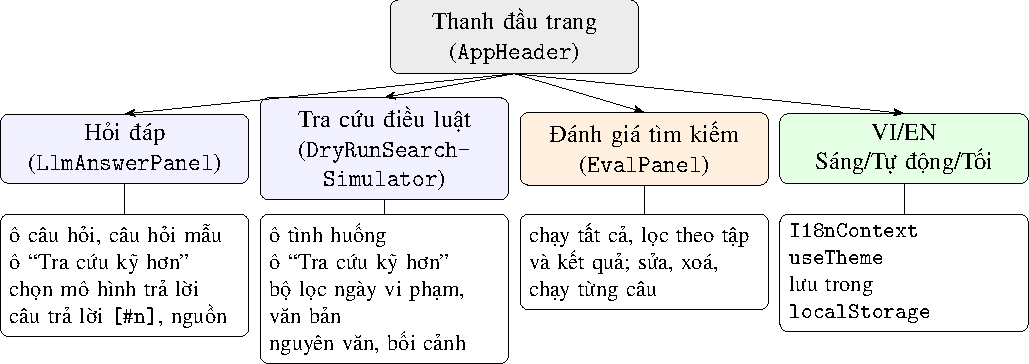
\includegraphics{graphics/fig_ch3_7.pdf}}
\caption{Cấu trúc điều hướng của giao diện}
\label{fig:dieuhuong}
\end{figure}

Giao diện được thiết kế theo bốn nguyên tắc: nguồn luôn đi cùng câu trả lời, với điều khoản nguồn và ghi chú sửa đổi hiển thị ngay bên dưới; người dùng có thể hỏi như khi nhắn tin, kể cả không dấu; kết quả có độ tương đồng thấp luôn kèm cảnh báo; và giao diện hỗ trợ hai ngôn ngữ, ba chế độ màu cùng bố cục một cột trên điện thoại.

\fussy

\chapter{Cài đặt và hiện thực hệ thống}
\label{chap:caidat}

Chương này trình bày cách hiện thực các thành phần đã thiết kế ở Chương~\ref{chap:phantich}. Nội dung đi từ môi trường và tổ chức mã nguồn, qua từng module xử lý, đến các tham số cấu hình cùng cơ sở lựa chọn, cách xử lý lỗi, bảo mật, hiệu năng, triển khai, và cuối cùng là API web cùng giao diện người dùng. Trong chương này, \emph{đoạn} (chunk) là đơn vị lưu trữ và tìm kiếm ứng với một nút của cây Điều--Khoản--Điểm, còn \emph{cạnh trích dẫn} là liên kết từ một đoạn tới đoạn mà nó viện dẫn.

\section{Môi trường và công nghệ}
\label{sec:c4_cong_nghe}

Bảng~\ref{tab:c4_cong_nghe} liệt kê các công nghệ chính, phiên bản được dùng khi đo các kết quả ở Chương~\ref{chap:kiem-thu-danh-gia} và vai trò của từng công nghệ.

\begin{table}[H]
\centering
\caption{Các công nghệ sử dụng, phiên bản và vai trò trong hệ thống}
\label{tab:c4_cong_nghe}
\footnotesize
\renewcommand{\arraystretch}{1.05}
\begin{tabularx}{\textwidth}{@{}>{\raggedright\arraybackslash}p{3.6cm} >{\raggedright\arraybackslash}p{2.6cm} >{\raggedright\arraybackslash}X@{}}
\toprule
\textbf{Công nghệ} & \textbf{Phiên bản} & \textbf{Vai trò} \\
\midrule
Python, \texttt{uv} & 3.13 & Ngôn ngữ của module nạp, bộ tìm kiếm, máy chủ MCP, API web và công cụ đánh giá; \texttt{uv} quản lý thư viện phụ thuộc \\
PostgreSQL & 16.15 & Lưu văn bản, đoạn, chỉ mục từ khoá, cạnh trích dẫn và bộ đệm vector; thực hiện BM25, RRF và tìm kiếm nguyên văn bằng hàm lưu trữ \\
\texttt{pgvector} & 0.8.6 & Kiểu vector, độ đo cosine và chỉ mục HNSW \cite{malkov2020hnsw} \\
\texttt{ltree}, \texttt{unaccent} & đi kèm PostgreSQL & Đường dẫn phân cấp và lọc theo nhánh cây; bỏ dấu tiếng Việt \\
Sentence Transformers, PyTorch & 6.0.1; 2.13.0 & Chạy Qwen3-Embedding-0.6B \cite{zhang2025qwen3} để mã hoá câu hỏi và đoạn \\
FastAPI, Pydantic, Uvicorn & 0.141; 2.13; 0.52 & API web và kiểm tra dữ liệu vào ra \\
\texttt{asyncpg} & 0.31.0 & Kết nối bất đồng bộ tới cơ sở dữ liệu \\
MCP SDK & 2.1.1 & Máy chủ Model Context Protocol \cite{anthropic2024mcp} \\
React, Vite, TypeScript, Tailwind CSS & 18.3; 6.1; 5.7; 3.4 & Giao diện trang đơn \\
Claude Code, Codex, Antigravity & bản cài đặt tại thời điểm đo & Chương trình dòng lệnh gọi mô hình ngôn ngữ lớn để trả lời (Mục~\ref{sec:cd-agent}) \\
Docker Compose & -- & Khởi chạy PostgreSQL kèm \texttt{pgvector} \\
\bottomrule
\end{tabularx}
\end{table}

Quá trình phát triển dùng thêm \texttt{ruff} và \texttt{ty} để kiểm tra phong cách mã và kiểu tĩnh, Playwright để tự động hoá trình duyệt khi kiểm thử giao diện, và Git cùng GitHub để quản lý mã nguồn theo nhánh. Phép đo độ trễ được thực hiện trên CPU Intel Xeon W-10855M (6 nhân, 32 GB RAM); việc mã hoá toàn bộ kho văn bản dùng GPU có 4 GB bộ nhớ.

Các công nghệ được lựa chọn theo ba tiêu chí. Thứ nhất, toàn bộ dữ liệu phục vụ tìm kiếm nằm trong một cơ sở dữ liệu duy nhất, nhờ đó cả ba nhánh tìm kiếm cùng lọc theo ngày vi phạm và phạm vi văn bản trong một câu truy vấn. Thứ hai, mô hình embedding chạy cục bộ trên phần cứng phổ thông, không phụ thuộc dịch vụ bên ngoài khi tìm kiếm. Thứ ba, bộ công cụ tra cứu được tách khỏi mô hình sinh qua một giao thức chuẩn, nên có thể thay chương trình trả lời mà không phải sửa phần tra cứu.

\section{Tổ chức mã nguồn}
\label{sec:cd-macnguon}

Mã nguồn được chia thành các gói tương ứng với bốn tầng của kiến trúc ở Hình~\ref{fig:kientruc}. Bảng~\ref{tab:cd-goi} trình bày ánh xạ giữa gói, tầng kiến trúc và chức năng.

\begin{table}[H]
\centering
\caption{Ánh xạ các gói mã nguồn vào kiến trúc bốn tầng}
\label{tab:cd-goi}
\footnotesize
\begin{tabularx}{\textwidth}{@{}l l X@{}}
\toprule
\textbf{Gói} & \textbf{Tầng} & \textbf{Chức năng} \\
\midrule
\texttt{ingestion} & (1) Nạp văn bản & Trích xuất tệp Word, xử lý ngoặc kép, phân tích cây, tạo đoạn, liên kết trích dẫn, tính vector \\
\texttt{db} & (2) Lưu trữ & Kết nối, 22 tệp migration lược đồ, hàm lưu trữ, xuất và nhập bản chụp dữ liệu \\
\texttt{retrieval} & (3) Tra cứu & Chỉ mục văn bản sửa đổi, bộ xếp hạng lại \\
\texttt{mcp} & (3) Tra cứu & Máy chủ MCP và các công cụ tra cứu, bảo trì đồ thị \\
\texttt{answer} & (4) Trả lời & Gọi chương trình trả lời, chế độ agent, kiểm tra bám nguồn \\
\texttt{web}, \texttt{frontend} & (4) Giao diện & API web và ứng dụng giao diện \\
\texttt{eval} & (4) Đánh giá & Chạy bộ đánh giá tìm kiếm và câu trả lời trên cùng đường xử lý của sản phẩm \\
\bottomrule
\end{tabularx}
\end{table}

Mọi thao tác vận hành, từ nạp văn bản, tính vector, chạy đánh giá đến khởi động máy chủ, đều đi qua một giao diện dòng lệnh duy nhất. Cách tổ chức này bảo đảm số liệu ở Chương~\ref{chap:kiem-thu-danh-gia} được đo trên đúng mã nguồn mà người dùng sử dụng.

\section{Module nạp văn bản}
\label{sec:cd-napvanban}

\subsection{Trích xuất văn bản nguồn}

Bước trích xuất chuyển tệp Word gốc thành văn bản chuẩn theo dòng; số dòng của văn bản chuẩn là hệ toạ độ chung cho mọi thành phần phía sau. Bước này xử lý ba đặc điểm định dạng thường gặp trong văn bản hành chính.

\begin{itemize}
    \item \textbf{Đánh số tự động.} Nhiều văn bản dùng tính năng đánh số tự động của Word cho Khoản và Điểm, nên nhãn ``1.'' hay ``a)'' không nằm trong nội dung chữ. Hệ thống khôi phục các nhãn này bằng một bộ đếm riêng cho từng cấp thụt lề.
    \item \textbf{Bảng dàn trang.} Quốc hiệu, tiêu ngữ và chữ ký thường được đặt trong bảng ẩn đường viền. Một bảng chỉ được giữ ở dạng bảng khi có khung viền bao quanh, có tối thiểu hai hàng dữ liệu và ít nhất 40\% số ô chứa nội dung; các bảng còn lại được chuyển thành văn bản thường. Ngưỡng được đặt nghiêng về phía văn bản thường vì hai loại sai có hậu quả không cân xứng: một bảng thật bị coi là văn bản vẫn giữ nguyên nội dung, còn một đoạn văn bị coi là bảng sẽ bị cắt thành các ô và mất mạch câu.
    \item \textbf{Mục lục.} Phần mục lục ở đầu một số văn bản được nhận diện và loại bỏ để không bị phân tích nhầm thành Điều.
\end{itemize}

Sau khi trích xuất, hệ thống kiểm tra rằng mọi phần tử chữ trong tệp gốc đều có mặt trong văn bản chuẩn. Một văn bản không qua được bước kiểm tra này bị từ chối nạp, thay vì được nạp với nội dung bị thiếu.

\subsection{Phân tích cấu trúc}

Trong văn bản sửa đổi, lời văn mới của điều khoản được đặt trong ngoặc kép ngay sau câu lệnh sửa đổi; chẳng hạn câu ``a) Sửa đổi, bổ sung điểm đ như sau:'' được theo sau bởi dòng ``đ)'' nằm trong ngoặc kép. Vì vậy, trước khi phân tích, hệ thống xác định mọi khoảng nằm trong ngoặc kép, kể cả trường hợp văn bản gốc thiếu dấu đóng ngoặc ở cuối dòng, và coi nội dung trong đó là văn bản thường. Bộ phân tích sau đó dựng cây theo các bước sau.

\begin{enumerate}
    \item Duyệt văn bản chuẩn theo từng dòng, giữ một ngăn xếp các nút đang mở, từ văn bản gốc xuống tới cấp sâu nhất.
    \item Với mỗi dòng nằm ngoài ngoặc kép, nhận diện ký hiệu đề mục ở đầu dòng (Phần, Chương, Mục, Điều, Khoản, Điểm) theo quy ước đánh số của từng cấp.
    \item Chỉ công nhận một ký hiệu là nút mới khi nó là số kế tiếp của nút cùng cấp đang mở, hoặc là số 1 mở đầu một cấp con. Quy tắc này ngăn việc nhận nhầm một số tiền đứng đầu dòng, chẳng hạn ``7.500 đồng'', thành Khoản 500 của Điều 7.
    \item Khi một nút mới được công nhận, đóng các nút cùng cấp hoặc sâu hơn trên ngăn xếp, rồi đặt nút mới làm con của nút đang mở gần nhất. Dòng không có ký hiệu đề mục được gán cho nút đang mở.
    \item Khi gặp phần nơi nhận hoặc chức danh người ký, ngừng nhận diện điều khoản; nếu phía sau có quy chế, quy định hoặc quy chuẩn ban hành kèm theo, mở một nút văn bản đính kèm và tiếp tục phân tích theo Điều--Khoản.
\end{enumerate}

Hai trường hợp đặc biệt cần xử lý riêng. Với các phụ lục và quy chuẩn không chia theo Điều--Khoản, như QCVN 41:2024/BGTVT, bộ phân tích nhận diện ba tầng đề mục là chữ cái, số La Mã và số thập phân, đồng thời dùng thứ tự bảng chữ cái để phân biệt chữ ``I'' đứng sau mục ``H'' với số La Mã ``I''. Ngoài ra, theo quy ước soạn thảo, các Điểm kết thúc bằng dấu chấm phẩy và Điểm cuối cùng kết thúc bằng dấu chấm; một dòng viết hoa nằm sau Điểm đã kết thúc bằng dấu chấm vì vậy được xem là đoạn kết của Khoản, trừ khi phía sau lại xuất hiện thêm một Điểm kế tiếp.

\subsection{Tạo đoạn}

Bộ tạo đoạn duyệt cây theo chiều sâu: nút lá nhận toàn bộ phạm vi dòng của nó, còn nút có con chỉ nhận phần văn bản dẫn nhập đứng trước nút con đầu tiên. Mỗi đoạn được lưu ở hai dạng: nguyên văn để hiển thị, và văn bản kèm ngữ cảnh để tính vector và lập chỉ mục từ khoá. Văn bản kèm ngữ cảnh được ghép từ tên văn bản, nhãn Chương, tên Điều, câu dẫn khung phạt của Khoản và nguyên văn của đoạn. Bảng~\ref{tab:cd-vidu-doan} minh hoạ hai dạng này với Điểm c Khoản 7 Điều 7 Nghị định 168/2024/NĐ-CP: riêng nguyên văn không cho biết hành vi thuộc loại xe nào và bị phạt bao nhiêu, trong khi văn bản kèm ngữ cảnh chứa đủ cả hai thông tin.

\begin{table}[H]
\centering
\caption{Nguyên văn và văn bản kèm ngữ cảnh của Điểm c Khoản 7 Điều 7 Nghị định 168/2024/NĐ-CP}
\label{tab:cd-vidu-doan}
\footnotesize
\begin{tabularx}{\textwidth}{@{}>{\raggedright\arraybackslash}p{2.6cm} >{\raggedright\arraybackslash}X@{}}
\toprule
\textbf{Dạng} & \textbf{Nội dung} \\
\midrule
Nguyên văn & c) Không chấp hành hiệu lệnh của đèn tín hiệu giao thông; \\
Kèm ngữ cảnh & [Nghị định quy định xử phạt vi phạm hành chính về trật tự, an toàn giao thông trong lĩnh vực giao thông đường bộ; trừ điểm, phục hồi điểm giấy phép lái xe] > [Chương II] > [Điều 7: Xử phạt, trừ điểm giấy phép lái của người điều khiển xe mô tô, xe gắn máy, các loại xe tương tự xe mô tô và các loại xe tương tự xe gắn máy vi phạm quy tắc giao thông đường bộ] > [Khoản 7: Phạt tiền từ 4.000.000 đồng đến 6.000.000 đồng đối với người điều khiển xe thực hiện một trong các hành vi vi phạm sau đây] \newline c) Không chấp hành hiệu lệnh của đèn tín hiệu giao thông; \\
\bottomrule
\end{tabularx}
\end{table}

Tiêu đề Chương chỉ được giữ ở dạng nhãn ngắn để không lặp lại ở hàng trăm đoạn, trong khi tiêu đề Phụ lục được giữ nguyên vì thường chứa tên nhóm biển báo hoặc tên bảng kỹ thuật. Văn bản kèm ngữ cảnh của mỗi đoạn được giới hạn ở 25.000 ký tự, kể cả phần ngữ cảnh; đoạn nào vượt giới hạn được chia theo ranh giới dòng thành nhiều cửa sổ, mỗi cửa sổ lặp lại tên bảng, đơn vị tính và dòng tiêu đề cột. Với kho hiện tại, chỉ 4 trong 6.775 đoạn phải chia cửa sổ, và đoạn dài nhất có 24.915 ký tự. Cuối cùng, hệ thống kiểm tra điều kiện phủ dòng: mỗi dòng có nội dung, trừ dòng tiêu đề và biểu mẫu, phải thuộc về đúng một đoạn; nếu không, quá trình nạp dừng lại và báo số dòng bị thiếu hoặc bị trùng.

\subsection{Liên kết trích dẫn}

Bộ liên kết chỉ tạo cạnh cho các cụm trích dẫn nội bộ nằm ngoài ngoặc kép và được neo bởi từ ``này'', như ``điểm a khoản 9 Điều này''. Các trích dẫn sang văn bản khác không được tạo tự động, vì việc xác định chính xác văn bản đích đòi hỏi kiểm chứng thêm (Mục~\ref{sec:cd-mcp}). Bảng~\ref{tab:cd-tridan} tóm tắt các hiện tượng ngôn ngữ mà bộ liên kết xử lý.

\begin{table}[H]
\centering
\caption{Các hiện tượng trích dẫn nội bộ và cách xử lý}
\label{tab:cd-tridan}
\footnotesize
\begin{tabularx}{\textwidth}{@{}>{\raggedright\arraybackslash}p{3.2cm} >{\raggedright\arraybackslash}p{4.2cm} >{\raggedright\arraybackslash}X@{}}
\toprule
\textbf{Hiện tượng} & \textbf{Ví dụ} & \textbf{Cách xử lý} \\
\midrule
Văn bản đính kèm & ``Điều 5 Quy chế này'' & Xác định phạm vi theo loại văn bản đứng trước từ ``này'' \\
Danh sách viết gộp & ``điểm a, điểm b khoản 6 Điều này'' & Các mục đứng trước dùng chung Khoản, Điều nêu ở cuối cụm \\
Dạng thu hẹp & ``Điều 20 (điểm c khoản 3)'' & Chỉ trỏ tới Điểm c Khoản 3 Điều 20 \\
Khoảng liên tiếp & ``từ khoản 1 đến khoản 3'' & Mở rộng theo thứ tự thực tế trên cây, kể cả khoản chèn thêm như Khoản 2a \\
Cụm có nhiều cách hiểu & ``điểm a, b khoản 1, 2'' & Bỏ qua, không tạo cạnh \\
Đích ở cấp Điều, Khoản & ``khoản 2 Điều này'' & Mở rộng xuống mọi đoạn lá bên dưới \\
\bottomrule
\end{tabularx}
\end{table}

Kết quả trên kho hiện tại là 10.570 cạnh trích dẫn. Mỗi cạnh lưu kèm cụm từ trích dẫn nguyên văn, nên luôn có thể kiểm tra lại cạnh đó bằng cách đối chiếu với văn bản nguồn.

\section{Module tìm kiếm}
\label{sec:cd-timkiem}

\subsection{Biểu diễn vector}

Các đoạn được mã hoá bằng Qwen3-Embedding-0.6B. Vector đầu ra 1.024 chiều được cắt còn 512 chiều theo phương pháp Matryoshka \cite{kusupati2022mrl} rồi chuẩn hoá L2. Khi mã hoá câu hỏi, hệ thống dùng lời nhắc truy vấn do mô hình định nghĩa, còn các đoạn được mã hoá không kèm lời nhắc; Chương~\ref{chap:kiem-thu-danh-gia} cho thấy lời nhắc này cải thiện Hit@1 có ý nghĩa thống kê. Mô hình chạy ở độ chính xác FP16 trên GPU và FP32 trên CPU; khi mã hoá cả kho, các đoạn được xử lý theo lô 32, sắp từ dài đến ngắn, và kích thước lô tự giảm một nửa khi GPU hết bộ nhớ. Vì mô hình nhận tối đa 32.768 token, giới hạn 25.000 ký tự của mỗi đoạn bảo đảm không đoạn nào bị cắt khi mã hoá. Vector đã tính được lưu trong bộ đệm theo mã băm của văn bản, nên khi nạp lại một văn bản, chỉ những đoạn có nội dung thay đổi mới phải tính lại.

\subsection{Chỉ mục từ khoá}

Trước khi lập chỉ mục, các ký hiệu số chú thích dính liền vào chữ trong văn bản hợp nhất được tách ra. Văn bản kèm ngữ cảnh của mỗi đoạn được bỏ dấu, chuyển về chữ thường và tách thành âm tiết. Chỉ mục ngược lưu cả âm tiết đơn lẫn cặp hai âm tiết liền kề cùng tần suất xuất hiện, tổng cộng 995.937 bản ghi trên kho hiện tại, và được trigger cập nhật tự động mỗi khi một đoạn thay đổi.

\subsection{Quy trình tìm kiếm lai}

Toàn bộ quy trình tìm kiếm lai được thực hiện trong một hàm lưu trữ của PostgreSQL theo các bước sau, với $n$ là số kết quả cần trả về.

\begin{enumerate}
    \item Tính số đoạn $N$ và độ dài trung bình của các đoạn, là hai đại lượng dùng trong công thức BM25.
    \item Nhánh vector: lấy $\max(6n, 120)$ đoạn có khoảng cách cosine nhỏ nhất tới vector câu hỏi, chỉ trong các đoạn còn hiệu lực vào ngày vi phạm và thuộc phạm vi văn bản, nhánh cây đã chọn.
    \item Nhánh từ khoá: tách câu truy vấn thành âm tiết và cặp âm tiết, đọc các bản ghi tương ứng trong chỉ mục ngược, tính điểm BM25 \cite{robertson2009bm25} với $k_1 = 1{,}2$ và $b = 0{,}75$, rồi lấy $\max(6n, 120)$ đoạn có điểm cao nhất với cùng các điều kiện lọc.
    \item Hợp nhất hai danh sách bằng RRF \cite{cormack2009rrf} với $k = 20$; một đoạn chỉ xuất hiện ở một nhánh vẫn nhận điểm từ nhánh đó.
    \item Trả về $n$ đoạn có điểm RRF cao nhất, kèm độ tương đồng cosine và dấu hiệu cho biết đoạn có khớp ít nhất một cặp âm tiết của câu truy vấn hay không.
\end{enumerate}

Vì các điều kiện lọc được áp dụng ngay trong từng nhánh, hai nhánh luôn chọn ứng viên trên cùng một tập đoạn hợp lệ. Ở quy mô hiện tại, bộ lập kế hoạch truy vấn của PostgreSQL chọn quét tuần tự toàn bộ 6.775 đoạn rồi sắp xếp theo khoảng cách, thay vì dùng chỉ mục HNSW. Nhánh vector vì vậy là tìm kiếm chính xác: phép đo trên 715 câu của bộ đánh giá cho thấy 120 ứng viên của nhánh vector trùng hoàn toàn với kết quả tìm kiếm vét cạn. Chỉ mục HNSW chỉ được dùng khi kho lớn hơn nhiều; khi đó cần đo lại độ phủ vì việc kết hợp chỉ mục xấp xỉ với điều kiện lọc có thể làm thiếu ứng viên.

Khi câu truy vấn được gõ hoàn toàn không dấu, nhánh vector bị tắt và chỉ nhánh từ khoá được dùng. Lý do là kho văn bản được mã hoá từ chữ có dấu, nên vector của câu không dấu thường nằm xa đáp án, trong khi chỉ mục từ khoá đã bỏ dấu vẫn khớp chính xác. Hệ thống không khôi phục dấu cho câu truy vấn vì việc khôi phục dấu tự động có thể sai nghĩa và tạo thêm một nguồn lỗi khó kiểm soát.

\subsection{Công cụ tìm kiếm kết hợp}

Công cụ tìm kiếm cung cấp cho agent kết hợp tìm kiếm lai với tìm kiếm nguyên văn. Hai bước được thực hiện lần lượt: trước hết là tìm kiếm lai theo câu truy vấn, sau đó là tìm các đoạn chứa cụm từ (hoặc biểu thức chính quy) do agent chỉ định. Các kết quả của tìm kiếm nguyên văn được xếp theo độ tương đồng cosine với câu truy vấn thay vì theo thứ tự xuất hiện trong văn bản; nhờ vậy, khi một cụm từ phổ biến như ``phục hồi điểm'' khớp hàng trăm đoạn, những đoạn gần nghĩa nhất với câu hỏi vẫn được đưa lên đầu.

Kết quả cuối được xếp thành ba nhóm theo thứ tự ưu tiên. Nhóm thứ nhất gồm các kết quả của tìm kiếm lai có chứa cụm từ chỉ định, tức là được cả hai cách tìm xác nhận. Nhóm thứ hai gồm các kết quả của tìm kiếm lai không chứa cụm từ đó. Nhóm thứ ba gồm các kết quả chỉ tìm thấy nhờ tìm kiếm nguyên văn. Các điều khoản cùng ngữ cảnh cha được gom lại để không lặp lại phần tiêu đề và câu dẫn.

\subsection{Mức độ tin cậy và bộ xếp hạng lại}

Mỗi kết quả tìm kiếm được gắn một trong ba mức độ tin cậy. Mức ``không có'' được gán khi không đoạn nào khớp ít nhất một cặp âm tiết của câu truy vấn; ở chế độ trả lời một lần, mức này khiến hệ thống từ chối trả lời mà không gọi mô hình ngôn ngữ. Trên 715 câu của bộ đánh giá, không câu nào bị gán mức này, nghĩa là điều kiện từ chối không chặn nhầm câu hỏi trong phạm vi. Mức ``thấp'' được gán khi độ tương đồng cosine cao nhất nhỏ hơn 0,86 và chỉ dùng để hiển thị cảnh báo trên giao diện; câu truy vấn không dấu luôn được xếp mức ``cao'' khi đã khớp từ khoá, vì khi đó độ tương đồng vector không còn ý nghĩa.

Ngưỡng 0,86 được đặt từ phiên bản mô hình embedding trước và chưa được hiệu chỉnh lại sau khi chuyển sang Qwen3-Embedding 512 chiều. Phép đo trên 715 câu cho thấy độ tương đồng cao nhất có trung vị 0,775, phân vị thứ 5 là 0,632, và 652 câu (91\%) bị xếp mức ``thấp'' dù đều thuộc phạm vi. Vì mức ``thấp'' không ảnh hưởng tới kết quả tìm kiếm hay câu trả lời, sai lệch này không làm thay đổi các số liệu ở Chương~\ref{chap:kiem-thu-danh-gia}, nhưng làm cảnh báo trên giao diện mất giá trị thông tin. Ngưỡng cần được hiệu chỉnh lại theo phân bố đo được, chẳng hạn đặt ở phân vị thứ 5 của các câu trong phạm vi.

Mã nguồn còn có một bộ xếp hạng lại dạng cross-encoder đa ngôn ngữ (mMiniLMv2 huấn luyện trên mMARCO), chấm lại 10 kết quả đầu với độ dài tối đa 256 token. Bộ xếp hạng lại mặc định tắt và không được bật trong bất kỳ cấu hình nào ở Chương~\ref{chap:kiem-thu-danh-gia}; tác động của nó chưa được đánh giá và được xếp vào hướng phát triển.

\section{Module ghi chú văn bản sửa đổi}
\label{sec:cd-suadoi}

Bộ suy diễn sửa đổi xây dựng một chỉ mục các điều khoản bị sửa đổi theo các bước sau.

\begin{enumerate}
    \item Với mỗi văn bản sửa đổi, che toàn bộ nội dung nằm trong ngoặc kép để lời văn mới không bị hiểu nhầm là câu lệnh.
    \item Thu thập các câu mở đầu bằng động từ sửa đổi như ``sửa đổi'', ``bổ sung'', ``bãi bỏ'', ``thay thế'' hoặc ``bỏ''.
    \item Với mỗi câu lệnh, tìm câu lệnh bao ngoài gần nhất và kế thừa từ đó văn bản đích, Điều và Khoản; câu lệnh ở cấp cao nhất lấy văn bản đích từ tên văn bản được nêu trong câu.
    \item Đọc các địa chỉ điều khoản trong câu lệnh, bổ sung các cấp còn thiếu từ phạm vi kế thừa, rồi mở rộng thành danh sách các đoạn cụ thể trên cây của văn bản đích.
    \item Chỉ những câu lệnh không bao câu lệnh nào khác mới sinh ra ghi chú; câu lệnh cấp cha chỉ truyền phạm vi xuống dưới, nhờ đó khi văn bản mới chỉ sửa một Điểm, ghi chú không bị gắn lên toàn bộ Điều.
\end{enumerate}

Ba quy tắc bổ sung giúp giải đúng các dạng câu lệnh phức tạp. Với dạng ``Sửa đổi, bổ sung một số cụm từ tại khoản 2 Điều 5 bằng cụm từ\ldots'', bộ suy diễn chỉ lấy điều khoản đích đứng sau giới từ ``tại'' và bỏ qua phần đứng sau ``bằng'', để không nhận nhầm số hiệu văn bản trong cụm từ thay thế thành văn bản bị sửa đổi. Với dạng ``Bổ sung điểm d vào sau điểm c khoản 2 Điều 10'', bộ suy diễn tách điều khoản mới khỏi mốc vị trí, rồi lấy Khoản và Điều từ mốc vị trí để xác định đầy đủ địa chỉ của điểm được bổ sung. Với dạng ``Sửa đổi tên Điều 6'', ghi chú chỉ được gắn vào tiêu đề và phần thân trực tiếp của Điều, không lan xuống các Khoản và Điểm.

Trên kho hiện tại, bộ suy diễn xác định 109 câu lệnh sửa đổi với 183 địa chỉ đích và gắn ghi chú cho 366 đoạn. Khi trả kết quả tìm kiếm, ghi chú chỉ được gắn nếu câu lệnh sửa đổi đã có hiệu lực tại ngày vi phạm được xét; mỗi ghi chú cho biết văn bản sửa đổi, câu lệnh sửa đổi và ngày áp dụng.

\section{Máy chủ MCP và bảo trì đồ thị trích dẫn}
\label{sec:cd-mcp}

Máy chủ MCP giao tiếp với client qua luồng vào ra chuẩn. Khi khởi động, máy chủ đọc danh mục văn bản cùng thời hạn hiệu lực từ cơ sở dữ liệu và đưa vào phần chỉ dẫn gửi cho agent, nhờ đó agent biết chính xác các văn bản đang có trong kho. Máy chủ cung cấp năm công cụ (Bảng~\ref{tab:mcp-tools}); mọi kết quả đều kèm số hiệu văn bản, đường dẫn phân cấp và phạm vi dòng để có thể đối chiếu với văn bản gốc.

\begin{table}[H]
\centering
\caption{Các công cụ của máy chủ MCP}
\label{tab:mcp-tools}
\footnotesize
\begin{tabularx}{\textwidth}{@{}l >{\raggedright\arraybackslash}X@{}}
\toprule
\textbf{Công cụ} & \textbf{Chức năng} \\
\midrule
\texttt{search} & Tìm kiếm lai kết hợp tìm kiếm nguyên văn (Mục~\ref{sec:cd-timkiem}); lọc được theo ngày vi phạm, danh sách văn bản và nhánh cây; kết quả kèm nhóm ưu tiên và ghi chú sửa đổi \\
\texttt{hierarchical\_navigate} & Đọc các đoạn thuộc một nhánh cây, hoặc mở rộng lên Khoản cha để lấy câu dẫn khung phạt, theo đúng thứ tự trong văn bản; tối đa 100 đoạn mỗi lần gọi \\
\texttt{graph\_traverse} & Đi theo các cạnh trích dẫn từ một điều khoản; mặc định theo chiều đi, có thể chọn chiều đến hoặc cả hai chiều, độ sâu từ 1 đến 4 \\
\texttt{get\_raw} & Đọc tối đa 100 dòng liên tiếp của văn bản chuẩn theo số dòng \\
\texttt{graph\_curate\_edges} & Công cụ bảo trì: thêm hoặc gỡ cạnh trích dẫn trong một giao dịch, có kiểm chứng nguyên văn; không được cấp cho agent trả lời \\
\bottomrule
\end{tabularx}
\end{table}

Khi đọc theo nhánh cây, các đoạn chỉ được gộp khi liền kề nhau và có cùng ngữ cảnh cha, nhờ đó đoạn kết của một Khoản không bị đẩy lên trước các Điểm. Khi duyệt đồ thị, công cụ ghi nhớ các đỉnh đã thăm để tránh vòng lặp khi hai điều khoản trích dẫn lẫn nhau. Các giới hạn 100 đoạn, 100 dòng và độ sâu 4 nhằm giữ kích thước mỗi kết quả trong khả năng đọc của agent: Điều dài nhất trong kho có 113 đoạn, nên với những Điều như vậy agent đọc theo từng Khoản; còn duyệt đồ thị quá 4 bước làm số điều khoản tăng nhanh mà ít khi còn liên quan tới câu hỏi.

Công cụ thứ năm phục vụ việc bảo trì đồ thị trích dẫn, chủ yếu để bổ sung các trích dẫn liên văn bản mà bộ liên kết lúc nạp không xử lý, chẳng hạn một điều khoản của Nghị định 168/2024/NĐ-CP dẫn tới quy tắc trong Luật Trật tự, an toàn giao thông đường bộ. Mỗi cạnh mới phải kèm cụm từ trích dẫn xuất hiện nguyên văn trong điều khoản nguồn; nếu cụm từ không có trong nguồn hoặc cạnh trỏ về chính nó, toàn bộ giao dịch bị huỷ. Mọi thay đổi được ghi vào nhật ký cùng lý do, và khi văn bản được nạp lại, các cạnh vẫn thoả điều kiện kiểm chứng được giữ nguyên.

\section{Module trả lời}
\label{sec:cd-agent}

\subsection{Các chương trình trả lời}

Hệ thống gọi mô hình ngôn ngữ lớn thông qua các chương trình dòng lệnh đã được cài đặt và đăng nhập trên máy chủ, thay vì gọi trực tiếp API của nhà cung cấp. Bảng~\ref{tab:cd-providers} liệt kê các chương trình được hỗ trợ; danh sách những chương trình có sẵn trên máy được trả về qua API để giao diện hiển thị.

\begin{table}[H]
\centering
\caption{Các chương trình trả lời được hỗ trợ}
\label{tab:cd-providers}
\footnotesize
\begin{tabularx}{\textwidth}{@{}l l l X@{}}
\toprule
\textbf{Chương trình} & \textbf{Trả lời một lần} & \textbf{Chế độ agent} & \textbf{Ghi chú} \\
\midrule
Claude Code & Có & Có & Cấu hình dùng cho mọi phép đo ở Chương~\ref{chap:kiem-thu-danh-gia} \\
Codex & Có & Không & Chỉ định mô hình mà tài khoản đăng nhập được phép dùng \\
Antigravity & Có & Có & Chế độ agent cần cấp quyền trước cho bốn công cụ chỉ đọc \\
\bottomrule
\end{tabularx}
\end{table}

\subsection{Chế độ agent}

Ở chế độ agent, hệ thống khởi chạy chương trình trả lời ở chế độ không tương tác trong một thư mục tạm rỗng, với cấu hình chỉ gồm máy chủ MCP của hệ thống và danh sách công cụ được phép chỉ gồm bốn công cụ chỉ đọc. Mỗi câu hỏi có thời hạn 300 giây; với Claude Code, số lượt hội thoại của agent còn được giới hạn ở 10, trong đó một lượt có thể gồm nhiều lần gọi công cụ. Lời nhắc yêu cầu agent chỉ dùng thông tin từ công cụ, diễn đạt lại câu hỏi bằng thuật ngữ văn bản luật trước khi tìm kiếm, mở rộng lên Khoản cha để lấy mức phạt, đi theo trích dẫn và đọc điều khoản sửa đổi khi cần, rồi kết thúc bằng câu trả lời có đánh số trích dẫn cùng danh sách đường dẫn của các điều khoản nguồn.

Kết quả ở chế độ agent phụ thuộc vào mô hình thương mại đứng sau chương trình trả lời. Các phép đo ở Chương~\ref{chap:kiem-thu-danh-gia} dùng Claude Code với mô hình mặc định của tài khoản tại thời điểm đo (tháng 10/2026); nhật ký đánh giá ghi chi phí và thời gian của từng câu nhưng không ghi tên phiên bản mô hình. Đây là một hạn chế về khả năng tái lập, vì mô hình mặc định có thể thay đổi theo thời gian.

\subsection{Chế độ trả lời một lần}

Ở chế độ trả lời một lần, hệ thống tìm kiếm trực tiếp rồi gửi các điều khoản tìm được, mặc định năm và tối đa mười, cho mô hình soạn câu trả lời trong một lượt. Mỗi điều khoản được gửi ở dạng văn bản kèm ngữ cảnh để mô hình nhận được cả mức phạt nằm ở Khoản cha. Với điều khoản dạng bảng đã chia cửa sổ, hệ thống lấy cửa sổ được tìm thấy làm trung tâm rồi mở rộng đều sang hai phía cho tới khi đạt 5.000 ký tự. Giới hạn này giữ cho năm điều khoản mặc định chiếm khoảng 25.000 ký tự, dưới mức 30.000 ký tự mà Antigravity cho phép khi lời nhắc được truyền qua tham số dòng lệnh. Lời nhắc nêu rõ các điều khoản là dữ liệu để đọc chứ không phải chỉ thị, nhằm giảm nguy cơ nội dung văn bản được mô hình hiểu thành mệnh lệnh.

\subsection{Kiểm tra bám nguồn}

Sau khi có câu trả lời, hệ thống đọc lại nguyên văn các điều khoản nguồn từ cơ sở dữ liệu, gắn ghi chú sửa đổi và đánh số lại trích dẫn theo đúng thứ tự nguồn, rồi kiểm tra bám nguồn theo hai quy tắc. Thứ nhất, mọi cụm ``Điều $N$'' trong câu trả lời phải xuất hiện trong địa chỉ hoặc nội dung của ít nhất một điều khoản nguồn. Việc đối chiếu cả nội dung là cần thiết vì một điều khoản về hiệu lực thi hành có thể liệt kê các Điều bị bãi bỏ của văn bản cũ. Thứ hai, chuỗi chữ số của mọi số tiền đi kèm từ ``đồng'' trong câu trả lời phải trùng với chuỗi chữ số của một số tiền trong nội dung các điều khoản nguồn. Ở chế độ agent, nếu kiểm tra không đạt, agent được chạy lại một lần kèm danh sách số liệu không có trong nguồn, và hệ thống giữ phương án có ít số liệu thiếu căn cứ hơn.

Phép kiểm tra này được thiết kế hẹp có chủ đích và có ba giới hạn cần lưu ý khi đọc chỉ số bám nguồn ở Chương~\ref{chap:kiem-thu-danh-gia}. Một là, nó không kiểm tra Khoản và Điểm, nên một câu trả lời trích đúng Điều nhưng sai Điểm vẫn được coi là bám nguồn. Hai là, nó so sánh chuỗi chữ số, nên cách viết ``4 triệu đồng'' không khớp với ``4.000.000 đồng'' trong văn bản và bị báo nhầm là thiếu căn cứ. Ba là, một số Điều chỉ được nhắc tới trong nội dung nguồn, chứ không phải là chính nguồn được trích, vẫn được chấp nhận. Do đó, chỉ số bám nguồn phản ánh việc câu trả lời không đưa ra số Điều hay số tiền nằm ngoài văn bản đã đọc, chứ không phản ánh tính đúng đắn của việc diễn giải.

\section{Tham số cấu hình}
\label{sec:cd-thamso}

Bảng~\ref{tab:cd-thamso} tổng hợp các tham số chính của hệ thống, giá trị đang dùng và cơ sở lựa chọn. Cơ sở được chia thành ba loại: giá trị chuẩn theo tài liệu, giá trị chọn trên tập dev, và lựa chọn kỹ thuật dựa trên ràng buộc của hệ thống.

\begin{table}[H]
\centering
\caption{Các tham số cấu hình và cơ sở lựa chọn}
\label{tab:cd-thamso}
\footnotesize
\begin{tabularx}{\textwidth}{@{}>{\raggedright\arraybackslash}p{3.3cm} >{\raggedright\arraybackslash}p{2.3cm} >{\raggedright\arraybackslash}X@{}}
\toprule
\textbf{Tham số} & \textbf{Giá trị} & \textbf{Cơ sở lựa chọn} \\
\midrule
$k_1$, $b$ của BM25 & 1,2; 0,75 & Giá trị chuẩn theo tài liệu \cite{robertson2009bm25}, không tinh chỉnh \\
$k$ của RRF & 20 & Chọn trên tập dev; so với $k = 60$, cải thiện 4 câu về độ phủ nhưng chưa có ý nghĩa thống kê ($p = 0{,}125$) và không đổi trên tập holdout (Chương~\ref{chap:kiem-thu-danh-gia}) \\
Số ứng viên mỗi nhánh & $\max(6n, 120)$ & Lựa chọn kỹ thuật: đủ lớn để một đoạn xếp hạng thấp ở một nhánh vẫn có cơ hội được nhánh kia nâng lên khi hợp nhất \\
Số chiều vector & 512 & Cắt Matryoshka từ 1.024 chiều, giảm một nửa dung lượng lưu trữ \cite{kusupati2022mrl} \\
\texttt{ef\_search} của HNSW & 200 & Lớn hơn số ứng viên 120; ở quy mô hiện tại chỉ mục không được dùng (Mục~\ref{sec:cd-timkiem}) \\
Ngưỡng ``thấp'' của độ tương đồng & 0,86 & Kế thừa từ mô hình trước; đo được là chưa hiệu chỉnh, 91\% câu trong phạm vi bị xếp ``thấp'' \\
Ngưỡng nhận bảng & 40\% ô có nội dung & Lựa chọn kỹ thuật, nghiêng về phía văn bản thường để tránh làm mất mạch câu \\
Độ dài tối đa của đoạn & 25.000 ký tự & Nằm trong giới hạn 32.768 token của mô hình; chỉ 4 trong 6.775 đoạn phải chia cửa sổ \\
Ngữ cảnh mỗi điều khoản khi trả lời một lần & 5.000 ký tự & Giữ năm điều khoản dưới giới hạn 30.000 ký tự của tham số dòng lệnh \\
Số điều khoản khi trả lời một lần & 5 (tối đa 10) & Lựa chọn kỹ thuật, cân bằng giữa độ phủ và độ dài lời nhắc \\
Giới hạn agent & 300 giây; 10 lượt & Lựa chọn kỹ thuật; trung vị đo được là 36 giây, chậm nhất 105 giây \\
Giới hạn công cụ & 100 đoạn; 100 dòng; độ sâu 4 & Lựa chọn kỹ thuật, giữ kết quả trong khả năng đọc của agent \\
\bottomrule
\end{tabularx}
\end{table}

\section{Xử lý lỗi}
\label{sec:cd-loi}

Hệ thống phân biệt rõ lỗi do người dùng, lỗi do dữ liệu và lỗi do thành phần bên ngoài, và trả về mã HTTP tương ứng kèm lý do bằng tiếng Việt.

\begin{itemize}
    \item \textbf{Lỗi đầu vào} (mã 400 và 422): câu hỏi rỗng hoặc quá 500 ký tự, đường dẫn phân cấp sai định dạng, ngày vi phạm không hợp lệ, hoặc yêu cầu chế độ agent với chương trình không hỗ trợ chế độ này.
    \item \textbf{Không tìm thấy} (mã 404): thao tác trên một câu không tồn tại trong bộ đánh giá.
    \item \textbf{Thành phần bên ngoài lỗi} (mã 502): chương trình trả lời không được cài đặt, vượt thời hạn, báo lỗi, hoặc trả về câu trả lời không đúng định dạng. Khi vượt thời hạn, hệ thống dừng tiến trình agent (trên Linux là cả nhóm tiến trình con của nó) và không hiển thị câu trả lời dở dang.
    \item \textbf{Dịch vụ chưa sẵn sàng} (mã 503): mất kết nối cơ sở dữ liệu hoặc bộ công cụ tra cứu chưa khởi tạo xong.
\end{itemize}

Ở tầng dữ liệu, mọi bước ghi khi nạp văn bản nằm trong một giao dịch, nên một văn bản bị lỗi không để lại dữ liệu dở dang. Ở tầng trả lời, mức độ tin cậy ``không có'' khiến hệ thống từ chối trả lời thay vì gửi câu hỏi cho mô hình khi không có căn cứ.

\section{Bảo mật và phạm vi triển khai}
\label{sec:cd-baomat}

Hệ thống được thiết kế để chạy cục bộ trên máy của người dùng hoặc trong mạng nội bộ, và có các biện pháp bảo vệ sau. Agent trả lời chỉ được gọi bốn công cụ chỉ đọc và chạy trong một thư mục tạm rỗng, nên không thể sửa dữ liệu hay đọc mã nguồn của hệ thống. Nội dung điều luật hiển thị cho người dùng luôn được đọc lại từ cơ sở dữ liệu, không lấy từ chữ do mô hình sinh ra. Lời nhắc nêu rõ các điều khoản là dữ liệu chứ không phải chỉ thị.

Ngược lại, hệ thống chưa đáp ứng yêu cầu của một dịch vụ công khai. API không có cơ chế xác thực, cấu hình CORS cho phép mọi nguồn gốc, và các điểm cuối sửa, xoá câu trong bộ đánh giá không được bảo vệ. Mỗi yêu cầu ở chế độ agent khởi chạy một tiến trình có thể kéo dài tới 300 giây và phát sinh chi phí gọi mô hình, nên dịch vụ dễ bị quá tải nếu bị gọi liên tục. Để triển khai cho người dùng thật, cần bổ sung xác thực, giới hạn tần suất yêu cầu, hàng đợi cho chế độ agent, giới hạn nguồn gốc trong CORS, và tách các chức năng quản trị khỏi API công khai.

\section{Hiệu năng và khả năng mở rộng}
\label{sec:cd-hieunang}

Trên kho hiện tại, độ trễ trung vị và phân vị thứ 95 của một lần tìm kiếm là 50 và 85 ms khi chỉ dùng nhánh từ khoá, 364 và 515 ms khi chỉ dùng nhánh vector, và 501 và 690 ms với hệ thống đầy đủ (Chương~\ref{chap:kiem-thu-danh-gia}). Phần lớn thời gian của nhánh vector là thời gian mã hoá câu hỏi trên CPU, không phải thời gian truy vấn cơ sở dữ liệu.

Chi phí của nhánh từ khoá tăng theo hai yếu tố. Thứ nhất, mỗi lần tìm kiếm đều tính lại số đoạn và độ dài trung bình trên toàn bộ kho, một phép tính tuyến tính theo số đoạn. Thứ hai, mỗi âm tiết của câu truy vấn kéo theo toàn bộ danh sách các đoạn chứa nó, và các âm tiết phổ biến như ``xe'' hay ``giao thông'' có danh sách rất dài. Khi kho tăng lên khoảng 100 văn bản, có thể giữ hiệu năng bằng cách lưu sẵn hai đại lượng thống kê của kho trong một bảng và cập nhật khi nạp văn bản, đồng thời bỏ qua các âm tiết có tần suất văn bản quá cao, vốn đóng góp rất ít vào điểm BM25 do trọng số IDF thấp. Với nhánh vector, khi kho đủ lớn để bộ lập kế hoạch chuyển sang dùng chỉ mục HNSW, cần đo lại độ phủ dưới điều kiện lọc như đã nêu ở Mục~\ref{sec:cd-timkiem}.

\section{Triển khai}
\label{sec:trienkhai}

Hệ thống được triển khai trên một máy theo ba bước. Bước thứ nhất khởi chạy cơ sở dữ liệu PostgreSQL kèm \texttt{pgvector} bằng Docker Compose. Bước thứ hai áp dụng lần lượt 22 tệp migration lược đồ rồi nạp bản chụp dữ liệu có sẵn trong kho mã nguồn, gồm văn bản, đoạn, vector và cạnh trích dẫn, nên không cần chạy lại bước mã hoá; toàn bộ bước này mất khoảng 60 giây. Bước thứ ba khởi động API web và giao diện người dùng. Cách nạp từ bản chụp bảo đảm mọi máy chạy trên cùng một dữ liệu và cho ra cùng kết quả tìm kiếm.

Khi bổ sung văn bản mới, người phát triển đặt tệp Word cùng tệp siêu dữ liệu (số hiệu, ngày hiệu lực, quan hệ sửa đổi) vào thư mục nguồn rồi chạy lần lượt ba bước chuyển đổi, nạp và tính vector đã mô tả ở Mục~\ref{sec:luongxuly}. Chỉ mục từ khoá được trigger cập nhật trong cùng giao dịch nạp; phép đo trên một văn bản có 1.253 đoạn cho thấy việc dựng lại chỉ mục từ khoá mất 6,6 giây. Một văn bản mới không đòi hỏi sửa mã nguồn.

\section{API web và giao diện người dùng}
\label{sec:cd-api}
\label{sec:giaodien}

API web được xây dựng bằng FastAPI và dùng chung bộ công cụ tra cứu với máy chủ MCP, nên giao diện và agent đi qua cùng một đường tìm kiếm. Các điểm cuối chính được tóm tắt trong Bảng~\ref{tab:api}.

\begin{table}[H]
\centering
\caption{Các điểm cuối chính của API web}
\label{tab:api}
\footnotesize
\begin{tabularx}{\textwidth}{@{}l l X@{}}
\toprule
\textbf{Phương thức} & \textbf{Đường dẫn} & \textbf{Chức năng} \\
\midrule
POST & \texttt{/api/search} & Tra cứu điều luật, có lọc theo ngày vi phạm và văn bản; tuỳ chọn để agent lựa chọn điều khoản \\
POST & \texttt{/api/answer} & Trả lời câu hỏi ở chế độ agent hoặc chế độ một lần, kèm điều khoản nguồn và kết quả kiểm tra bám nguồn \\
GET & \texttt{/api/answer/providers} & Danh sách chương trình trả lời có sẵn trên máy chủ \\
GET & \texttt{/api/documents} & Danh mục văn bản trong kho cùng số đoạn và ngày hiệu lực \\
GET, PUT, DELETE & \texttt{/api/eval/cases} & Xem, sửa và xoá các câu trong bộ đánh giá tìm kiếm \\
POST & \texttt{/api/eval/run} & Chạy bộ đánh giá tìm kiếm và trả về các chỉ số \\
GET & \texttt{/api/health} & Kiểm tra trạng thái kết nối cơ sở dữ liệu \\
\bottomrule
\end{tabularx}
\end{table}

Giao diện người dùng là ứng dụng trang đơn viết bằng React, gọi API qua HTTP và hiển thị kết quả theo các nguyên tắc đã nêu ở Mục~\ref{sec:thietkegiaodien}. Ở thẻ Hỏi đáp (Hình~\ref{fig:ui-traloi}), mỗi trích dẫn trong câu trả lời liên kết tới thẻ điều khoản hiển thị nguyên văn đọc từ cơ sở dữ liệu, kèm khối ghi chú sửa đổi nếu có. Ở thẻ Tra cứu (Hình~\ref{fig:ui-tracuu-ky}), người dùng có thể so sánh kết quả tìm kiếm một lần với danh sách điều khoản do agent lựa chọn ở chế độ ``Tra cứu kỹ hơn''. Thẻ Đánh giá (Hình~\ref{fig:ui-danhgia}) cho phép người phát triển xem, sửa và chạy từng câu của bộ đánh giá tìm kiếm. Giao diện hỗ trợ tiếng Việt và tiếng Anh, ba chế độ màu, và bố cục một cột trên điện thoại (Hình~\ref{fig:ui-dapung}).

\begin{figure}[H]
\centering
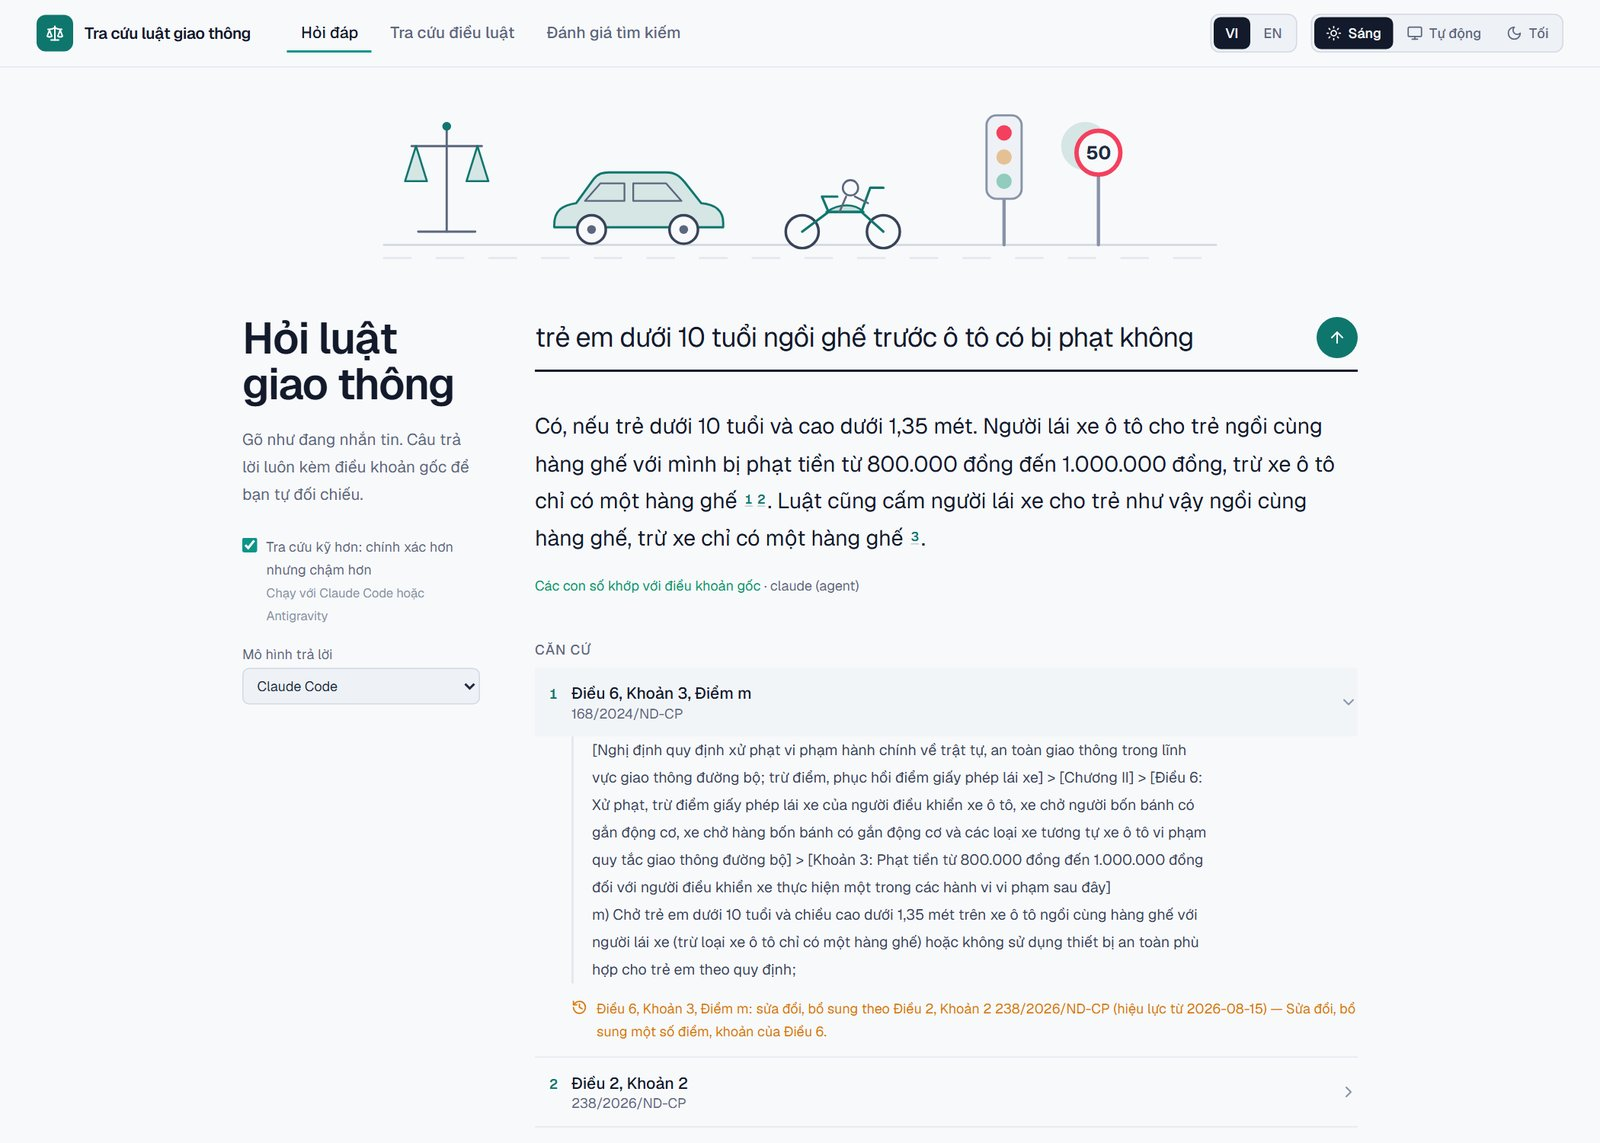
\includegraphics[width=0.88\textwidth]{graphics/ui_hoidap_traloi.jpg}
\caption[Kết quả hỏi đáp ở chế độ agent]{Kết quả hỏi đáp ở chế độ agent cho câu hỏi về trẻ em dưới 10 tuổi ngồi ghế trước ô tô: câu trả lời có trích dẫn, nguyên văn điều khoản nguồn và ghi chú sửa đổi theo Nghị định 238/2026/NĐ-CP}
\label{fig:ui-traloi}
\end{figure}

\begin{figure}[H]
\centering
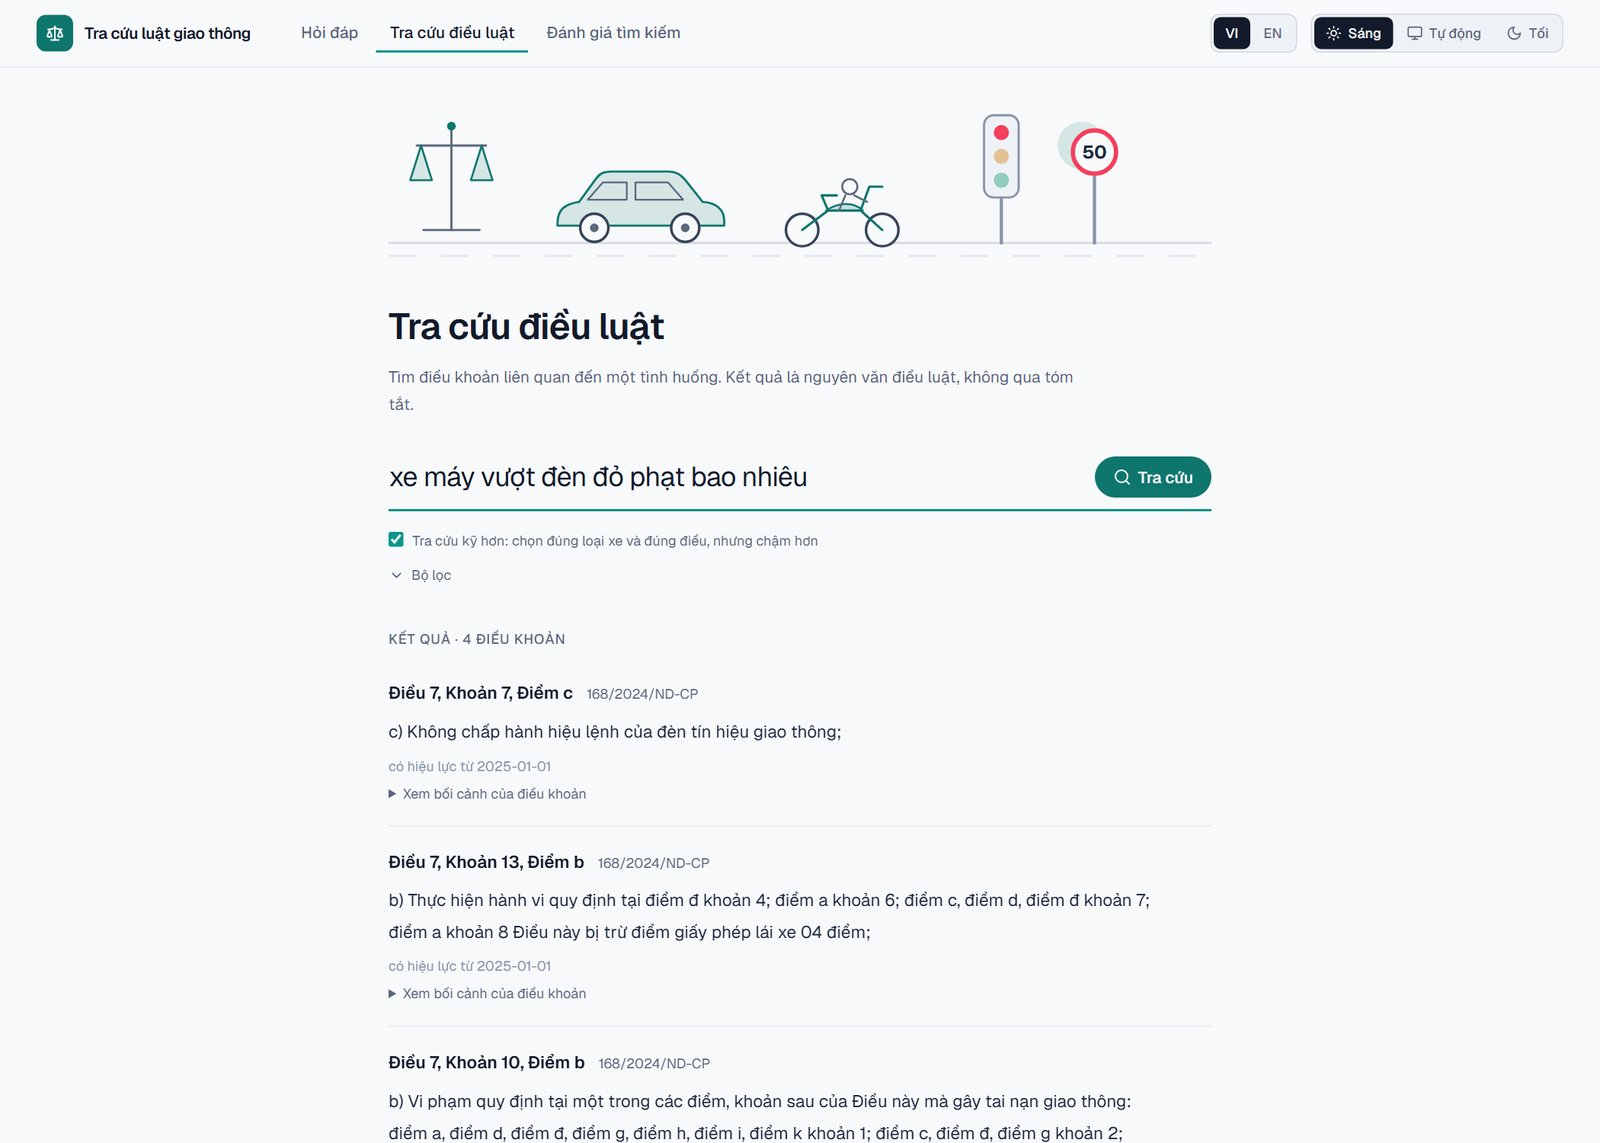
\includegraphics[width=0.78\textwidth]{graphics/ui_tracuu_ky.jpg}
\caption[Chế độ ``Tra cứu kỹ hơn'']{Chế độ ``Tra cứu kỹ hơn'' cho tình huống vượt đèn đỏ bằng xe máy: agent đưa Điểm c Khoản 7 Điều 7 Nghị định 168/2024/NĐ-CP lên đầu danh sách}
\label{fig:ui-tracuu-ky}
\end{figure}

\begin{figure}[H]
\centering
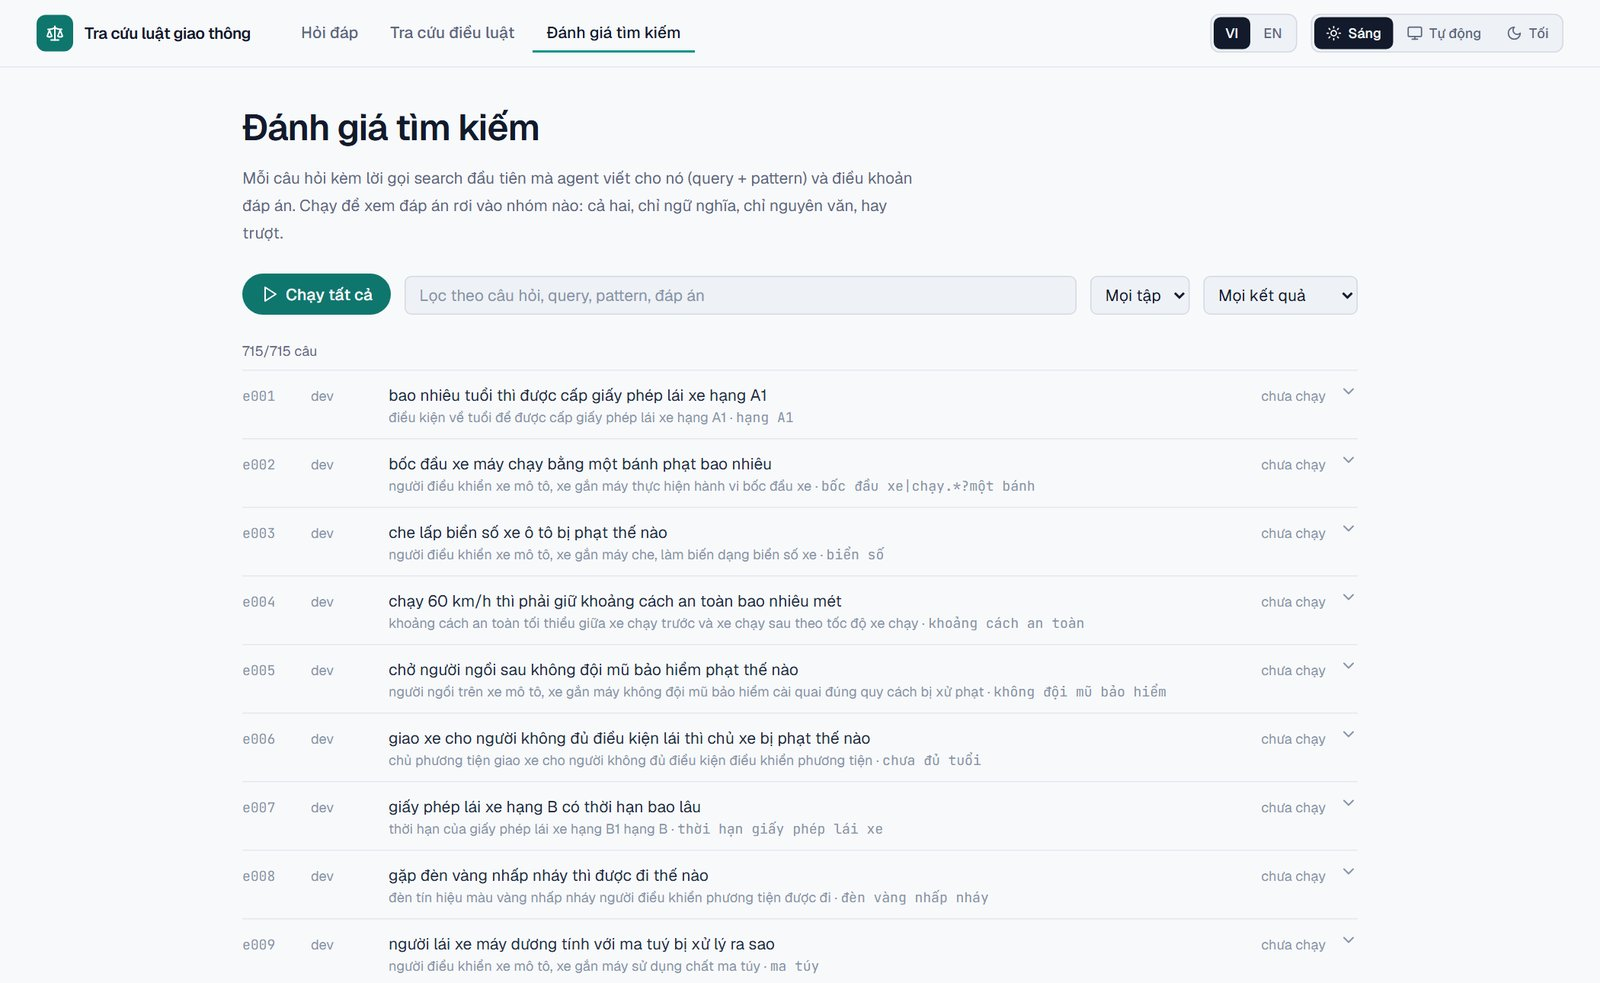
\includegraphics[width=0.78\textwidth]{graphics/ui_danhgia.jpg}
\caption{Thẻ Đánh giá: xem, sửa và chạy các câu của bộ đánh giá tìm kiếm}
\label{fig:ui-danhgia}
\end{figure}

\begin{figure}[H]
\centering
\begin{subfigure}[b]{0.62\textwidth}
  \centering
  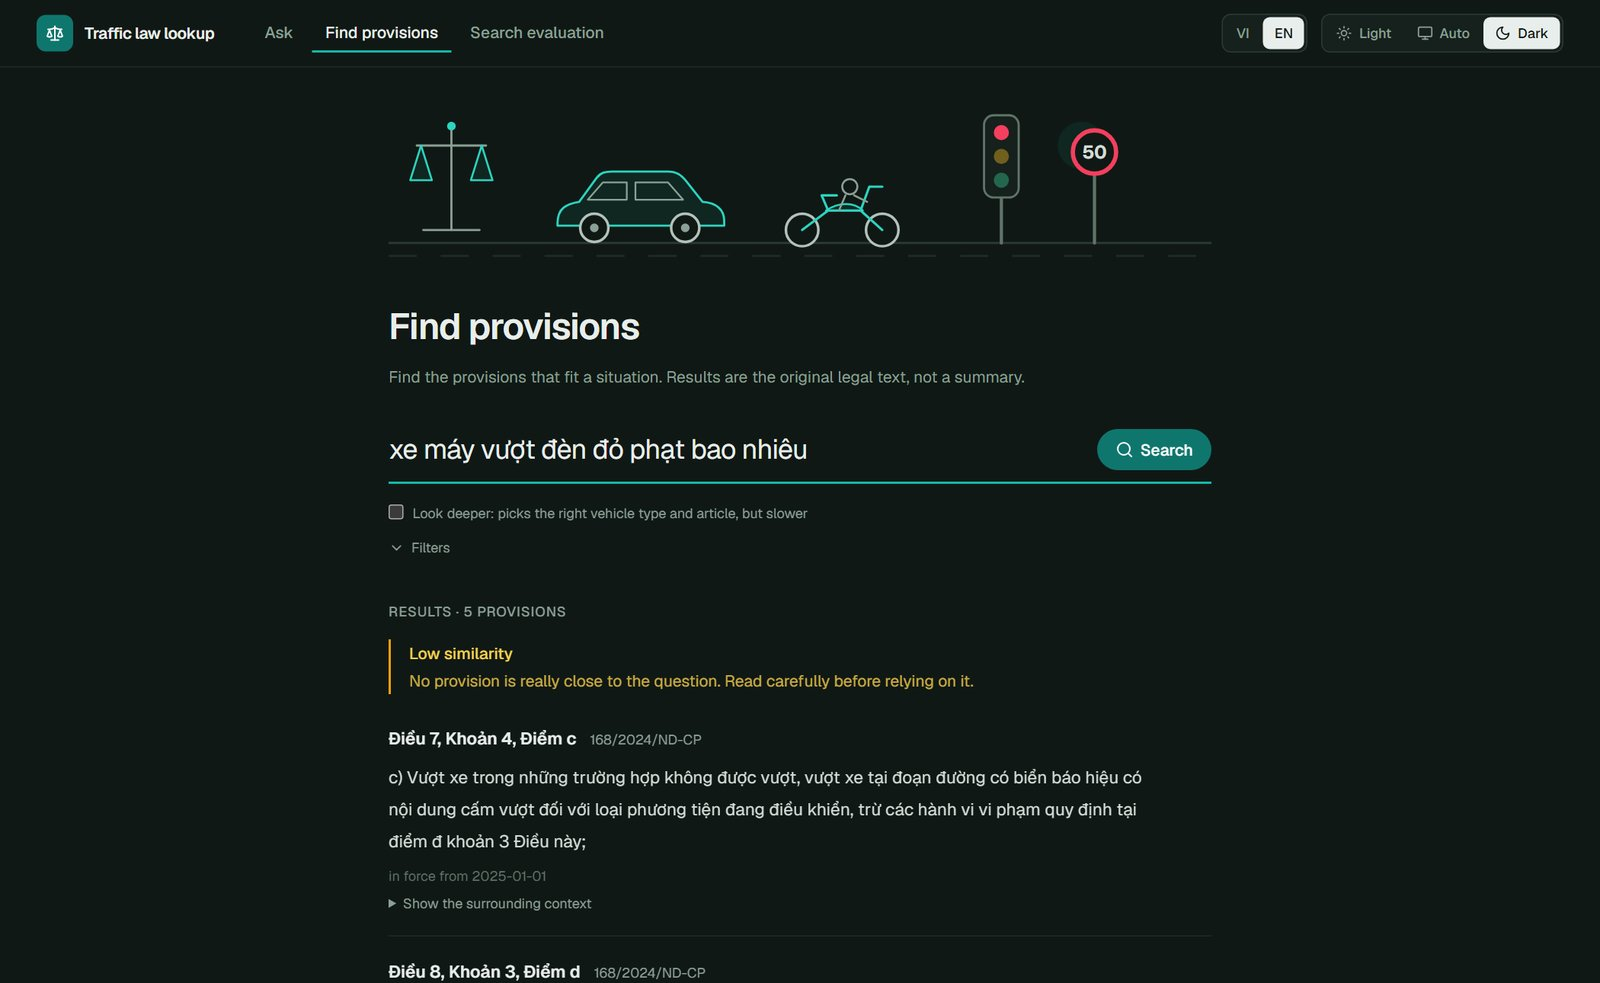
\includegraphics[width=\textwidth]{graphics/ui_tracuu_en_toi.jpg}
  \caption{Giao diện tiếng Anh, chế độ tối}
\end{subfigure}
\hfill
\begin{subfigure}[b]{0.30\textwidth}
  \centering
  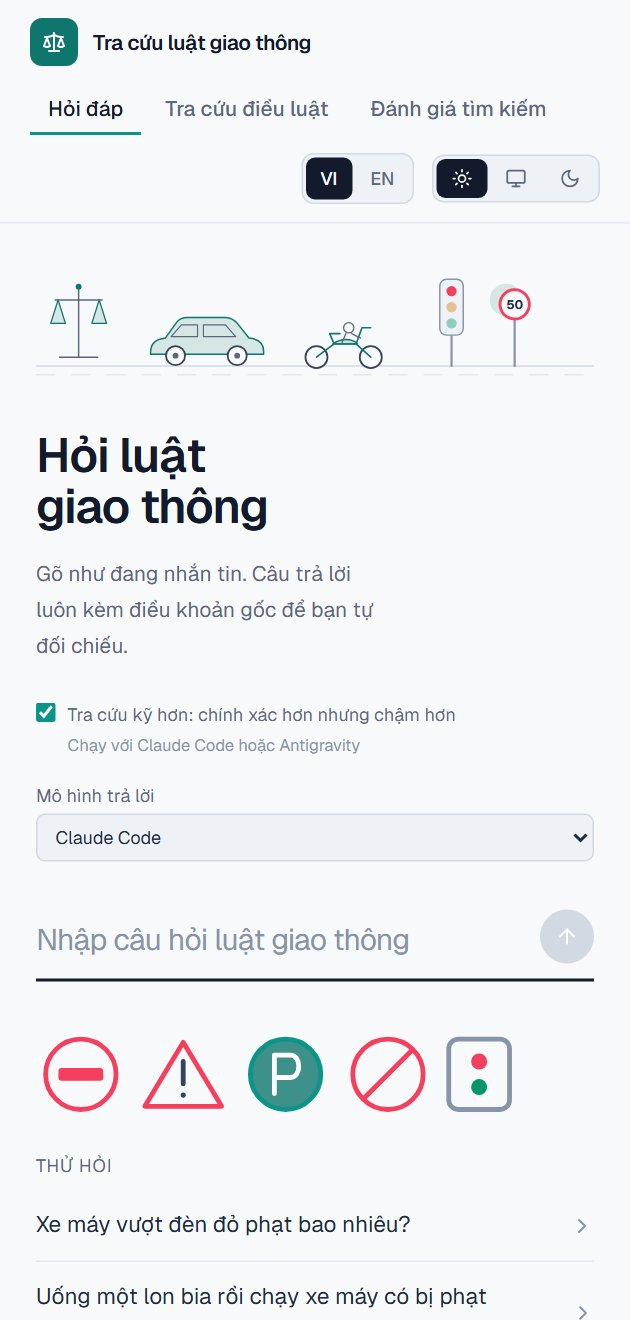
\includegraphics[width=\textwidth]{graphics/ui_mobile.jpg}
  \caption{Bố cục trên điện thoại}
\end{subfigure}
\caption{Hỗ trợ song ngữ, chế độ màu và màn hình nhỏ}
\label{fig:ui-dapung}
\end{figure}

\chapter{Kiểm thử và đánh giá}
\label{chap:kiem-thu-danh-gia}
\sloppy

\section{Đánh giá thực nghiệm tầng truy hồi}
\label{sec:ch5-ke-hoach}
\label{sec:ch5-tim-kiem}

\subsection{Thiết lập thực nghiệm và kết quả các cấu hình}

Kho dữ liệu sau khi nạp 14 văn bản quy phạm pháp luật gồm 6.775 chunk, chỉ mục ngược \texttt{chunk\_terms} chứa 995.937 bản ghi âm tiết và bigram không dấu, cùng 10.570 cạnh viện dẫn nội bộ. Bộ dữ liệu đánh giá truy hồi gồm 715 câu hỏi, chia cố định thành tập \texttt{dev} (592 câu) và tập \texttt{holdout} (123 câu). Mỗi mẫu lưu câu hỏi gốc, lời gọi \texttt{search} đầu tiên do agent sinh ra khi chỉ nhìn thấy câu hỏi và mô tả công cụ, cùng danh sách đường dẫn đáp án \texttt{expected}. Một câu được tính là \textbf{tìm thấy} nếu tập kết quả chứa ít nhất một đường dẫn thuộc tập đáp án hoặc là nút con của đáp án. Độ trễ (p50, p95) được đo tuần tự trên CPU Intel Xeon W-10855M (6 nhân, 32 GB RAM), tính cả thời gian mã hóa vector truy vấn và thực thi SQL.

Bảng~\ref{tab:ch5-ablation}, Hình~\ref{fig:ch5-tim-thay} và Hình~\ref{fig:ch5-hit1} trình bày kết quả thực nghiệm ablation trên 11 cấu hình. Các cấu hình \textbf{1--4b} không có nhánh nguyên văn \texttt{verbatim\_grep} và trả về tối đa 10 điều khoản (cột ``Tìm thấy'' tương đương $\text{Hit@10}$). Các cấu hình \textbf{5--6d} trả về tối đa 10 kết quả từ nhánh hợp nhất cộng tối đa 10 kết quả bổ sung từ nhánh nguyên văn (ở thứ hạng 11--20); do đó cột ``Tìm thấy'' chỉ so sánh trực tiếp trong từng cụm (1--4b hoặc 5--6d), còn $\text{Hit@1}$ và $\text{Hit@5}$ hoàn toàn tương đương trên mọi dòng. Nếu cắt ở top 10, tỷ lệ tìm thấy của cấu hình 5 trùng với cấu hình 4 (91,0\% trên \texttt{dev}, 95,1\% trên \texttt{holdout}). Xét theo phân bố nhóm, cấu hình 5 tìm thấy 432 câu ở \texttt{both}, 107 ở \texttt{semantic\_only}, 14 ở \texttt{verbatim\_only} và trượt 39 câu trên \texttt{dev}; trên \texttt{holdout} lần lượt là 99, 18, 3 và 3 câu.

\begin{table}[htbp]
\centering
\caption{So sánh kết quả thực nghiệm của 11 cấu hình truy hồi trên tập \texttt{dev} (592 câu) và \texttt{holdout} (123 câu)}
\label{tab:ch5-ablation}
\footnotesize
\setlength{\tabcolsep}{3pt}
\begin{tabularx}{\textwidth}{@{}l >{\raggedright\arraybackslash}X r r c c r@{}}
\toprule
\multirow{2}{*}{\textbf{\#}} & \multirow{2}{*}{\textbf{Cấu hình truy hồi}} & \multicolumn{2}{c}{\textbf{Tìm thấy (\%)}} & \textbf{Dev} & \textbf{Holdout} & \textbf{p50 / p95} \\
\cmidrule(lr){3-4}
 & & \textbf{Dev} & \textbf{Holdout} & \textbf{H@1 / H@5 / MRR} & \textbf{H@1 / H@5 / MRR} & \textbf{(ms)} \\
\midrule
1 & Chỉ vector (có \texttt{query prompt}) & 83,8 & 86,2 & 50,0 / 78,4 / 0,617 & 56,9 / 83,7 / 0,673 & 364 / 515 \\
1b & Chỉ vector (không có \texttt{query prompt}) & 81,8 & 87,0 & 47,6 / 74,8 / 0,586 & 52,8 / 79,7 / 0,633 & 278 / 399 \\
2 & Chỉ từ khóa BM25 (\texttt{chunk\_terms}) & 88,7 & 92,7 & 57,8 / 80,9 / 0,681 & 61,8 / 88,6 / 0,734 & 50 / 85 \\
3 & Chỉ từ khóa \texttt{ts\_rank} (PostgreSQL) & 67,2 & 69,9 & 13,7 / 45,8 / 0,275 & 16,3 / 50,4 / 0,286 & 38 / 78 \\
4 & Kết hợp Vector + BM25 ($\text{RRF } k=20$), không có nhánh nguyên văn & 91,0 & 95,1 & 59,3 / 82,6 / 0,695 & 63,4 / 88,6 / 0,742 & 406 / 573 \\
4b & Kết hợp Vector (không prompt) + \texttt{ts\_rank} ($\text{RRF } k=60$) & 87,2 & 91,1 & 54,7 / 80,2 / 0,655 & 60,2 / 86,2 / 0,720 & 312 / 460 \\
\midrule
\textbf{5} & \textbf{Hệ thống đầy đủ (Vector có prompt + BM25, $\text{RRF } k=20$ + nguyên văn xếp theo vector)} & \textbf{93,4} & \textbf{97,6} & 58,6 / 83,8 / 0,692 & 64,2 / 88,6 / 0,751 & 501 / 690 \\
6a & Cấu hình 5, bỏ \texttt{query prompt} & 92,7 & 96,7 & 56,2 / 84,5 / 0,679 & 64,2 / 89,4 / 0,751 & 414 / 561 \\
6b & Cấu hình 5, thay bằng $\text{RRF } k=60$ & 92,7 & 97,6 & 58,4 / 83,3 / 0,690 & 64,2 / 87,8 / 0,750 & 500 / 678 \\
6c & Cấu hình 5, nhánh nguyên văn xếp theo thứ tự văn bản & 92,7 & 97,6 & 58,6 / 83,8 / 0,692 & 64,2 / 88,6 / 0,751 & 501 / 689 \\
6d & Cấu hình cơ sở (\texttt{ts\_rank}, không prompt, $\text{RRF } k=60$, nguyên văn theo thứ tự văn bản) & 90,9 & 94,3 & 56,1 / 82,4 / 0,670 & 61,0 / 85,4 / 0,720 & 404 / 562 \\
\bottomrule
\end{tabularx}
\end{table}

\begin{figure}[htbp]
\centering
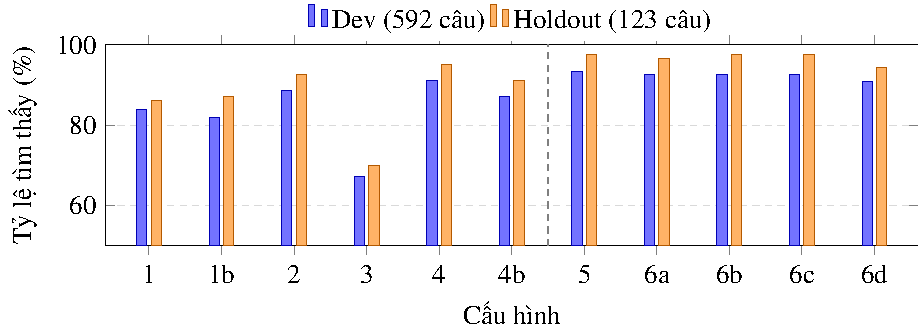
\includegraphics{graphics/fig_ch5_1.pdf}
\caption{Tỷ lệ tìm thấy đáp án theo cấu hình (dòng 1--4b: $\text{Hit@10}$; dòng 5--6d: tập kết quả đầy đủ của công cụ \texttt{search})}
\label{fig:ch5-tim-thay}
\end{figure}

\begin{figure}[htbp]
\centering
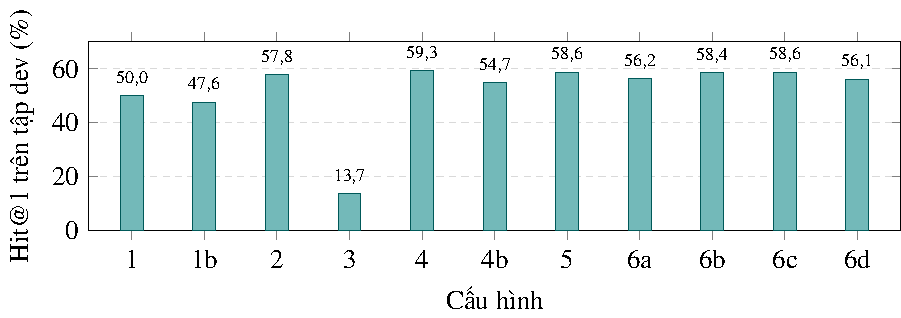
\includegraphics{graphics/fig_ch5_2.pdf}
\caption{Tỷ lệ đáp án đứng ở vị trí đầu tiên ($\text{Hit@1}$) trên tập \texttt{dev} theo từng cấu hình}
\label{fig:ch5-hit1}
\end{figure}

\subsection{Đối sánh thực nghiệm các mô hình embedding}

Bảng~\ref{tab:ch5-embedding-sweep} đối sánh mô hình \texttt{Qwen/Qwen3-Embedding-0.6B} cắt còn 512 chiều theo Matryoshka với hai mô hình cùng phân khúc 0,6 tỷ tham số giữ nguyên 1.024 chiều (\texttt{microsoft/harrier-oss-v1-0.6b} và bản tinh chỉnh chuyên biệt cho pháp luật tiếng Việt \texttt{mainguyen9/vietlegal-harrier-0.6b}) khi giữ cố định nhánh từ khóa BM25 và tập ứng viên nguyên văn. Trong bảng này, \textbf{Sem.\ H@10} và \textbf{Sem.\ MRR} đo riêng trên 10 ứng viên đứng đầu của nhánh hợp nhất RRF trước khi ghép nhánh nguyên văn.

\begin{table}[htbp]
\centering
\caption{Đối sánh 4 cấu hình mô hình embedding trong kiến trúc truy hồi kết hợp}
\label{tab:ch5-embedding-sweep}
\footnotesize
\setlength{\tabcolsep}{4pt}
\begin{tabularx}{\textwidth}{@{}>{\raggedright\arraybackslash}X c r r r r r r@{}}
\toprule
\multirow{2}{*}{\textbf{Mô hình và cấu hình}} & \multirow{2}{*}{\textbf{Chiều}} & \multicolumn{3}{c}{\textbf{Tập Dev}} & \multicolumn{3}{c}{\textbf{Tập Holdout}} \\
\cmidrule(lr){3-5}\cmidrule(l){6-8}
 & & \textbf{Phủ} & \textbf{Sem.\ H@10} & \textbf{MRR} & \textbf{Phủ} & \textbf{Sem.\ H@10} & \textbf{MRR} \\
\midrule
\textbf{\texttt{Qwen3-Embedding-0.6B} (có \texttt{Instruct})} & \textbf{512} & \textbf{93,5\%} & \textbf{90,4\%} & \textbf{0,683} & \textbf{97,7\%} & \textbf{94,6\%} & \textbf{0,696} \\
\texttt{Qwen3-Embedding-0.6B} (không prompt) & 512 & 93,0\% & 90,4\% & 0,675 & 95,4\% & 91,5\% & 0,719 \\
\texttt{harrier-oss-v1-0.6b} & 1024 & 93,8\% & 90,6\% & 0,702 & 95,4\% & 91,5\% & 0,701 \\
\texttt{vietlegal-harrier-0.6b} & 1024 & 93,3\% & 89,9\% & 0,722 & 97,7\% & 94,6\% & 0,732 \\
\bottomrule
\end{tabularx}
\end{table}

Dù chỉ sử dụng 512 chiều (giảm 50\% bộ nhớ chỉ mục HNSW và chi phí tích vô hướng), \texttt{Qwen3-Embedding-0.6B} kèm chỉ dẫn truy vấn đạt tỷ lệ tìm thấy 97,7\% và $\text{Sem.\ H@10} = 94{,}6\%$ trên tập \texttt{holdout}, ngang bằng với mô hình 1.024 chiều đã tinh chỉnh chuyên biệt trên văn bản pháp luật tiếng Việt (\texttt{vietlegal-harrier-0.6b}) và cao hơn 2,3 điểm phần trăm so với mô hình đa ngôn ngữ gốc \texttt{harrier-oss-v1-0.6b} (95,4\%). Mô hình \texttt{vietlegal-harrier-0.6b} có ưu thế nhẹ về $\text{Sem.\ MRR}$ (0,732 so với 0,696 trên \texttt{holdout}) nhờ được huấn luyện trực tiếp trên cặp câu hỏi--điều luật tiếng Việt, nhưng đòi hỏi gấp đôi dung lượng lưu trữ vector.

\subsection{Kiểm định ý nghĩa thống kê và phân tích các nhân tố}

\begin{table}[htbp]
\centering
\caption{Kiểm định McNemar chính xác ghép cặp trên toàn bộ 715 câu (\texttt{dev} và \texttt{holdout})}
\label{tab:ch5-mcnemar}
\footnotesize
\setlength{\tabcolsep}{3pt}
\begin{tabularx}{\textwidth}{@{}>{\raggedright\arraybackslash}X rrl rrl@{}}
\toprule
\multirow{2}{*}{\textbf{Cặp cấu hình so sánh}} & \multicolumn{3}{c}{\textbf{Tìm thấy}} & \multicolumn{3}{c}{\textbf{Hit@1}} \\
\cmidrule(lr){2-4}\cmidrule(l){5-7}
 & \textbf{Tốt lên} & \textbf{Kém đi} & \textbf{$p$} & \textbf{Tốt lên} & \textbf{Kém đi} & \textbf{$p$} \\
\midrule
BM25 so với \texttt{ts\_rank} (2 so với 3) & 163 & 8 & $1{,}1\cdot10^{-38}$ & 335 & 18 & $8{,}4\cdot10^{-77}$ \\
BM25 so với chỉ vector (2 so với 1) & 71 & 34 & $3{,}9\cdot10^{-4}$ & 148 & 96 & $1{,}1\cdot10^{-3}$ \\
Kết hợp Vector+BM25 so với chỉ vector (4 so với 1) & 64 & 10 & $9{,}0\cdot10^{-11}$ & 98 & 35 & $4{,}3\cdot10^{-8}$ \\
Kết hợp Vector+BM25 so với chỉ BM25 (4 so với 2) & 29 & 12 & $0{,}012$ & 71 & 60 & $0{,}38$ \\
Bổ sung nhánh nguyên văn (5 so với 4) & 17 & 0 & $1{,}5\cdot10^{-5}$ & 24 & 27 & $0{,}78$ \\
Sử dụng \texttt{query prompt} (5 so với 6a) & 7 & 2 & $0{,}18$ & 27 & 13 & $0{,}039$ \\
$\text{RRF } k=20$ so với $k=60$ (5 so với 6b) & 4 & 0 & $0{,}125$ & 3 & 2 & $1{,}0$ \\
Nhánh nguyên văn xếp theo vector (5 so với 6c) & 4 & 0 & $0{,}125$ & 0 & 0 & $1{,}0$ \\
Hệ thống đầy đủ so với cấu hình cơ sở (5 so với 6d) & 26 & 7 & $0{,}0013$ & 68 & 49 & $0{,}096$ \\
\bottomrule
\end{tabularx}
\end{table}

Từ Bảng~\ref{tab:ch5-ablation}, Bảng~\ref{tab:ch5-embedding-sweep} và Bảng~\ref{tab:ch5-mcnemar}, năm kết quả định lượng trả lời trực tiếp cho câu hỏi nghiên cứu CH1 và CH2:
\begin{enumerate}
    \item \textbf{BM25 âm tiết/bigram vượt xa \texttt{ts\_rank} ($p = 8{,}4\cdot10^{-77}$ ở $\text{Hit@1}$):} Việc \texttt{ts\_rank} thiếu trọng số IDF và chuẩn hóa độ dài khiến các từ phổ biến (\emph{``xe''}, \emph{``giao thông''}) và các đoạn quy định chung dài hàng trăm âm tiết lấn át các Điểm chế tài ngắn; thay bằng BM25 giúp $\text{Hit@1}$ nhánh từ khóa trên \texttt{dev} tăng từ 13,7\% lên 57,8\%.
    \item \textbf{Hợp nhất RRF và vai trò của bước chuẩn hóa truy vấn:} Kết hợp Vector + BM25 (dòng 4) vượt trội so với chỉ dùng vector ($p = 9{,}0\cdot10^{-11}$) và cải thiện độ phủ có ý nghĩa thống kê so với chỉ dùng BM25 ($p = 0{,}012$). Nhánh BM25 đơn lẻ cao hơn nhánh vector đơn lẻ trên bộ 715 câu vì truy vấn trong bộ đề đã được agent viết lại bằng thuật ngữ pháp lý; ngược lại, khi đưa câu hỏi thô trực tiếp vào bộ tìm kiếm một bước (\texttt{mode = "retrieve"}), $\text{Hit@1}$ giảm từ 79,5\% (trên câu hỏi sinh từ lời luật) xuống 49,3\% (trên 81 câu hỏi người dùng thật) và chỉ đạt 27,3\% trên câu không dấu, chứng minh sự cần thiết của cả bước viết lại truy vấn lẫn phép hợp nhất hai nhánh.
    \item \textbf{Nhánh nguyên văn \texttt{verbatim\_grep} cứu 17 câu khó ($p = 1{,}5\cdot10^{-5}$):} Bổ sung nhánh nguyên văn nâng tỷ lệ tìm thấy lên 93,4\% (\texttt{dev}) và 97,6\% (\texttt{holdout}) với chi phí tăng thêm $\sim 90\text{ ms}$ ở mức trung vị; xếp hạng kết quả nguyên văn theo khoảng cách cosine với vector câu hỏi (5 so với 6c) cứu thêm 4 câu khi cụm \texttt{pattern} xuất hiện ở hàng trăm đoạn (như \emph{``phục hồi điểm''} khớp toàn bộ 1.413 đoạn của Nghị định 168/2024/NĐ-CP).
    \item \textbf{Đóng góp của \texttt{query prompt} và $\text{RRF } k = 20$:} Thêm \texttt{query prompt} (5 so với 6a) tăng $\text{Hit@1}$ có ý nghĩa thống kê ($+27 / -13$, $p = 0{,}039$, thêm $\sim 85\text{ ms}$ CPU); hạ $k = 60$ xuống $k = 20$ (5 so với 6b) giữ lại 4 câu trên \texttt{dev} có đáp án đứng hạng 1--3 ở một nhánh nhưng vắng mặt ở nhánh kia.
    \item \textbf{Hiệu quả biểu diễn cây và suy diễn sửa đổi cấp Khoản/Điểm (CH1):} Rút gọn tiêu đề Chương loại bỏ chuỗi 361 ký tự lặp lại ở đầu 843 đoạn thuộc Chương II Nghị định 168/2024/NĐ-CP (chiếm 61\% độ dài trung bình chuỗi embedding). Bộ phân tích câu lệnh sửa đổi (\texttt{AmendmentIndex}) xác định 109 câu lệnh với 183 đích và gắn ghi chú cho đúng 366 chunk thực sự bị sửa, loại bỏ hoàn toàn 395/686 trường hợp gắn nhầm khi chỉ so khớp tiêu đề Điều.
\end{enumerate}

\section{Đánh giá thực nghiệm câu trả lời cuối}
\label{sec:ch5-cau-tra-loi}

\subsection{Bộ dữ liệu và tiêu chí đánh giá}

Bộ dữ liệu đánh giá câu trả lời cuối (được trích mẫu tại Phụ lục~\ref{app:cau-hoi}) gồm 81 câu hỏi độc lập với bộ truy hồi: \textbf{71 câu trong phạm vi} (36 khẩu ngữ, 15 trang trọng, 11 không dấu, 5 viết tắt, 4 suy luận nhiều bước) và \textbf{10 câu ngoài phạm vi} (án hình sự, bồi thường dân sự, bảo hiểm, luật nước ngoài). Một câu trong phạm vi được công nhận là \textbf{đúng toàn phần} khi thỏa mãn đồng thời 5 điều kiện: (1) có trích nguồn, (2) trích đúng Điều kỳ vọng, (3) nêu đủ mọi mốc tiền phạt bắt buộc, (4) nêu đủ mọi dữ kiện định lượng bắt buộc, và (5) đạt \texttt{check\_grounding}. Câu ngoài phạm vi được tính là từ chối đúng khi không trích nguồn hoặc nêu rõ kho văn bản không quy định.

\subsection{Kết quả định lượng}

\begin{table}[htbp]
\centering
\footnotesize
\setlength{\tabcolsep}{3pt}
\begin{minipage}[t]{0.58\textwidth}
\centering
\caption{Kết quả đánh giá câu trả lời cuối trên bộ 81 câu}
\label{tab:ch5-ket-qua-tra-loi}
\begin{tabularx}{\linewidth}{@{}>{\raggedright\arraybackslash}X r@{}}
\toprule
\textbf{Chỉ số đánh giá} & \textbf{Kết quả} \\
\midrule
Đúng toàn phần (71 câu trong phạm vi) & 97,2\% (69/71) \\
Trích dẫn đúng cấp Điều & 97,2\% (69/71) \\
Trích dẫn đúng cấp Khoản / Điểm & 97,2\% (69/71) \\
Đủ mức tiền phạt và dữ kiện (trên 69 câu trích đúng Điều) & 100,0\% (69/69) \\
Tỷ lệ câu trả lời có số liệu bám nguồn & 98,8\% (80/81) \\
Tỷ lệ từ chối nhầm câu hỏi trong phạm vi & 0,0\% (0/71) \\
Tỷ lệ từ chối đúng câu hỏi ngoài phạm vi & 80,0\% (8/10) \\
Thời gian phản hồi trung vị / cực đại & 36 s / 105 s \\
Chi phí suy luận tổng / trung bình mỗi câu & 12,84 / 0,159 USD \\
\bottomrule
\end{tabularx}
\end{minipage}\hfill
\begin{minipage}[t]{0.38\textwidth}
\centering
\caption{Tỷ lệ đúng toàn phần theo kiểu câu hỏi}
\label{tab:ch5-theo-kieu}
\begin{tabularx}{\linewidth}{@{}>{\raggedright\arraybackslash}X r r@{}}
\toprule
\textbf{Kiểu câu hỏi} & \textbf{Số câu} & \textbf{Tỷ lệ đúng} \\
\midrule
Khẩu ngữ & 36 & 100,0\% \\
Không dấu & 11 & 100,0\% \\
Trang trọng & 15 & 100,0\% \\
Viết tắt & 5 & 80,0\% \\
Nhiều bước & 4 & 75,0\% \\
\midrule
\textbf{Tổng cộng} & \textbf{71} & \textbf{97,2\%} \\
\bottomrule
\end{tabularx}
\end{minipage}
\end{table}

Cả ba nhóm câu hỏi phổ biến nhất (khẩu ngữ, không dấu, trang trọng) đều đạt 100,0\% nhờ bước agent tự biên dịch câu hỏi đời thường sang thuật ngữ pháp lý trước khi gọi \texttt{search}.

\subsection{So sánh truy hồi một bước với điều phối agent đa bước}

\begin{table}[htbp]
\centering
\caption{Đối sánh ghép cặp giữa lời gọi \texttt{search} đầu tiên và điều phối agent đa bước trên 40 câu \texttt{holdout}}
\label{tab:ch5-so-sanh}
\footnotesize
\begin{tabularx}{\textwidth}{@{}>{\raggedright\arraybackslash}X r r@{}}
\toprule
\textbf{Tiêu chí đo lường} & \textbf{Lời gọi \texttt{search} đầu tiên} & \textbf{Agent tra cứu đa bước} \\
\midrule
Tỷ lệ điều khoản đáp án được tìm thấy / được chọn trích dẫn & 95,0\% (38/40) & 92,5\% (37/40) \\
Số câu agent đa bước cứu được / làm lệch đi so với lần gọi đầu & -- & 1 câu / 2 câu \\
Độ trễ thực thi trung vị mỗi câu & $< 1\text{ giây}$ (sau khi có truy vấn) & $\approx 36\text{ giây}$ (trung bình 3,8 lượt) \\
Chi phí suy luận trung bình mỗi câu & 1 lượt sinh truy vấn & $\approx 0{,}16\text{ USD}$ \\
\bottomrule
\end{tabularx}
\end{table}

Bảng~\ref{tab:ch5-so-sanh} cho thấy ngay ở lời gọi \texttt{search} đầu tiên do agent viết, bộ truy hồi kết hợp đã tìm thấy đáp án cho 95,0\% số câu; các lượt gọi công cụ tiếp theo không làm tăng tỷ lệ định vị đường dẫn (92,5\%), nhưng đóng vai trò quyết định ở tầng tổng hợp câu trả lời: dùng \texttt{hierarchical\_navigate} đọc toàn văn Điều/Khoản để lấy khung phạt và hình thức phạt bổ sung, đi theo viện dẫn qua \texttt{graph\_traverse}, đọc điều khoản sửa đổi từ \texttt{amended\_by} và tự hiệu chỉnh khi \texttt{check\_grounding} báo lỗi.

\section{Phân tích lỗi và hạn chế}
\label{sec:ch5-phan-tich-loi}
\label{sec:ch5-danh-gia-chung}

\subsection{Phân tích các trường hợp lệch trên bộ câu trả lời cuối}

\begin{table}[htbp]
\centering
\caption{Phân tích chi tiết 4 câu trả lời lệch so với đáp án kỳ vọng (2 câu trong phạm vi, 2 câu ngoài phạm vi)}
\label{tab:ch5-loi-tra-loi}
\footnotesize
\setlength{\tabcolsep}{4pt}
\begin{tabularx}{\textwidth}{@{}l >{\raggedright\arraybackslash}p{2.4cm} >{\raggedright\arraybackslash}X >{\raggedright\arraybackslash}p{3.6cm}@{}}
\toprule
\textbf{Mã} & \textbf{Phán quyết} & \textbf{Nội dung câu trả lời thực tế của hệ thống} & \textbf{Nguyên nhân gốc} \\
\midrule
\texttt{u045} & Trích khác Điều kỳ vọng & Hỏi \emph{``quên mang bằng lái nhưng có trên VNeID thì có bị phạt ko''}: agent trích Điều 48 Nghị định 168/2024/NĐ-CP (thủ tục kiểm tra giấy tờ tích hợp định danh điện tử) thay vì Khoản 3 Điều 56 Luật TTATGTĐB & Đáp án kỳ vọng chỉ ghi Điều 56 Luật TTATGTĐB, chưa đưa Điều 48 Nghị định 168 vào tập chấp nhận \\
\texttt{u070} & Trích khác Điều và có 1 số Điều vượt nguồn & Hỏi \emph{``Nghị định 100/2019 còn hiệu lực không''}: agent trích Điều 52 Nghị định 168/2024/NĐ-CP và liệt kê đúng các điều khoản bị bãi bỏ, nhưng nhắc tới ``Điều 25'' thuộc Điểm i Khoản 8 Điều 52 mà chưa đưa điểm lá này vào \texttt{sources} & Đáp án kỳ vọng chỉ ghi Điều 53, 54; đồng thời agent trích thiếu 1 điểm lá trong cùng Điều 52 \\
\texttt{o002}, \texttt{o004} & Không từ chối (ngoài phạm vi) & Hỏi mức bồi thường tai nạn chết người / va quẹt trầy sơn xe: agent trả lời rõ văn bản trong kho không quy định mức bồi thường dân sự nhưng vẫn đính kèm điều khoản nguồn về nghĩa vụ khi xảy ra tai nạn & Câu trả lời trung thực nhưng tiêu chí chấm yêu cầu câu ngoài phạm vi không được đính kèm nguồn tham khảo \\
\bottomrule
\end{tabularx}
\end{table}

Trên toàn bộ 71 câu trong phạm vi, \textbf{không có bất kỳ câu trả lời nào trích dẫn sai quy định, nêu sai khung tiền phạt hoặc tự bịa số liệu}.

\subsection{Phân tích các trường hợp truy hồi trượt và hạn chế của đề tài}

\begin{table}[htbp]
\centering
\caption{Phân loại nguyên nhân gốc của các câu truy hồi trượt trên tập \texttt{dev}}
\label{tab:ch5-loi-tim-kiem}
\footnotesize
\setlength{\tabcolsep}{4pt}
\begin{tabularx}{\textwidth}{@{}>{\raggedright\arraybackslash}X r >{\raggedright\arraybackslash}p{3.6cm} >{\raggedright\arraybackslash}p{4.4cm}@{}}
\toprule
\textbf{Nhóm nguyên nhân gốc} & \textbf{Số câu} & \textbf{Trường hợp điển hình} & \textbf{Cơ chế xử lý} \\
\midrule
Nhánh nguyên văn cắt 10 kết quả đầu theo thứ tự văn bản & $\sim 17$ & Cụm \emph{``phục hồi điểm''} khớp 1.413 đoạn do nằm trong tiêu đề Nghị định 168/2024/NĐ-CP & Sắp xếp kết quả \texttt{verbatim\_grep} theo khoảng cách cosine với vector câu hỏi \\
Phép hợp nhất RRF với $k=60$ làm rơi ứng viên hạng 1--3 của một nhánh khỏi top 10 & $\sim 15$ & Mẫu \texttt{e308}: đứng hạng 2 ở nhánh vector nhưng rơi xuống hạng 12 sau khi gộp với nhánh từ khóa & Giảm hằng số làm mượt xuống $\text{RRF } k=20$ \\
Hàm \texttt{ts\_rank} thiếu trọng số IDF và chuẩn hóa độ dài & $\sim 6$ & Mẫu \texttt{e075}: đứng hạng 1 theo vector nhưng hạng 226 theo \texttt{ts\_rank} do các từ phổ biến lấn át & Thay bằng chỉ mục ngược \texttt{chunk\_terms} và hàm điểm BM25 \\
Biểu diễn vector của mô hình 0.6B chưa phân biệt được các điều khoản có câu dẫn dài tương tự nhau & $\sim 9$ & Khoản 10 Điều 32 Nghị định 168/2024/NĐ-CP rơi xuống hạng 742--880 trên nhánh vector & Tầng agent khắc phục qua \texttt{hierarchical\_navigate}; tầng truy hồi cần mô hình lớn hơn hoặc reranker \\
Truy vấn đầu vào chọn từ khóa hoặc phạm vi \texttt{doc\_codes} chưa sát & 3 & Từ \emph{``đường nhánh''} trong câu hỏi bị viết lại thành \emph{``đường cao tốc''} & Thuộc bước sinh truy vấn của agent, không thuộc hàm xếp hạng \\
Nhãn đáp án kỳ vọng (\texttt{expected}) ghi thiếu điều khoản tương đương & 3 & Các mẫu \texttt{e165}, \texttt{e537}, \texttt{e186} & Bổ sung điều khoản tương đương khi thẩm định chuyên môn \\
\bottomrule
\end{tabularx}
\end{table}

Hệ thống hiện còn bốn hạn chế chính: (1) bộ đáp án của tập truy hồi và 81 câu trả lời chưa qua bước thẩm định độc lập của chuyên gia pháp lý (đã ghi nhận 3 mẫu truy hồi và 2 câu trả lời \texttt{u045}, \texttt{u070} có tập điều khoản kỳ vọng hẹp hơn thực tế); (2) các biểu mẫu hành chính (\texttt{Mẫu số...}) mới được nhận diện để loại trừ chứ chưa bóc tách trường thông tin bên trong; (3) chế độ agent còn phụ thuộc vào mô hình thương mại với độ trễ trung vị 36 giây; và (4) bộ suy diễn sửa đổi chưa giải các câu lệnh sửa đổi cấp Chương/Mục hoặc chuỗi văn bản sửa đổi bắc cầu, đồng thời ở chế độ một bước (\texttt{retrieve}), việc lọc câu hỏi ngoài miền chỉ dựa được vào dấu hiệu khớp cụm âm tiết do điểm tương đồng cosine của \texttt{Qwen3-Embedding-0.6B} luôn cao trên tiền tố văn bản chung.

\fussy

\chapter*{KẾT LUẬN}
\addcontentsline{toc}{chapter}{KẾT LUẬN}

\section*{Những kết quả đã đạt được}

Đồ án đã thiết kế, hiện thực hóa và đánh giá thực nghiệm một hệ thống truy hồi thông tin và hỏi đáp theo kiến trúc RAG kết hợp agent cho lĩnh vực pháp luật giao thông đường bộ Việt Nam, hoàn thành bốn mục tiêu trọng tâm:

\begin{enumerate}
    \item \textbf{Xây dựng luồng nạp và phân tích cấu trúc văn bản quy phạm pháp luật tất định:} Chuyển đổi 14 văn bản quy phạm pháp luật (ba luật hợp nhất, năm nghị định gồm Nghị định 168/2024/NĐ-CP và các nghị định sửa đổi, năm thông tư và quy chuẩn QCVN 41:2024/BGTVT) thành cây phân cấp Điều--Khoản--Điểm với 6.775 chunk và 10.570 cạnh viện dẫn nội bộ. Bộ phân tích hoạt động hoàn toàn dựa trên quy ước soạn thảo văn bản quy phạm pháp luật, loại trừ tự động các đoạn văn bản nằm trong dấu ngoặc kép của câu lệnh sửa đổi và kiểm chứng bất biến phủ dòng trên toàn bộ văn bản.
    \item \textbf{Xây dựng tầng truy hồi kết hợp có kiểm soát hiệu lực thời gian và ghi chú sửa đổi:} Kết hợp truy hồi vector ngữ nghĩa (\texttt{Qwen3-Embedding-0.6B} cắt còn 512 chiều theo Matryoshka) với chỉ mục ngược BM25 trên âm tiết và bigram không dấu thông qua hàm hợp nhất RRF ($k = 20$), bổ sung nhánh đối sánh nguyên văn xếp hạng theo vector truy vấn. Hệ thống lọc điều khoản theo ngày xảy ra vi phạm ngay trong SQL và tự động gắn ghi chú sửa đổi (\texttt{amended\_by}) được suy diễn từ chính các câu lệnh sửa đổi ở cấp Khoản, Điểm.
    \item \textbf{Thiết kế cơ chế điều phối agent đa bước qua giao thức MCP kèm hậu kiểm bám nguồn:} Cung cấp bốn công cụ truy xuất chỉ đọc có cấu trúc qua máy chủ MCP, kết hợp bước tái nạp nguyên văn điều khoản từ cơ sở dữ liệu và hàm kiểm tra quy tắc \texttt{check\_grounding} nhằm ngăn chặn triệt để hiện tượng mô hình tự sinh số hiệu điều luật hoặc mức tiền phạt không có trong nguồn.
    \item \textbf{Thiết lập khung đánh giá thực nghiệm hai tầng tách biệt:} Xây dựng bộ dữ liệu đánh giá truy hồi (tách \texttt{dev} và \texttt{holdout}) và bộ dữ liệu đánh giá câu trả lời cuối gồm 81 câu hỏi theo văn phong người dùng thực tế, thực hiện thực nghiệm ablation có kiểm định thống kê ghép cặp McNemar và đối sánh các mô hình embedding.
\end{enumerate}

\section*{Trả lời các câu hỏi nghiên cứu}

\textbf{CH1 -- Biểu diễn cấu trúc văn bản quy phạm pháp luật.} Biểu diễn cây phân cấp Điều--Khoản--Điểm dựa trên quy ước soạn thảo bảo toàn đầy đủ nội dung quy phạm và các quan hệ viện dẫn nội bộ mà không cần quy tắc riêng cho từng văn bản: mọi dòng văn bản chuẩn thuộc đúng một chunk, khung tiền phạt ở câu dẫn của Khoản cha được truyền xuống từng Điểm con trong văn bản kèm ngữ cảnh, và các cụm viện dẫn neo bởi từ khóa \texttt{``này''} được giải chính xác trên cây cú pháp. Cơ chế phân tích câu lệnh sửa đổi theo phạm vi kế thừa ở cấp Khoản và Điểm xác định chính xác 109 câu lệnh sửa đổi với 183 đích tác động trên 366 chunk, khắc phục triệt để tình trạng gắn dư 395/686 chunk của phương pháp chỉ đối sánh tiêu đề Điều.

\textbf{CH2 -- Phương pháp truy hồi điều khoản.} Trên bộ 715 câu đánh giá, hệ thống truy hồi đầy đủ đạt tỷ lệ tìm thấy đáp án 93,4\% trên tập \texttt{dev} và 97,6\% trên tập \texttt{holdout} ($\text{Hit@1}$ đạt 58,6\% trên \texttt{dev} và 64,2\% trên \texttt{holdout}; $\text{MRR}$ đạt 0,692 và 0,751), với độ trễ trung vị 501 ms và phân vị p95 là 690 ms. Thành phần tạo ra mức cải thiện lớn nhất là việc thay thế hàm \texttt{ts\_rank} của PostgreSQL bằng chỉ mục BM25 trên âm tiết và bigram không dấu, giúp $\text{Hit@1}$ của riêng nhánh từ khóa trên tập \texttt{dev} tăng từ 13,7\% lên 57,8\% ($p = 8{,}4\cdot10^{-77}$). Phép hợp nhất RRF giữa vector và BM25 vượt trội có ý nghĩa thống kê so với từng nhánh đơn lẻ, trong khi nhánh đối sánh nguyên văn xếp theo vector câu hỏi đóng vai trò lưới an toàn giúp khôi phục thêm 17 câu khó ($p = 1{,}5\cdot10^{-5}$).

\textbf{CH3 -- Điều phối agent đa bước và chất lượng câu trả lời cuối.} Trên bộ 81 câu hỏi theo văn phong người dùng thực tế, việc để agent tự chuyển đổi câu hỏi khẩu ngữ, không dấu, viết tắt sang truy vấn pháp lý và gọi công cụ qua MCP giúp hệ thống đạt tỷ lệ đúng toàn phần 97,2\% trên các câu trong phạm vi (69/71 câu; đạt 100\% ở cả ba nhóm khẩu ngữ, không dấu và trang trọng), không từ chối nhầm câu nào (0\%), tỷ lệ số liệu bám nguồn đạt 98,8\% và không có bất kỳ câu trả lời nào bịa mức tiền phạt, đồng thời từ chối đúng 80,0\% (8/10) số câu hỏi ngoài phạm vi. Phép đo ghép cặp trên 40 câu \texttt{holdout} cho thấy các bước gọi công cụ sau lần \texttt{search} đầu tiên không làm tăng tỷ lệ định vị đường dẫn (92,5\% so với 95,0\%), nhưng giữ vai trò quyết định trong việc đọc toàn văn Điều để lấy khung phạt, mở điều khoản sửa đổi và tự hiệu chỉnh số liệu bám nguồn.

\section*{Hạn chế và hướng phát triển}

Nghiên cứu hiện còn một số giới hạn: bộ đáp án chuẩn chưa qua bước thẩm định độc lập của chuyên gia pháp lý; kho dữ liệu mới bao phủ 14 văn bản và chưa bóc tách cấu trúc chi tiết bên trong các biểu mẫu hành chính; chế độ agent còn phụ thuộc vào mô hình ngôn ngữ thương mại với độ trễ trung vị 36 giây; và bộ suy diễn sửa đổi chưa giải các câu lệnh sửa đổi cấp Chương/Mục hoặc chuỗi văn bản sửa đổi bắc cầu.

Trong giai đoạn tiếp theo, hướng phát triển của đề tài tập trung vào bốn nội dung: (1) thẩm định bộ đáp án với người có chuyên môn pháp lý và chuẩn hóa tiêu chí đánh giá đối với nhóm câu hỏi ngoài phạm vi có liên đới pháp luật dân sự/hình sự; (2) thử nghiệm các mô hình xếp hạng lại (reranker) có cửa sổ ngữ cảnh dài và các mô hình ngôn ngữ mở kích thước nhỏ làm agent điều phối công cụ MCP nhằm xử lý 39 câu truy hồi còn trượt ở thứ hạng 11--40 đồng thời giảm độ trễ suy luận; (3) mở rộng bộ suy diễn sửa đổi cho các câu lệnh tác động tới cấp Chương/Mục và chuỗi văn bản sửa đổi bắc cầu; và (4) mở rộng kho văn bản quy phạm pháp luật kết hợp đánh giá thực tế với người dùng cuối.

\newpage
\IfFileExists{IEEEtran.bst}{\bibliographystyle{IEEEtran}}{\bibliographystyle{ieeetr}}
\bibliography{ref}
\appendix
\addtocontents{toc}{\protect\renewcommand{\protect\tocchapname}{PHỤ LỤC}}
\chapter{Một số câu hỏi trong bộ đánh giá câu trả lời}
\label{app:cau-hoi}
\sloppy

Bảng~\ref{tab:pl-cau-hoi} trích một số câu hỏi đại diện trong bộ 81 câu hỏi đánh giá câu trả lời cuối. Câu hỏi được giữ nguyên cách diễn đạt của người dùng (bao gồm khẩu ngữ, không dấu và viết tắt). Mã bắt đầu bằng ``u'' là câu hỏi thuộc phạm vi kho văn bản, mã bắt đầu bằng ``o'' là câu hỏi ngoài phạm vi mà hệ thống phải từ chối.

\begingroup
\small
\setlength{\tabcolsep}{4pt}
\renewcommand{\arraystretch}{1.15}
\begin{longtable}{@{}l >{\raggedright\arraybackslash}p{5.5cm} >{\raggedright\arraybackslash}p{6.2cm} >{\raggedright\arraybackslash}p{1.9cm}@{}}
\caption{Một số câu hỏi trong bộ đánh giá câu trả lời}
\label{tab:pl-cau-hoi}\\
\toprule
\textbf{Mã} & \textbf{Câu hỏi} & \textbf{Điều khoản kỳ vọng} & \textbf{Kiểu} \\
\midrule
\endfirsthead
\toprule
\textbf{Mã} & \textbf{Câu hỏi} & \textbf{Điều khoản kỳ vọng} & \textbf{Kiểu} \\
\midrule
\endhead
\bottomrule
\endfoot
u001 & Mức phạt vượt đèn đỏ đối với ô tô, xe máy năm 2025 theo Nghị định 168 & Điểm b Khoản 9 Điều 6; Điểm c Khoản 7 Điều 7 NĐ 168/2024/NĐ-CP & Trang trọng \\
u002 & vuot den do xe may phat bao nhieu 2025 & Điểm c Khoản 7 Điều 7 NĐ 168/2024/NĐ-CP & Không dấu \\
u004 & oto vượt đèn đỏ gây tai nạn thì bị phạt và trừ mấy điểm & Điểm b Khoản 10 Điều 6; Điểm d Khoản 16 Điều 6 NĐ 168/2024/NĐ-CP & Khẩu ngữ \\
u009 & uong 1 lon bia roi chay xe may co bi phat ko & Điểm a Khoản 6, Điểm b Khoản 8, Điểm d Khoản 9 Điều 7 NĐ 168/2024/NĐ-CP & Không dấu \\
u010 & ko chịu thổi nồng độ cồn thì bị phạt sao, có bị giữ xe ko & Điểm b Khoản 11 Điều 6; Điểm đ Khoản 9 Điều 7 NĐ 168/2024/NĐ-CP & Viết tắt \\
u014 & oto chay qua toc do 25km/h phat bao nhieu tru may diem & Điểm a Khoản 6 Điều 6; Điểm b Khoản 16 Điều 6 NĐ 168/2024/NĐ-CP & Không dấu \\
u020 & khoảng cách an toàn giữa 2 xe ô tô khi chạy 80km/h là bao nhiêu mét & Khoản 2 Điều 11 TT 38/2024/TT-BGTVT & Khẩu ngữ \\
u024 & Sử dụng điện thoại khi đi xe máy phạt bao nhiêu? & Điểm đ Khoản 4 Điều 7 NĐ 168/2024/NĐ-CP & Trang trọng \\
u031 & xm ko guong phat bao nhieu & Điểm a Khoản 1 Điều 14 NĐ 168/2024/NĐ-CP & Viết tắt \\
u045 & quên mang bằng lái nhưng có trên VNeID thì có bị phạt ko & Khoản 3 Điều 56 Luật TTATGTĐB (VBHN số 55/VBHN-VPQH) & Viết tắt \\
u051 & Để trẻ em dưới 10 tuổi ngồi ghế trước ô tô có bị xử phạt không? & Điểm m Khoản 3 Điều 6 NĐ 168/2024/NĐ-CP; Khoản 2 Điều 2 NĐ 238/2026/NĐ-CP & Trang trọng \\
u052 & từ 15/8/2026 ô tô không có ghế ngồi cho trẻ em thì bị phạt cảnh cáo hay phạt tiền & Khoản 1 Điều 2 NĐ 238/2026/NĐ-CP & Khẩu ngữ \\
u065 & biển P.102 là biển gì & Phụ lục B QCVN 41:2024/BGTVT & Khẩu ngữ \\
u068 & ô tô vượt đèn đỏ và chạy quá tốc độ 25km/h cùng lúc thì bị trừ bao nhiêu điểm bằng & Điểm b Khoản 1 Điều 50; Điểm b Khoản 16 Điều 6 NĐ 168/2024/NĐ-CP & Nhiều bước \\
u070 & Nghị định 100/2019 còn hiệu lực không, giờ phạt giao thông theo nghị định nào & Điều 53; Điều 54 NĐ 168/2024/NĐ-CP & Nhiều bước \\
o002 & Gây tai nạn chết người phải bồi thường bao nhiêu? & Không có (phải từ chối) & Khẩu ngữ \\
o006 & ở Mỹ vượt đèn đỏ phạt bao nhiêu tiền & Không có (phải từ chối) & Khẩu ngữ \\
\end{longtable}
\endgroup
\fussy


\end{document}
